\documentclass[12pt]{report}

\usepackage[spanish,activeacute]{babel}
\usepackage[fixlanguage]{babelbib}
\usepackage{graphicx}
\usepackage{amssymb}
\usepackage{ifthen}
\usepackage{fancyhdr}
\usepackage{tabularx}
\usepackage{subfigure}
\usepackage{moreverb}

% Martin
\usepackage{algorithm}
\usepackage{algpseudocode}
\usepackage[latin1]{inputenc}
\usepackage{amsmath}
\usepackage{url}
\usepackage{longtable}
\usepackage{multirow}
% Martin

\hyphenation{sa-tis-fa-ce pro-ble-mas pro-ble-ma Eppstein Hoffman Whitted pro-pues-ta pro-pues-tas fe-ro-mo-na ge-ne-ra-das in-de-pen-dien-tes co-rres-pon-der cons-tru-ir si-guien-do con-fi-gu-ra-cio-nes mo-de-lo re-a-li-za-das ins-tan-cias me-ca-nis-mo ge-ne-ral ge-ne-ran cons-tru-ye pre-via-men-te ob-te-ner Maniezzo pa-ra-le-las pro-pues-to e-xis-ten-tes me-dia-no pos-te-rior-men-te con-si-de-ra-dos pro-ce-di-mien-to va-lo-res Esbensen Hamming Nesmachnow a-tra-ve-sa-do ba-sa-do re-bo-tes des-ven-ta-jas e-va-lu-an-do cal-cu-lar des-cri-ben ge-ne-ra-da u-sa-ron co-lor re-fe-ren-cia-do ob-je-tos a-ce-le-rar ge-ne-ra e-va-lua-cio-nes de-sa-rro-lla-da con-si-guien-te ac-tua-li-za-da i-ma-gen Raytracing si-guien-te e-ta-pas CUDA des-co-no-ci-da ca-li-dad tri-di-men-sio-nal di-fe-ren-tes a-tra-ve-sar}


\newcommand{\piRsquare}{\pi r^2}		% This is my own macro !!!

\title{Documentaci�n - ``Computaci�n Gr�fica sobre GPU''}
\author{Gonzalo Ordeix, Santiago Cioli}
\date{\today}

%%\includeonly{./Capitulo2/cap2_Problema,./Capitulo4/cap4_Propuesta}

\begin{document}

\floatname{algorithm}{Algoritmo}
\renewcommand{\listalgorithmname}{Lista de algoritmos}
\renewcommand{\algorithmicrequire}{\textbf{Entrada:}}
\renewcommand{\algorithmicensure}{\textbf{Salida:}}
\renewcommand{\algorithmicend}{\textbf{fin}}
\renewcommand{\algorithmicif}{\textbf{si}}
\renewcommand{\algorithmicthen}{\textbf{entonces}}
\renewcommand{\algorithmicelse}{\textbf{si no}}
%\renewcommand{\algorithmicelsif}{\algorithmicelse,\ \algorithmicif}%
%\renewcommand{\algorithmicendif}{\algorithmicend\ \algorithmicif}%
\renewcommand{\algorithmicfor}{\textbf{para}}
\renewcommand{\algorithmicforall}{\textbf{para todo}}
\renewcommand{\algorithmicdo}{\textbf{hacer}}
%\renewcommand{\algorithmicendfor}{\algorithmicend\ \algorithmicfor}%
\renewcommand{\algorithmicwhile}{\textbf{mientras}}
%\renewcommand{\algorithmicendwhile}{\algorithmicend\ \algorithmicwhile}%
\renewcommand{\algorithmicloop}{\textbf{repetir}}
%\renewcommand{\algorithmicendloop}{\algorithmicend\ \algorithmicloop}%
\renewcommand{\algorithmicrepeat}{\textbf{repetir}}
\renewcommand{\algorithmicuntil}{\textbf{hasta que}}
%\renewcommand{\algorithmicprint}{\textbf{imprimir}}%
\renewcommand{\algorithmicreturn}{\textbf{devolver}}
%\renewcommand{\algorithmictrue}{\textbf{cierto }}%
%\renewcommand{\algorithmicfalse}{\textbf{falso }}%
 % mi archivo de traducci�n
\renewcommand{\tablename}{Tabla}

\maketitle						% automatic title!

\newpage
\tableofcontents

\chapter{Introducci�n} % 3 o 4 p�ginas.....

Este proyecto consiste en estudiar las distintas estrategias de trabajo en las tarjetas gr�ficas (GPU Graphic Processing Unit) modernas. Para esto se evaluaran las estrategias a seguir para la resoluci�n de problemas utilizando paralalelismos en las GPUs actuales, las cuales pueden ser consideradas en muchos casos de procesamiento para cualquier prop�sito (GPGPU de su sigla en ingl�s General Purpose Graphic Processing Unit). A partir de este punto se dise�a y personaliza el algoritmo de \emph{ray tracing} que se encuentra ampliamente extendido en el �rea de la computaci�n gr�fica, siendo la base para otros algoritmos de generaci�n de im�genes fotorealistas como pueden ser \emph{photon mapping} y radiosidad. Adem�s se evaluaron las estrategias para medir la calidad de los resultados. Bajo la premisa de evaluar la calidad del resultado del proyecto tambien se generaron un conjunto de casos de prueba para la aplicaci�n construida con el fin de evaluar los resultados en varios aspectos.


\section{Objetivos}

%Esta primer parte la pongo exactamente como en el brief del proyecto
En los �ltimos a�os las tarjetas gr�ficas (co-procesador gr�fico, GPU) han  experimentado una evoluci�n explosiva.  La evoluci�n no solo fue cuantitativa (capacidad de c�mputo) sino que en gran medida ha sido cualitativa (han pasado a computar etapas que antes las computaba la CPU). Este hecho, ha motivado que muchos cient�ficos busquen la utilizaci�n de las GPUs para la resoluci�n de problemas generales (bases de datos, computaci�n cient�fica, etc). En particular en �reas de c�mputo intensivo, entre las que se destaca la computaci�n gr�fica.

En gran medida el aumento en la capacidad de c�mputo de las GPUs se sustenta en su arquitectura que permite   trabajar con estrategias de c�lculo paralelo.   La arquitectura  de las GPUs evolucion� en forma importante en este siglo en varios aspectos (capacidad, cantidad de procesadores, etc), destac�ndose especialmente la mejora  en la precisi�n de los datos con los que trabaja. A comienzos de los a�os 2000 dispon�an solamente de n�meros de 8 bits, mientras que en el a�o 2003 pasaron a trabajar con n�meros en punto flotante de simple precisi�n de 32 bit.

En base a lo mencionado anteriormente, los objetivos del proyecto son estudiar la arquitectura de las GPU modernas, dise�ar e implementar algoritmos para computaci�n gr�fica sobre GPU y  evaluar los algoritmos desarrollados sobre un conjunto de casos de pruebas representativos.


El trabajo del proyecto tiene como principales metas lograr relevar y estudiar los algoritmos implementados en GPU, as� como la arquitectura que presentan. Evaluar las implementaciones existentes de los algoritmos de computaci�n gr�fica, comparando luego con una implementaci�n propia. Tambi�n se proyecta evaluar las diferencias que existen de performance entre una GPU y un CPU cl�sica, cuyos costos en la actualidad son similares. Por otra parte se desea definir un conjunto de casos de prueba que ayuden en estas comparaciones. Por �ltimo evaluar el algoritmo desde el punto de vista de la calidad de los resultados as� como tambi�n en el desempe�o computacional de los algoritmos desarrollados.


\section{Descripci�n del documento}
Este documento se divide en seis cap�tulos y dos ap�ndices (Esto va a cambiar si agregamos ap�ndices para el art�culo) cada uno con un objetivo particular, comenzando por introducir al lector en los temas que se tomar�n como base para el desarrollo de este proyecto.

El primer cap�tulo es una introducci�n a temas generales de la generaci�n de im�genes por computadora. En esta secci�n se describe el algoritmo a implementar as� como tambi�n otros algoritmos relacionados y se introducen conceptos b�sicos necesarios para comprender los objetivos y los pormenores de los algoritmos de computaci�n gr�fica. Se descompone en tres sub-secciones que presentar�n los conceptos b�sicos, una clasificaci�n de los modelos de iluminaci�n que siguen para modelar la forma de calcular luces y sombras bas�ndose en los fen�menos naturales de la luz y una introducci�n al algoritmo de \emph{ray tracing} en ese orden.

El segundo cap�tulo toma como punto de partida el algoritmo de \emph{ray tracing} descrito en la secci�n anterior y eval�a las distintas alternativas para la aceleraci�n del algoritmo, as� como tambi�n las posibles aplicaciones de paralelismos en su implementaci�n. Tambi�n introduce al estado del arte en el algoritmo, mostrando cuan potente puede llegar a ser.

En el cap�tulo tres se presenta la soluci�n planteada para el proyecto. Se presenta la arquitectura de la soluci�n, c�mo se divide y como interactuan cada una de las partes para lograr el objetivo final: generar la imagen de manera correcta en el menor tiempo posible. Este cap�tulo introduce as� mismo las distintas variantes implementadas y las mejoras introducidas en cada una de las versiones.

En el cap�tulo de an�lisis experimental se presentan las evaluaciones de los m�todos relevados para la cuantificaci�n de la calidad de las im�genes generadas y se presenta el conjunto de casos de prueba a utilizar, mostrando la relevancia de cada uno de ellos. Utilizando estos casos de prueba se realizan pruebas al algoritmo comparando distintas escenarios del algoritmo y algunas comparaciones con otras implementaciones, mostrando de forma tabular los resultados obtenidos.

La �ltima secci�n muestra las conclusiones del trabajo y las posibles mejoras o cambios que se podr�n introducir al algoritmo implementado. En esta secci�n se eval�a el cumplimiento de los objetivos planteados en esta secci�n as� como los aportes a nivel personal y profesional a los autores y a los integrantes de la comunidad de investigadores del �rea.

Los ap�ndices muestran la estructura utilizada para el almacenaje de los datos necesarios para el algoritmo en el primero y en el segundo ap�ndice se muestran otras posibles estructuras que podr�an haberse utilizado para acelerar el algoritmo, estas fueron evaluadas para poder decidir que estructura utilizar.


\chapter{Problema} % 20 p�ginas mas o menos...

\section{Introducci�n}
Este proyecto aborda una problem�tica actual existente en el mundo de la computaci�n gr�fica que es la generaci�n de im�genes fotorealistas en tiempos de c�lculo bajos. En la actualidad existen muchos algoritmos para la generaci�n de im�genes fotorrealistas, esto se evidencia por la cantidad de pel�culas de animaci�n con modelos 3D o que simplemente utilizan efectos 3D para realzar las escenas. Un tema no menor es el tiempo de procesamiento que requieren este tipo de trabajos, para cada una de las im�genes que se van a incluir en la versi�n final de la pel�cula toman varios minutos u horas dependiendo de la complejidad de la imagen a generar. Estos tiempos dependeran de si la escena tiene reflejos o no, si tiene transparencias, si tiene muchos fragmentos peque�os de objetos, entre otros asp�ctos de calidad del modelo 3D a mostrar en la pantalla. No solo son un problema los tiempos que se requieren para generar las im�genes sino que adem�s estas im�genes requieren de una capacidad de computo enorme. Por esto, en general, se utilizan grandes clusters de computadoras para realizar la generaci�n de las im�genes.
Para poder comprender la forma en que se generan las im�genes fotorealistas por computadora es necesario conocer en profundidad: c�mo se especifican los modelos y cu�les son las formas en que se puede, a partir de los modelos, generar o computar las im�genes. En las siguientes subsecciones se introduce a dichas tem�ticas.
Este cap�tulo intentar� interiorizar al lector en los conceptos escenciales tales como: que es una escena y los algoritmos utilizados para generar im�genes. Tambi�n se mostrar�n los modelos para la iluminaci�n que se utilizan, as� como la clasificaci�n de los algoritmos en base a estos modelos.



\subsection{Concepto de escena}
Una escena es una colecci�n de objetos y fuentes de luz que ser� vista por medio de una c�mara. Cada una de estas partes esta colocada en lo que se llama ``mundo'', que es un espacio resultante de modelar cuerpos tridimensionales en una imagen bidimensional \cite{Hearn88}. Por ejemplo, si se quiere una imagen de una habitaci�n con una mesa en el centro, la escena debe estar compuesta por dos objetos principales que representen la habitaci�n y la mesa, una o m�s fuentes de luz, y la c�mara, que es desde donde se ve la escena.

Cada objeto de una escena es una ``primitiva geom�trica'', que por lo general es una figura geom�trica simple como un pol�gono, una esfera � un cono. Sin embargo las primitivas en una escena pueden ser matem�ticamente m�s complejas, algunos ejemplos pueden ser superficies de Bezier, subdivisiones de superficies, superficies ISO, etc. Casi cualquier tipo de objeto puede ser usado como primitiva de una escena.

\subsection{Trazado de rayos}
El rayo $R(t) = O + tD$ es por lo general representado mediante un punto de origen $O$ y una direcci�n $D$. En el marco de un algoritmo que traza rayos hay fundamentalmente tres problemas que deben ser resueltos: encontrar la intersecci�n m�s cercana al origen del rayo $O$, encontrar alguna intersecci�n a lo largo del rayo\footnote{Se define $t_{max}$, si $t > t_{max}$ no se consideran las intersecciones.} y encontrar todas las intersecciones a lo largo de �l.
La clave de la eficiencia de cualquier tipo de algoritmo trazador de rayos es encontrar eficientementela intersecci�n de un rayo con una escena compuesta por una lista de primitivas geom�tricas.

La operaci�n m�s utilizada en este tipo de algoritmos es obtener la in\-ter\-sec\-ci�n m�s cercana al origen del rayo. Los datos que se requieren son la primitiva $P$ m�s cercana que interseca con el rayo y la distancia $t_{hit}$ desde $O$ al punto de intersecci�n. Adem�s pueden determinarse otros pa\-r\'a\-me\-tros opcionales que ser�n utilizados en pasos posteriores del algoritmo, como pueden ser propiedades de la superficie o la normal a la misma en el punto de intersecci�n.
Para gran parte de las primitivas usadas para construir escenas existen diferentes algoritmos que eval�an la intersecci�n con un rayo. Cada uno de los algoritmos tienen diferentes valores respecto a propiedades como velocidad, mantenibilidad, precisi�n o robustez lo cual hace que no resulte f�cil la elecci�n del mismo \cite{RealTimeRendering02}.
Las escenas ser�n entonces aptas para un algoritmo de trazas mientras sea posible evaluar su intersecci�n con un rayo.

La segunda operaci�n por orden de relevancia es la que determina si existe alguna intersecci�n a lo largo del rayo. El problema que surge a partir de esta operaci�n es igual a la prueba de visibilidad entre dos puntos, en este caso los puntos son: $O$ y $O + t_{max}D$. Encontrar si existe alguna intersecci�n en el camino del rayo es un problema m�s simple que encontrar la intersecci�n m�s cercana. Si bien puede emplearse el mismo procedimiento que para encontrar la intersecci�n m�s cercana, existen algoritmos m�s eficientes que resuelven este caso especial de trazado de rayo.

El tercer problema, encontrar todas las intersecciones a lo largo de un rayo, es el menos requerido y solo es requerido para algoritmos de iluminaci�n avanzados. Excepto para estos modelos de iluminaci�n especiales, este problema no es com�n en los algoritmos trazadores de rayos.

\subsection{Algoritmos}
Raycasting \cite{Appel1968} y Raytracing \cite{PaperDel80} son algoritmos utilizados en computaci�n gr�fica para la generaci�n de im�genes bidimensionales a partir de escenas tridimensionales que se basan en lanzar rayos desde el ``ojo'' del observador o punto de vista hasta una fuente de luz.

\section{Modelos computacionales de iluminaci�n}
En esta secci�n se abordar�n las t�cnicas m�s populares para la generaci�n de im�genes fotorealistas. Comenzando por los algoritmos en el que se basan la mayor�a de los algoritmos actuales: Raycasting de Appel y Raytracing de Whitted. Hay que tener en cuenta que estos algoritmos no son los algoritmos m�s r�pidos para la generaci�n de im�genes. La t�cnica m�s popular para la generaci�n de gr�ficos tridimensionales por computadora es rasterizaci�n que funciona en tiempo real. La t�cnica es simplemente el proceso de computar la correspondencia entre la geometr�a de la escena y los pixels de la imagen y no tiene una forma particular de computar el color de esos pixels. Por ejemplo, esta t�cnica no tiene en cuenta el c�lculo de sombras ni las re\-fle\-xio\-nes entre objetos, como si lo hace, por ejemplo Raytracing.

\subsection{Raycasting} 
Fue introducido por Arthur Appel en 1968. Es un algoritmo cuyo funcionamiento se basa en lanzar rayos desde el punto de vista del observador hacia un plano de vista que se encuentra entre el observador y la escena. La unidad m�nima de visualizaci�n en los dispositivos actuales (monitores o dispositivos similares) es el pixel, cada uno de los cuadros de la grilla en la que se basa la vi\-sua\-li\-za\-ci�n de im�genes. Por esto el algoritmo genera tantos rayos como pixels haya en el dispositivo de visualizaci�n a utilizar. Tambi�n puede ser que se tenga un tama�o de imagen en pixels, en este caso se genera un rayo por cada pixel de la imagen a generar. Las coordenadas de los pixels se mapean a coordenadas del plano de vista, lanzando un rayo desde el punto de vista del observador que pase por la coordenada del plano de vista y calculando el punto de intersecci�n con la escena, en caso de haberlo. Luego de hallado el punto de intersecci�n con la escena se procede a calcular cu�nta energ�a le llega al punto desde las fuentes de luz, sin tener en cuenta los posibles ``rebotes'' de la luz, como tampoco la posibilidad de que un objeto se encuentre interpuesto entre el objeto y la fuente de luz. Este algoritmo permite calcular f�cilmente cuales son los objetos visibles adem�s de facilitar la inclusi�n de objetos geom�tricos no planares en las escenas. Este �ltimo hecho, en el momento que se propuso el algoritmo, fue muy importante porque con los algoritmos que se utilizaban en la generaci�n de gr�ficos no era posible incluir este tipo de objetos de forma sencilla. Los algoritmos utilizados en esa �poca eran algoritmos de scan lines se basan en rasterizaci�n mientras que en el algoritmo de Raycasting los rayos no van m�s all� del primer objeto encontrado.


\subsection{Raytracing}
El algoritmo de Raytracing propuesto por Turner Whitted en 1980 est� basado en el algoritmo de Raycasting. Whitted extendi� la idea proponiendo hacer la traza de rayos recursiva. Entonces el algoritmo no termina cuando el rayo encuentra un objeto en su trayectoria, sino que en ese momento se hace la invocaci�n recursiva del trazado de rayo, desde el punto de la intersecci�n en el caso de ser necesario. Con la posibilidad de la invocaci�n recursiva del algoritmo se a�ade la capacidad de sombreado realista dado que se puede calcular la interposici�n de otros objetos de la escena entre el objeto y la luz.
 Al igual que Raycasting es un algoritmo sencillo para la ge\-ne\-ra\-ci�n de im�genes que tiene un modelo de iluminaci�n propio y muy simple que se basa en emular las caracter�sticas que cumple la luz al llegar a los objetos o al cambiar de un medio de transmisi�n a otro. Por ejemplo al pasar del aire al agua, ese es el cambio de medio, se genera una desviaci�n de la luz, dando la impresi�n de que los objetos se deforman. As� mismo introduce tambi�n los conceptos reflexi�n a las im�genes, admitiendo objetos espejados en las escenas obteniendo un grado de realismo visual superior de los generados por Raycasting.

\subsubsection{Iluminaci�n}

En el algoritmo original, adem�s de considerar las fuentes de luz para obtener sombras en la escena, el algoritmo de trazado de rayos recursivo de Whitted genera rayos de reflexi�n y de refracci�n desde el punto de intersecci�n, como se muestra en la Figura~\ref{fig:exampleRT}.

Los rayos de sombra ($L_{i}$), reflexi�n ($R_{i}$) y refracci�n ($T_{i}$) son llamados secundarios para diferenciarlos de los primarios que son los que salen desde el punto de vista del observador o c�mara.

\begin{figure}[H]
  \centering
    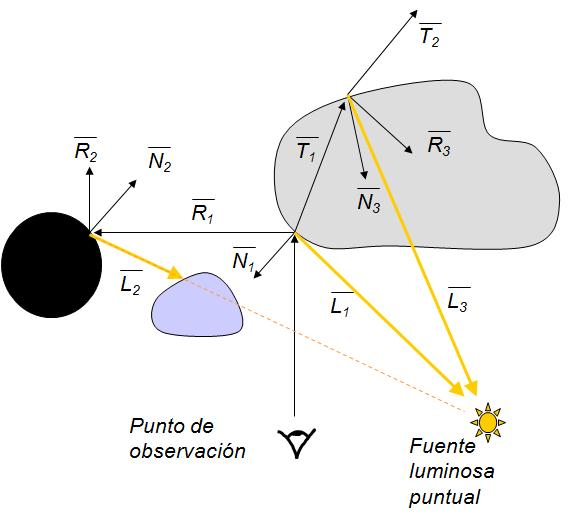
\includegraphics[width=0.7\textwidth]{../DOC_Relevamiento/exampleRT}
  \caption{Generaci�n de rayos del algoritmo de Whitted a partir de un �nico rayo primario.}
  \label{fig:exampleRT}
\end{figure}

En el primer nivel del algoritmo, cuando se traza un rayo primario, solo se tienen dos posibilidades: el rayo interseca con alg�n objeto de la escena o no lo hace. Si el rayo no encuentra ning�n objeto en su camino, entonces, se debe usar el color de fondo de la escena para pintar ese pixel. Por el contrario, si encuentra un objeto en su trayectoria, se deben realizar los siguientes pasos en el punto de intersecci�n:
\begin{itemize}
  \item Paso uno: para calcular las sombras, se traza un rayo de sombra ($L_{1}$) desde el punto de intersecci�n del rayo con el objeto hacia cada fuente de luz existente en la escena. Si alguno de estos rayos interseca cualquier objeto en su camino hacia la fuente de luz, dependiendo del material del objeto se debe calcular la cantidad de luz que pasa a trav�s de �l. Si el objeto es opaco, como es el caso del objeto m�s peque�o de la Figura~\ref{fig:exampleRT}, la luz es bloqueada totalmente y el punto de intersecci�n estar� bajo la sombra del objeto. Esto quiere decir que esta fuente de luz no ser� tomada en cuenta para calcular la iluminaci�n en el punto. Si el objeto es transparente, como es el caso del objeto m�s grande de la Figura~\ref{fig:exampleRT}, la intensidad de la fuente de luz se ve disminuida, incluso puede ser absorbida totalmente por el objeto. Existen tablas que indican que cantidad de luz es absorbida por cierto material transparente. En caso de que la luz no sea bloqueada totalmente por el objeto, esta contribuir� a la iluminaci�n del punto de intersecci�n del rayo primario.
  \item Paso dos: si el objeto tiene reflexi�n especular, como es el caso de la Figura~\ref{fig:exampleRT}, un rayo de reflexi�n es reflejado a partir del rayo primario, con respecto a la normal ($N_{1}$) en el punto de intersecci�n, en la direcci�n del vector $R_{1}$. Este rayo permite obtener la cantidad de luz que llega al punto de intersecci�n del rayo primario por el fen�meno de reflexi�n. Esta cantidad de luz puede verse afectada por el material del objeto, para considerar esto se usa un coeficiente dependiente del material, que escala la cantidad de luz.
  \item Paso tres: si el objeto es transparente, como es el caso de la Figura~\ref{fig:exampleRT} y no ocurre refracci�n total, es decir si la luz no es absorbida totalmente por la transparencia que posee el objeto, entonces un rayo de refracci�n es trazado a trav�s del objeto siguiendo la direcci�n del vector $T_{1}$. Esta direcci�n es calculada usando la ley de Snell \cite{LibroCompGrafica}. Este rayo permite obtener la cantidad de luz que llega al punto de intersecci�n del rayo primario por el fen�meno de refracci�n. Esta cantidad de luz puede verse afectada por el material del objeto, para considerar esto se usa un coeficiente dependiente del material, que escala la cantidad de luz.
\end{itemize}
Cada uno de los rayos de reflexi�n genera rayos de sombra, reflexi�n y refracci�n. Lo mismo sucede con cada uno de los de refracci�n. En el ejemplo de la Figura~\ref{fig:exampleRT}, para calcular la intensidad de luz aportada por $R_{1}$ se usan los mismos pasos que para calcular la intensidad aportada por el rayo primario. Por consiguiente los pasos dos y tres se deben calcular recursivamente. De esta manera se forma un �rbol de rayos para cada rayo primario, como se muestra en la Figura~\ref{fig:TreeExample}.
\begin{figure}[H]
  \centering
    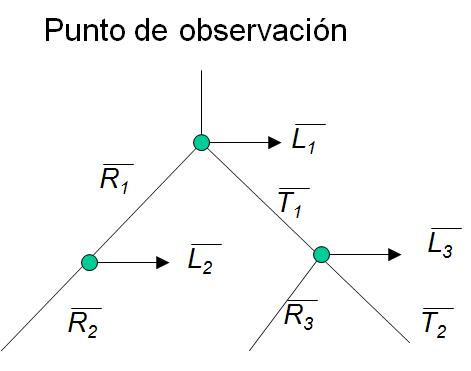
\includegraphics[width=0.7\textwidth]{../DOC_Relevamiento/TreeExample}
  \caption{�rbol de rayos que surge del ejemplo de la Figura~\ref{fig:exampleRT}.}
  \label{fig:TreeExample}
\end{figure}
La profundidad del �rbol de rayos afecta directamente el tiempo de ejecuci�n del algoritmo y la calidad de la imagen que se quiere obtener. Dicha profundidad est� determinada por distintos aspectos como por ejemplo un m�ximo dispuesto por el usuario del algoritmo o por no haber intersecci�n entre los rayos reflejados y refractados y alg�n objeto o por la capacidad de almacenamiento del sistema donde ejecuta el algoritmo.

Luego de obtener la cantidad de luz aportada por cada uno de los pasos anteriores, est�n dadas las condiciones para calcular la iluminaci�n en el punto de intersecci�n del rayo primario. Para esto se debe recorrer un �rbol de rayos (por ejemplo el de la Figura~\ref{fig:TreeExample}) de abajo hacia arriba, aplicando la ecuaci�n de iluminaci�n desarrollada por Whitted.

La ecuaci�n de Whitted que se presenta en la Ecuaci�n \ref{eqn:EcIluWhitted}, considera tres componentes, la primera es la iluminaci�n local, es decir, la iluminaci�n dada por el ambiente y por las fuentes de luz de la escena pero sin considerar que los objetos reflejan o refractan luz. Esta primera parte usa la ecuaci�n de iluminaci�n de Phong \cite{LibroCompGrafica}. La segunda ($k_{s}I_{r\lambda}$) y la tercera ($k_{t}I_{t\lambda}$) componente consideran la reflexi�n y la refracci�n de los objetos respectivamente.

\begin{equation}
    I_{\lambda} = I_{a\lambda}k_{a}O_{d\lambda}
                + \sum_{1 \leq i \leq m} S_{i} f_{att_{i}} I_{p\lambda_{i}} [k_{d}O_{d\lambda}(\overline{N} \cdot \overline{L_{i}})
                                                                            + k_{s} (\overline{N} \cdot \overline{H_{i}})^n]
                + k_{s}I_{r\lambda}
                + k_{t}I_{t\lambda}
    \label{eqn:EcIluWhitted}
\end{equation}

En la siguiente lista se puede observar el significado de cada variable presente en la Ecuaci�n \ref{eqn:EcIluWhitted}:
\begin{itemize}
  \item $I_{a\lambda}$ - Intensidad de la luz ambiente: luz que ha sido esparcida por todo el ambiente y es imposible determinar su origen, cuando golpea una superficie se esparce igualmente en todas direcciones.
  \item $k_{a}$ - Coeficiente de reflexi�n de luz ambiente: se encuentra entre 0 y 1. Determina la cantidad de luz ambiente reflejada por la superficie del objeto. Es una propiedad del material del objeto.
  \item $O_{d\lambda}$ - Componente difusa del color del objeto.
  \item $m$ - Cantidad de luces de la escena.
  \item $S_{i}$ - Indicador de sombra: indica si hay alg�n objeto entre la fuente de luz n�mero $i$ y el punto de evaluaci�n. Toma el valor 1 si la luz no est� bloqueada y 0 en caso contrario.
  \item $f_{att_{i}}$ - Factor de atenuaci�n para la luz n�mero $i$: soluciona el problema de que dos superficies se vean iguales al estar a distinta distancia de una fuente de luz. Lo m�s com�n es usar el inverso del cuadrado de la distancia hacia la luz.
  \item $I_{p\lambda_{i}}$ - Intensidad de la fuente de luz n�mero $i$ en el punto de evaluaci�n.
  \item $k_{d}$ - Coeficiente de reflexi�n de luz difusa: se encuentra entre 0 y 1. Determina la cantidad de luz difusa reflejada por la superficie del objeto. Es una propiedad del material del objeto.
  \item $k_{s}$ - Coeficiente de reflexi�n de luz especular: se encuentra entre 0 y 1. Determina la cantidad de luz especular reflejada por la superficie del objeto. Es una propiedad del material del objeto.
  \item $\overline{H_{i}}$ - Vector de direcci�n media o vector de iluminaci�n m�xima: vector utilizado por la ecuaci�n de iluminaci�n de Phong \cite{LibroCompGrafica}. Se calcula como la direcci�n media entre el vector normal y el vector que indica la direcci�n del observador.
  \item $n$ - Exponente de ajuste de la iluminaci�n: este exponente sirve para ajustar la imagen, no es un resultado te�rico sino que es resultado de la observaci�n emp�rica.
  \item $I_{r\lambda}$ - Intensidad del rayo reflejado: esta intensidad es determinada evaluando recursivamente la Ecuaci�n \ref{eqn:EcIluWhitted}.
  \item $k_{t}$ - Coeficiente de trasmisi�n: se encuentra entre 0 y 1. Determina la cantidad de luz que pasa a trav�s del objeto. Es una propiedad del material del objeto. Existen tablas con valores para distintos materiales.
  \item $I_{t\lambda}$ - Intensidad del rayo refractado: esta intensidad es determinada evaluando recursivamente la Ecuaci�n \ref{eqn:EcIluWhitted}.
\end{itemize}

\subsubsection{Algoritmo}

El algoritmo de Raytracing tiene como ventajas la simplicidad de su implementaci�n, as� como tambi�n el realismo que logra. Las simplificaciones que utiliza el modelo de iluminaci�n no permiten que se generen envolventes de los rayos de luz reflejados o refractados por una superficie curva. A los efectos generados por este fen�meno se les llama c�usticas. 

Otra simplificaci�n en el c�lculo de la iluminaci�n es la introducci�n de un componente de color de ``luz ambiente'', luz que tiene origen en alguna fuente de luz desconocida y parece llegar de todas las direcciones, esto permite no calcular algunos rebotes de la luz en objetos de la escena que har�an m�s complejo al algoritmo. Dada esta �ltima simplificaci�n tampoco se generan efectos de ``sangrado de luz'', este fen�meno es causado por la reflexi�n de luz de los objetos en forma parcial que hace que el color de una pared, por ejemplo, sea extendido por la zona del suelo cercana a la pared, dando la idea de que la pared ``sangra'' color sobre el suelo.

Una de las principales desventajas que muestra el algoritmo es el costo computacional en especial en los modelos utilizados en la mayor�a de las aplicaciones 3D basados en la ras\-te\-ri\-za\-ci\'on de im�genes formadas por pol�gonos. Por este motivo Raytracing no es una t�cnica utilizable para la aplicaciones que necesiten mostrar im�genes que se actualicen en tiempo real. Sin embargo, en los �ltimos tiempos se han desarrollado diferentes esfuerzos por alcanzar tiempo real en aplicaciones basadas en Raytracing, como por ejemplo el juego Quake 3 que utiliza el motor openRT, que utiliza un cluster de 20 nodos que cuentan con procesadores Athlon 64. Dependiendo de lo que se est� intentando dibujar en el juego en ese momento puede requerir algo m�s de capacidad de c�mputo para funcionar de manera adecuada.

En el Algoritmo \ref{alg:algoritmoRTracingI} se muestra un pseudoc�digo del algoritmo de Raytracing. 

\begin{algorithm}
    \caption{Pseudoc�digo del algoritmo de Raytracing.}
    \label{alg:algoritmoRTracingI}
    \begin{algorithmic}
        \ForAll{pixel $p$ en imagen a generar}
            \State $r = rayo(observador, p);$
            \State $p.color = trazarRayo(r, 1);$
        \EndFor
    \end{algorithmic}
\end{algorithm}

 En el Algoritmo \ref{alg:algoritmoRTracingII} se presenta el pseudoc�digo de la funci�n $trazarRayo$. Cada objeto de la escena es analizado para probar si el mismo es atravesado por el rayo; del conjunto de objetos atravesados interesa el objeto que tiene el punto de intersecci�n m�s cercano a la posici�n del observador. Una vez obtenido el punto de intersecci�n m�s cercano (si existe) se aplica la Ecuaci�n \ref{eqn:EcIluWhitted}.

La funci�n $verificarSombra$ del Algoritmo \ref{alg:algoritmoRTracingII} se resuelve lanzando un rayo desde el punto de intersecci�n hacia cada uno de los focos de luz para comprobar cuanta luz incide en el objeto. Si todos los rayos intersecan a un objeto antes de llegar al foco de luz entonces el punto est� en sombra, caso contrario se tendr� alguna funci�n que calcule cuanto aporta el foco a la iluminaci�n del punto.
Si el objeto atravesado m�s cercano tiene reflexi�n se genera un rayo reflejado con origen en la intersecci�n y cuya direcci�n es calculada en funci�n del �ngulo de incidencia del rayo original sobre la superficie del objeto. Si la superficie del objeto tiene refracci�n se genera un rayo refractado con origen en la intersecci�n cuya direcci�n es calculada en base a las densidades de los medios por los que atraviesa el rayo utilizando, por ejemplo, la ley de Snell \cite{LibroCompGrafica}. Los rayos reflejado y refractado se usan para invocar recursivamente. Con el color del objeto, el trazado de los rayos de sombra y las dos invocaciones recursivas, de reflexi�n y refracci�n se calcula el color del pixel invocando a la funci�n $calcularColorFinal$. Esta funci�n aplica la ecuaci�n de iluminaci�n del modelo de Whitted.


\begin{algorithm}
    \caption{Seudoc�digo de la funci�n trazarRayo.}
    \label{alg:algoritmoRTracingII}
    \begin{algorithmic}
        \Require Rayo $r$, Entero $profActual$
        \Ensure Color $color$
        \If {$profActual < MAXPROF$}
            \State \Return $colorNulo$;
        \EndIf

        \State $objetoMasCercano = \infty;$
        \ForAll{objeto $o$ en la escena}
            \If {$hayInterseccion(o, r)$}
                \If {$masCercaObservador(o, objetoMasCercano)$}
                    \State $objetoMasCercano = o;$
                \EndIf
            \EndIf
        \EndFor
        \If {$objetoMasCercano <> \infty$}
            \State $sombra = verificarSombra(objetoMasCercano,r,luces);$
            \If {$objetoMasCercano$ es reflectivo}
                \State $rR = rayoReflejado(objetoMasCercano, r);$
			    \State $reflex = trazarRayo(rR, profActual + 1);$
            \EndIf
            \If {$objetoMasCercano$ es transparente}
                \State $rT = rayoRefractado(objetoMasCercano, r);$
    			\State $refrac = trazarRayo(rT, profActual + 1);$
            \EndIf
            \State $color = calcularColorFinal(objetoMasCercano, sombra, reflex, refrac);$
        \Else
            \State $color = obtenerColorFondo(r)$;
        \EndIf
    \end{algorithmic}
\end{algorithm}


\subsubsection{Clasificaci�n de los algoritmos}

Todos los algoritmos, independientemente de la categor�a en la que se encuentren, buscan dada una escena, definici�n matem�tica o en alg�n tipo de representaci�n abstracta, generar una imagen en base a eso. En el trabajo se referencia siempre al concepto de  generaci�n de im�genes realistas aunque los mismos algoritmos podr�an ser utilizados para generar otro tipo de escenas. No obstante la diferencia de los enfoques de todos los algoritmos, todos buscan de alguna manera modelar la cantidad de energia lum�nica, o radiancia, que est� presente en cada punto los distintos objetos que forman la escena. De esta manera calcular de que manera se deber�a ver la imagen seg�n los par�metros de iluminaci�n que se establezcan. Las categor�as que se identifican son las siguientes.

\begin{itemize}
\item El modelo planteado por Whitted que fue descripto previamente.

\item El modelo basado en elementos finitos es bastante simple al igual que el modelo de Whitted pero a su vez muy diferente, ya que plantea para calcular la radiancia la divisi�n de la escena en peque�as partes y se utiliza alguna soluci�n num�rica para aproximar los valores.

\item Los algoritmos cuyo modelo de iluminaci�n est� basado en m�todos de Monte Carlo buscan aproximar los valores de radiancia en base a aproximaciones estad�sticas basadas en la integraci�n de Monte Carlo. Esta familia de algoritmos encuentra su mayor exponente actualmente en el algoritmo de Photon Mapping.
\end{itemize}

Por lo tanto Los algoritmos basados en Raytracing pueden ser clasificados utilizando distintas estrategias, en este trabajo se presentan agrupados por el modelo para el c�lculo de la iluminaci�n utilizado.

\begin{itemize}
  \item modelo simple de iluminaci�n local dise�ado por Whitted.
  \item modelo de iluminaci�n global.
      \begin{itemize}
        \item elementos finitos
        \item m�todos de Monte Carlo.
      \end{itemize}
\end{itemize}

\subsection{Radiosidad}
El algoritmo de radiosidad utiliza los principios de Raytracing para el c�lculo de las superficies visibles y sombras, as� como las reflexiones y refracciones pero a diferencia del algoritmo de Raytracing b�sico plantea que para hacer el c�lculo de la iluminaci�n es necesario pre calcular los valores de iluminaci�n en cada uno de los parches en los que se divide arbitrariamente la escena, por esta divisi�n es que este es un m�todo de elementos finitos. Luego de realizado el c�lculo de la radiancia de cada uno de los parches se utiliza un rastreo de la escena para el c�lculo de los valores de color de los pixels de la imagen que se quiere generar. Como se pre calculan los valores de la iluminaci�n en toda la escena a menos que se modifique la escena o las luces se pueden utilizar los mismos valores de radiancia pre calculados para generar im�genes desde distintos puntos de vista.
\subsection{Photon mapping}
Este algoritmo fue introducido por Henrik Wan Jensen en el a�o 1996\cite{Jensen2001}. Este algoritmo est� a�n en desarrollo dado que cuenta con una excelente calidad en las im�genes que puede generar y a su vez es computacionalmente menos costoso que el algoritmo de radiosidad. En lugar de utilizar el modelo de elementos finitos utiliza un modelo basado en m�todos de Monte Carlo para el c�lculo de la cantidad de energ�a en cada punto.
El algoritmo de Photon Mapping tiene dos etapas diferenciadas al igual que el algoritmo de radiosidad, pero tiene una aproximaci�n distinta para el c�lculo de la radiancia de los puntos. La primera pasada es similar a la recorrida de la escena por el algoritmo de Raytracing con la diferencia que sigue el sentido inverso. Esta primer pasada se llama emisi�n de fotones, se generan fotones, cuantos m�s se generen m�s fiable ser� el resultado de la iluminaci�n, que son lanzados desde los emisores de luz hacia la escena en direcciones que sean factibles. Se calcula el lugar en el que el fot�n incide en la escena recursivamente de manera an�loga al algoritmo de Raytracing. Esto es debido a que en el caso de los objetos reales, estos no absorben toda la luz incidente sino que hay luz que es reflejada y por lo tanto fotones son vueltos a lanzar desde el punto en el que chocaron con un objeto. Para hallar la direcci�n con la que es emitido el nuevo fot�n y la energ�a que tendr� el mismo se utiliza un modelo para los materiales de los objetos de la escena teniendo que agregar al material de los objetos una funci�n de BRDF (Funci�n de Distribuci�n de Reflectancia Bidireccional). Esta funci�n representa la proporci�n de radiaci�n reflejada por una determinada superficie en cada direcci�n del rayo reflejado, proyectada sobre el plano horizontal.


\section{Paralelizaci�n de algoritmos}

En noviembre de 2006 NVIDIA lanz� CUDA (Compute Unified Device Architecture), una arquitectura de computaci�n paralela de prop�sito general que hace uso del n�cleo de procesamiento paralelo de las GPU de NVIDIA para resolver una amplia variedad de problemas computacionales de una manera m�s eficiente que en una CPU. El modelo de programaci�n paralela propuesto por NVIDIA fue totalmente nuevo y la programaci�n sobre el mismo se hace a trav�s de un lenguaje de alto nivel, CUDA permite el uso del lenguaje C para la programaci�n.

Una ventaja muy importante del modelo es que cualquier aplicaci�n desarrollada en CUDA puede ejecutarse sobre cualquier n�mero de procesadores, sin necesidad de volver a compilar el c�digo. Esto permite crear aplicaciones capaces de escalar en el n�mero de procesadores, lo cual permite que una aplicaci�n ejecute en cualquier GPU que soporte CUDA.

El modelo de programaci�n esta basado en tres abstracciones fundamentales, dispone de una jerarqu�a de grupos de hilos de ejecuci�n, memoria compartida y barreras de sincronizaci�n de la ejecuci�n. Estas abstracciones gu�an al programador a dividir el problema en sub-problemas que pueden ser resueltos en forma paralela e independiente por medio de bloques de hilos de ejecuci�n. A su vez cada sub-problema de divide en piezas m�s chicas que pueden ser resueltas en paralelo y cooperando entre ellas, usando los hilos de ejecuci�n de cada bloque. Descomponer el problema de esta forma permite la escalabilidad autom�tica en el n�mero de procesadores, ya que cada bloque de hilos puede ser despachado hacia cualquier conjunto de procesadores (multiprocesador) disponible, en cualquier orden, concurrentemente o secuencialmente. De esta manera cualquier aplicaci�n CUDA puede ejecutar sobre cualquier n�mero de multiprocesadores y solo se necesita conocer este n�mero en tiempo de ejecuci�n. En la Figura \ref{fig:DiagramaEjecucionCUDA} se considera una aplicaci�n CUDA que esta dividida en cuatro bloques y se muestra como se asignan los bloques de hilos de ejecuci�n en dos GPU distintas, donde una tiene dos multiprocesadores y la otra tiene cuatro.

\begin{figure}[H]
    \centering
        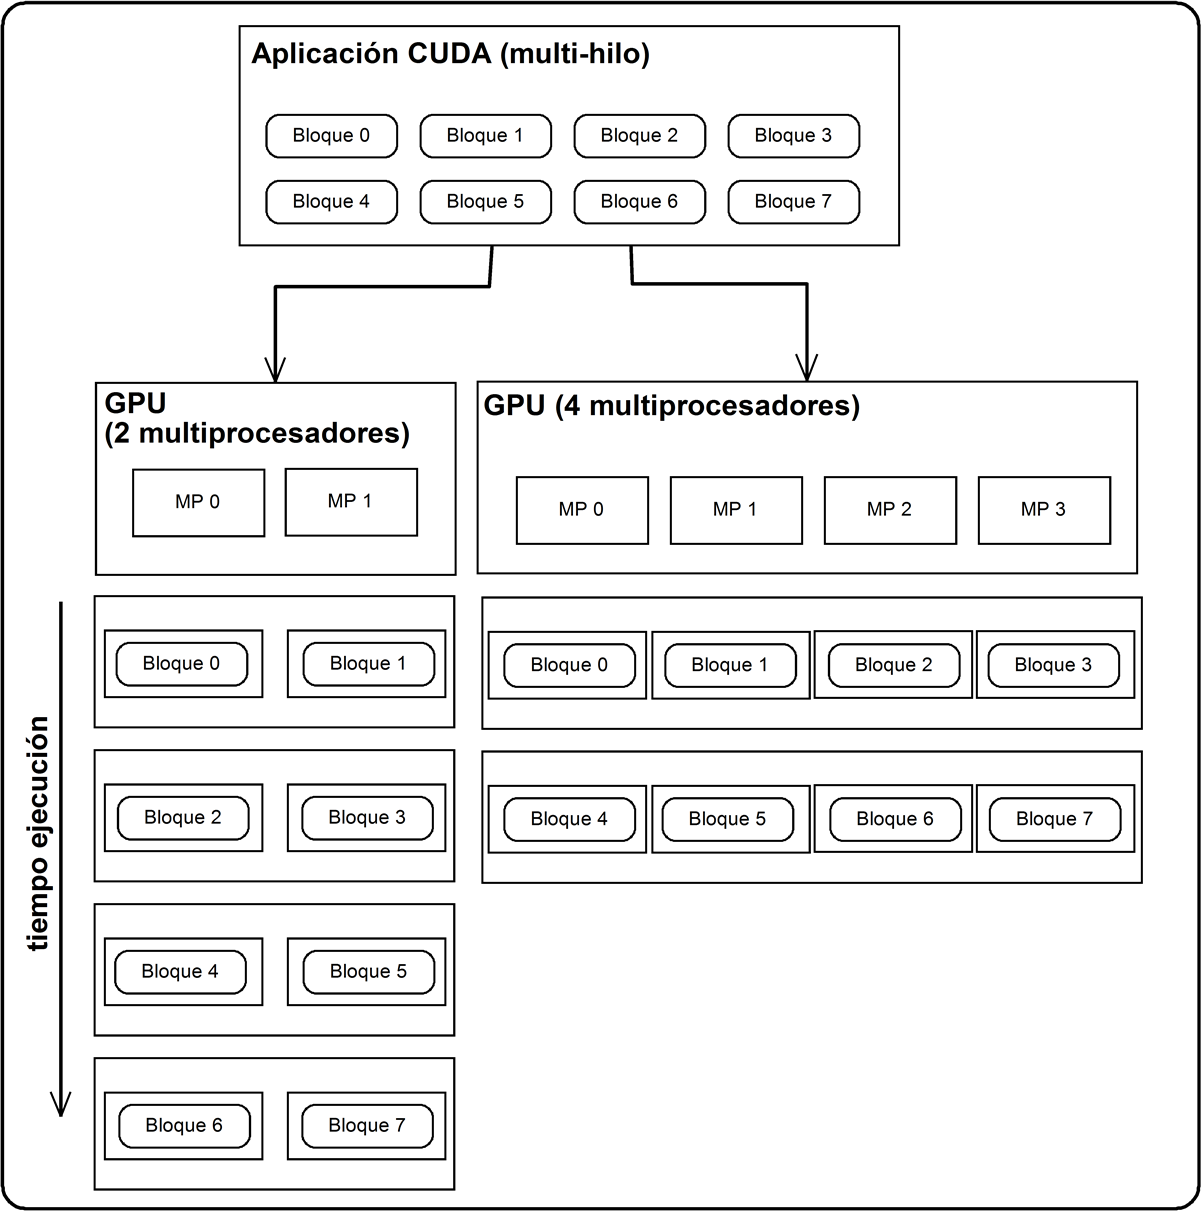
\includegraphics[width=0.8\textwidth]{./Capitulo4/diagramaEjecucionCUDA}
    \caption{Ejemplo de escalabilidad autom�tica en el n�mero de multiprocesadores.}
    \label{fig:DiagramaEjecucionCUDA}
\end{figure}


En la extensi�n del lenguaje C que hace CUDA es posible definir funciones (de la misma forma que en el lenguaje base) que a diferencia de las funciones normales de C, cuando son invocadas ejecutan $N$ veces en paralelo, mediante $N$ hilos de ejecuci�n de CUDA diferentes. Estas funciones propias de CUDA son llamadas \emph{kernels}. Dentro de este tipo especial de funciones se tiene acceso a informaci�n propia de CUDA que indica por ejemplo, el identificador del hilo de ejecuci�n o el identificador de bloque que lo contiene. Esta informaci�n es de vital importancia ya que es usada para parametrizar la ejecuci�n del \emph{kernel} en funci�n de los hilos de ejecuci�n.

Un \emph{kernel} siempre es invocado desde el \emph{host} (CPU) y ejecuta en el \emph{device} (GPU). La GPU act�a como co-procesador de la CPU y mediante \emph{kernels} la CPU puede asignar trabajo al co-procesador. En la Figura \ref{fig:ModeloKernels} se muestra un ejemplo de una aplicaci�n CUDA que posee un \emph{kernel} ``\emph{kernel A}''. Esta aplicaci�n comienza ejecutando c�digo secuencial en la CPU, en la primer parte secuencial se hace la invocaci�n al \emph{kernel}, el cual ejecuta en la GPU. Una vez terminada la ejecuci�n a nivel de GPU retorna a ejecutar c�digo secuencial en la CPU.

\begin{figure}[H]
    \centering
        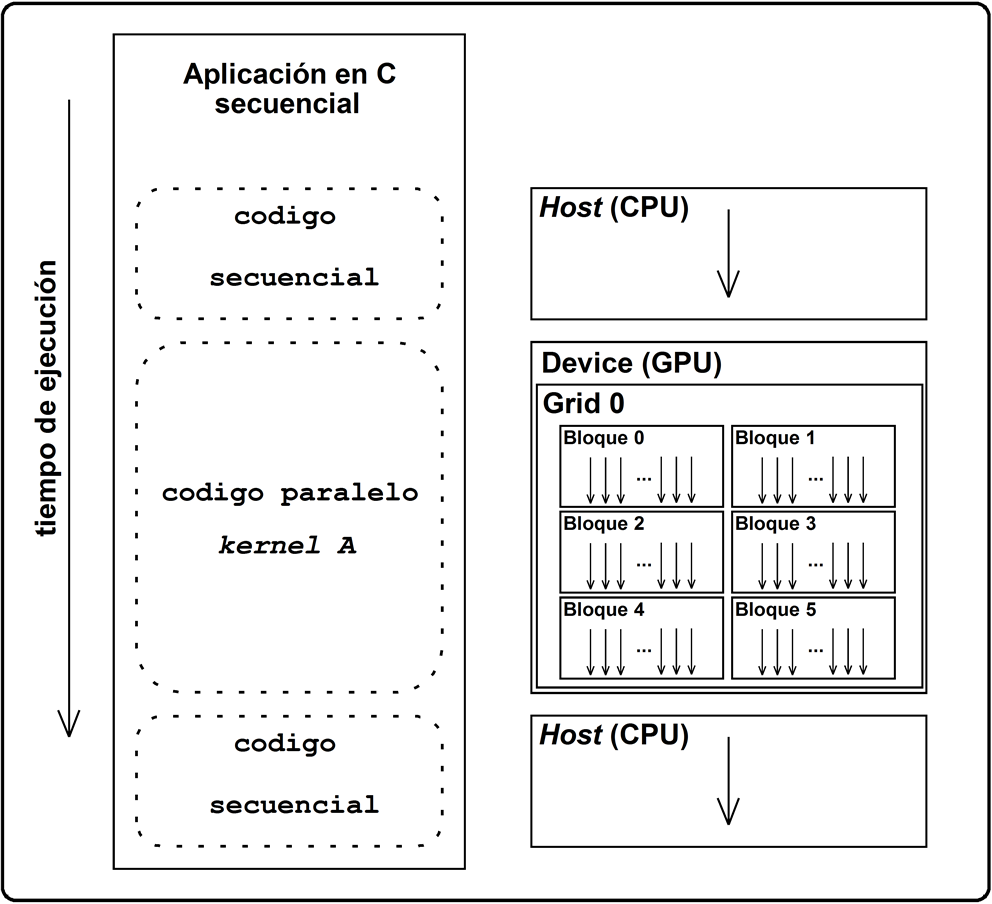
\includegraphics[width=0.8\textwidth]{./Capitulo4/modeloKernels}
    \caption{Ejemplo de ejecuci�n de una aplicaci�n CUDA.}
    \label{fig:ModeloKernels}
\end{figure}


El �ndice que identifica a un hilo de ejecuci�n es un vector tridimensional, usando el mismo un hilo puede ser identificado usando una, dos o tres componentes del vector. De esta manera los hilos pueden forman un bloque de una, dos o tres dimensiones. Esta forma de agrupar los distintos hilos de un bloque permite invocar \emph{kernels} sobre distintos tipos de dominio (vector, matriz o volumen) de una manera m�s natural. Los bloques tambi�n pueden ser agrupados una grilla (\emph{grid}) de una o dos dimensiones.

Cada hilo de CUDA puede acceder a m�ltiples espacios de memoria durante su ejecuci�n, mientras que los diferentes espacios de memoria forman la jerarqu�a de memoria de la GPU. Cada hilo de ejecuci�n tiene su propio espacio privado de memoria local. Cada bloque tiene un espacio de memoria compartida entre todos sus hilos, este espacio compartido tiene el mismo tiempo de vida que el bloque, es decir, es v�lido mientras el bloque se encuentra en ejecuci�n. Adem�s todos los hilos de ejecuci�n de la aplicaci�n tienen acceso a un mismo espacio de memoria global. Existen dos espacios m�s de solo lectura en la jerarqu�a que son accesibles por todos los hilos: el espacio de memoria constante y el espacio de memoria de textura. Ambos espacios de solo lectura tienen tiempo de vida igual al tiempo de ejecuci�n de la aplicaci�n CUDA y cada uno esta optimizado para distintos usos \cite{nVidiaCUDAWebSite}.



\chapter{Real Time} % 20 p�ginas mas o menos...

\section{Introducci�n}
Esta secci�n pretende entrar en detalle de los algoritmos y t�cnicas existentes para la aceleraci�n de la generaci�n de im�genes por computadora. Se ver�n los m�todos que fueron analizados y tenidos en cuenta a la hora de realizar este trabajo, centr�ndose en dos puntos principales que son: las estructuras de aceleraci�n espacial y la paralelizaci�n de procesos. Por un lado se busca reducir la cantidad de c�lculos requeridos para la generaci�n de una imagen y por otro lado hacer que los c�lculos se realicen en menos tiempo.

\section{Relevamiento}

\subsection{M�todos de aceleraci�n para raytracing}
El concepto de traza de rayos tiene muchas aplicaciones en computaci�n gr�fica, ejemplo de esto son los algoritmos de raycasting y raytracing de Whitted. Si bien estos algoritmos son diferentes entre si, tienen en com�n un aspecto: requieren trazar una enorme cantidad de rayos (generalmente millones) y gran parte de su tiempo de ejecuci�n es consumido por la traza de rayos.

A partir del reconocimiento del gran consumo computacional que significa trazar grandes cantidades de rayos, se torn� muy importante encontrar m�todos de a\-ce\-le\-ra\-ci�n para este proceso. Whitted al momento de desarrollar su algoritmo (en el a�o 1980) pudo apreciar que se gasta mucho tiempo en la traza de rayos. Desde ese momento hasta la actualidad se han propuesto diversas t�cnicas que buscan optimizar este proceso\cite{wald::PhD}.

Los m�todos de optimizaci�n propuestos hasta el momento pueden agruparse en dos categor�as principales, seg�n la forma de abordar el problema. A la primer categor�a pertenecen las t�cnicas que apuntan a reducir el n�mero de rayos a trazar. Hay dos caminos para lograr disminuir la cantidad de rayos, una forma es construir la imagen lanzando menos rayos primarios. Un ejemplo de este tipo de t�cnicas es la llamada \emph{adaptive sampling}. Usando este m�todo, para cada pixel de la imagen, se trazan rayos primarios por cada uno de sus v�rtices. Si la intensidad de la luz en cada una de las esquinas del pixel var�a significativamente con respecto a las otras, entonces el pixel es dividido en cuatro partes iguales. Luego se lanzan rayos primarios por cada nueva parte de la misma forma que se lanzaron en el pixel original. Las partes nuevas, si la intensidad de luz en sus esquinas difieren significativamente, se vuelven a dividir en cuatro y el proceso se repite. Esta subdivisi�n se repite hasta un nivel arbitrario, el cual debe establecerse buscando una buena relaci�n entre la calidad de la imagen y la aceleraci�n lograda. Cada parte comparte rayos con el nivel superior, lo que implica que no se deben lanzar cuatro rayos por parte en todos los casos. Una vez terminada la subdivisi�n el color del pixel es interpolado seg�n el color de cada una de sus partes\cite{wald::PhD}.

El otro camino es reducir el n�mero de rayos que deben ser trazados por cada rayo primario, es decir la cantidad de rayos secundarios. Un ejemplo de este tipo de t�cnicas es la llamada \emph{shadow caching}. La mayor�a de los rayos que se tranzan en un algoritmo de raytracing son rayos de sombra, ya que por cada rayo primario se trazan varios rayos de sombra. Para cada rayo de sombra se debe verificar si hay alg�n objeto en su camino hacia la fuente de luz y alcanza con que interseque con uno para garantizar oclusi�n. El cache de sombra explota el hecho de que muchos rayos se sombra son similares (sobre todo los que son originados por la misma fuente de luz) y que adem�s intersecan con el mismo objeto. En el cache se guarda para cada luz el �ltimo objeto que causo su oclusi�n. De esta manera, cada vez que se analiza un rayo de sombra se prueba primero si el mismo interseca con el objeto que se encuentra en el cache, para la fuente de luz que lo origino. Cuando hay varias fuentes de luz en la escena y hay un buen nivel de oclusi�n el cache de sombras reduce de manera importante el tiempo de procesamiento de los rayos de sombra\cite{wald::PhD}.

A la segunda categor�a pertenecen las t�cnicas que no se preocupan por reducir la cantidad de rayos lanzados para generar la imagen sino que buscan acelerar la intersecci�n de los rayos con la escena. Se puede lograr acelerar el n�cleo de los algoritmos de raytracing por varios caminos, eligiendo cuidadosamente las primitivas usadas para la construcci�n de las escenas y sus algoritmos de intersecci�n, usando vol�menes envolventes que permitan descartar primitivas que no sean alcanzadas por el rayo o utilizando divisiones espaciales (estructuras de aceleraci�n espacial) de la escena que garanticen no recorrer toda su lista de objetos por cada rayo que la atraviesa\cite{wald::PhD}.

\subsection{Estructuras de aceleraci�n espacial}
El algoritmo de trazado de rayos es una buena opci�n para generar im�genes de alta definici�n pero hay que considerar un inconveniente: es computacionalmente muy costoso. La principal raz�n de esto es la base del algoritmo, las intersecciones de los rayos con los objetos de la escena. Estas intersecciones son muy costosas de calcular porque para cada rayo y cada objeto de la escena hay que hacer un chequeo de intersecci�n. Si se consideran todos los chequeos necesarios para generar una imagen, estos pueden llegar a tomar el 95\% del tiempo de c�lculo \cite{TesisEstructuras}.
Se han desarrollado t�cnicas para optimizar el tiempo que toman las intersecciones rayo-objeto, basadas en tratar de minimizar el n�mero de intersecciones. A continuaci�n se muestran algunas (las m�s importantes seg�n Thrane y Ole \cite{TesisEstructuras}) de estas t�cnicas.

\subsubsection{Subdivisi�n espacial}
En el m�todo de subdivisi�n espacial el volumen de la escena se divide en regiones. A cada regi�n se le asigna una lista con todos los objetos que contiene, total o parcialmente. Estas listas se completan asignando a cada objeto la celda o las celdas que lo contienen. Esta t�cnica requiere un pre proceso para crear la estructura de datos donde quedar� registrada la informaci�n relativa al espacio que ocupan los objetos en la escena.

El pre proceso consiste en dividir el volumen total de la escena en peque�os vol�menes o voxeles (el t�rmino voxel es la extensi�n a tres dimensiones de su hom�nimo en dos dimensiones pixel). La forma de definir estos voxeles es lo que marca la diferencia entre las t�cnicas de subdivisi�n espacial. Una vez que los voxeles est�n definidos juegan el mismo papel en todas las t�cnicas.

La gran ventaja de esta t�cnica de subdivisi�n es que solo los objetos asignados a los voxeles atravesados por los rayos deben ser probados para una posible intersecci�n.

\paragraph{Subdivisi�n espacial uniforme.}
Cuando las particiones (voxeles) son todas del mismo tama�o la t�cnica se denomina subdivisi�n espacial uniforme. En la Figura \ref{fig:ExUniformGrid} se muestra un ejemplo de este tipo de subdivisi�n, que es totalmente independiente de la estructura de la escena.
\begin{figure}[H]
  \centering
    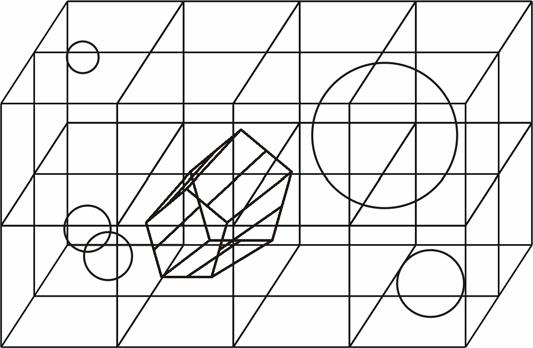
\includegraphics[width=0.7\textwidth]{../DOC_Relevamiento/exampleUniformGrid}
  \caption{Subdivisi�n espacial uniforme aplicada a una escena.}
  \label{fig:ExUniformGrid}
\end{figure}

Otro aspecto a tener en cuenta es que los voxeles se procesan en el mismo orden en que son encontrados por el rayo, lo que garantiza que cualquier voxel intersecado por un rayo estar� m�s cerca del origen del mismo que los restantes. Por consiguiente, una vez encontrado un punto de intersecci�n, por lo general no ser� necesario considerar el contenido de los restantes voxeles. Esto reduce considerablemente el n�mero de objetos que se han de probar para intersecci�n.
Cuando un rayo atraviesa un voxel, se tiene que averiguar si hay intersecci�n con cada uno de los objetos contenidos en �l, y se debe escoger la intersecci�n que se encuentre m�s cercana al origen del rayo.

\paragraph{Construcci�n.}
Dados los bordes de la escena y la lista de objetos de esta se puede construir la subdivisi�n espacial uniforme, el �nico par�metro necesario para su construcci�n es su resoluci�n a lo largo de los tres ejes imaginarios.

Seg�n Thrane y Ole no hay una t�cnica que garantice la mejor resoluci�n o por lo menos no para todos los casos. En el mismo trabajo se sugiere que la resoluci�n sea $3\sqrt[3]{N}$ voxeles a lo largo del eje m�s corto, donde $N$ es el n�mero de tri�ngulos de la escena. Aunque tambi�n se sugiere que puede ajustarse emp�ricamente para lograr �ptimos resultados en las im�genes.
Una vez que la resoluci�n es determinada, podemos construir una matriz tridimensional de listas de objetos que servir� para manejar los voxeles construidos y su contenido. Luego para cada objeto de la escena, se deben encontrar los voxeles que lo contienen y agregar una referencia al objeto a cada uno de ellos.

\paragraph{Acceso a los voxeles.}
La t�cnica usada para moverse a trav�s de los voxeles de la grilla es equivalente (para tres dimensiones) a la t�cnica para dibujar una l�nea en dos dimensiones. Este algoritmo es denominado Digital Differential Algorithm (DDA), fue propuesto por Fujimoto y es usado por Thrane y Ole, con algunas mejoras propuestas por Amanatides y Woo \cite{TesisEstructuras}.
En el Algoritmo \ref{alg:algoritmoDDA} se muestra un pseudoc�digo de la t�cnica para dos dimensiones para facilitar la comprensi�n (extenderla a tres dimensiones es simple).
\begin{algorithm}
    \caption{Recorrida de los voxeles atravesados por un rayo.}
    \label{alg:algoritmoDDA}
    \begin{algorithmic}
        \While{$X$ y $Y$ est�n dentro de la grilla}
            \State chequeo de intersecci�n con los tri�ngulos del voxel actual
            \If{hay intersecci�n en este voxel}
                \State se detiene el algoritmo y se retorna la intersecci�n
            \EndIf
            \If{$tmax_{x} < tmax_{y}$}
                \State $X \leftarrow X + step_{x}$
                \State $tmax_{x} \leftarrow tmax_{x} + delta_{x}$
            \Else
                \State $Y \leftarrow Y + step_{y}$
                \State $tmax_{y} \leftarrow tmax_{y} + delta_{y}$
            \EndIf
        \EndWhile\\
        \Return no hay intersecci�n
    \end{algorithmic}
\end{algorithm}

Antes de comenzar con el Algoritmo \ref{alg:algoritmoDDA} se debe identificar el voxel inicial, es decir el primer voxel que atraviesa el rayo. Si el origen del rayo se encuentra dentro de un voxel determinado, entonces este es el inicial. En caso contrario, se busca el primer punto de la grilla que interseca con el rayo y se usa este punto para localizar el voxel inicial. Las coordenadas de este se guardan en las variables $X$ e $Y$.
Adem�s se deben crear las variables $step_{x}$ y $step_{y}$, cuyos valores ser�n $\pm1$ dependiendo del signo de las componentes $x$ e $y$ del vector direcci�n del rayo. Estos valores ser�n usados para incrementar o decrementar las variables $X$ y $Y$, y as� ir avanzando a lo largo de la trayectoria del rayo.
Lo pr�ximo que se necesita es la m�xima distancia que se puede avanzar a lo largo de la trayectoria del rayo antes de cruzar un borde vertical o horizontal de un voxel. Estas distancias est�n representadas por las variables $tmax_{x}$ y $tmax_{y}$ respectivamente (ver Figura \ref{fig:ExampleDDA}). El m�nimo entre estas dos variables determina la m�xima distancia que se puede avanzar a trav�s de la trayectoria del rayo sin salir de los bordes del voxel actual.
Por �ltimo se calculan $delta_{x}$ y $delta_{y}$. La primera indica la distancia horizontal (en la trayectoria del rayo) que se debe avanzar para pasar al siguiente voxel. Esta se calcula de la siguiente manera: \[delta_{x} = \frac{voxelsize_{x}}{raydirection_{x}}\] La segunda variable indica la distancia vertical y se calcula de la misma forma.
Luego de la inicializaci�n de estas variables se usa un algoritmo (Algoritmo \ref{alg:algoritmoDDA}) incremental simple para avanzar a lo largo de los voxeles que el rayo atraviesa.
\begin{figure}[H]
  \centering
    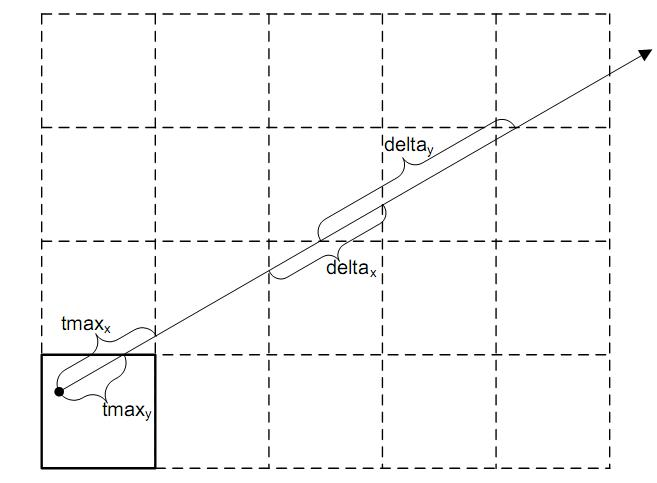
\includegraphics[width=0.7\textwidth]{../DOC_Relevamiento/algoritmoVoxels}
  \caption{Relaci�n entre el rayo, $tmax_{x}$, $tmax_{y}$, $delta_{x}$ y $delta_{y}$. El voxel inferior izquierdo contiene el punto origen del rayo.}
  \label{fig:ExampleDDA}
\end{figure}

\paragraph{Paralelismo en GPU.}
La subdivisi�n espacial uniforme fue implementada por primera vez sobre una GPU por Purcell y en ese momento se convirti� en la �nica estructura de aceleraci�n en ser paralelizada sobre GPU \cite{Purcell}.
En el trabajo de Thrane y Ole \cite{TesisEstructuras} se resumieron las principales razones por las cuales se considera a esta estructura buena para ser paralelizada sobre una GPU. Estas razones son:
\begin{itemize}
  \item Cada voxel atravesado por el rayo puede ser localizado y accedido en tiempo constante usando aritm�tica simple. Esto elimina la necesidad de recorrer �rboles (como en otras estructuras de aceleraci�n) y por lo tanto, el manejo de mucha informaci�n a nivel de la GPU, lo cual resulta muy costoso.
  \item El desplazamiento a trav�s de los voxeles atravesados se hace de forma incremental y con sumas sencillas, lo cual elimina la necesidad de una pila y hace posible visitar los voxeles en orden, es decir aumentando la distancia desde el origen del rayo.
  \item Se puede explotar el hecho de que los voxeles se recorren en orden para detener la recorrida cuando se de una intersecci�n en el voxel actual.
  \item El algoritmo de recorrido a trav�s de los voxeles que interseca el rayo esta dado por un vector lo cual es altamente compatible con el conjunto de instrucciones de una GPU.
\end{itemize}
En la subdivisi�n espacial se puede dar el caso de que un pol�gono sea referenciado por m�s de un voxel. Esto genera que en ocasiones especiales, se haga m�s de una vez el mismo test de intersecci�n. Para resolver esto se han generado t�cnicas como la denominada Mailboxing (esta t�cnica mantiene una tabla donde se asocia cada rayo con el �ltimo pol�gono al cual se le realiz� el test de intersecci�n). Al emplear estrategias de la paralelizaci�n este tipo de t�cnicas no pueden utilizarse, lo que implica que el algoritmo paralelo deber�a hacer chequeos repetidos \cite{TesisEstructuras}.

\subsubsection{KD-Trees}
\paragraph{Conceptos b�sicos.}
Al igual que la subdivisi�n espacial uniforme la estructura kd-tree es una instancia particular de la subdivisi�n espacial. La diferencia que tiene es que representa la escena con una estructura jer�rquica basada en un �rbol binario. En esta estructura se hace una distinci�n con respecto al tipo de los nodos, se distinguen los nodos internos de las hojas. Los nodos hoja se corresponden con los voxeles y tienen las referencias a los objetos que se encuentran dentro de los mismos. Los nodos internos se corresponden con la forma en que se divide el espacio. De esta manera, los nodos internos contienen un plano de corte y referencias a cada uno de los dos sub�rboles (cada hijo del nodo interno es un sub�rbol), mientras que los nodos hojas contienen listas de objetos.

Esta t�cnica de divisi�n del espacio tiene pr�cticamente las mismas ventajas que la subdivisi�n espacial uniforme con respecto a mejorar las intersecciones rayo-objeto. Ambas persiguen el mismo objetivo, que es minimizar la cantidad de intersecciones. Pero esta divisi�n intenta mejorar a la uniforme considerando que los objetos no est�n uniformemente distribuidos en la escena. La Figura \ref{fig:3D-Tree} muestra un ejemplo de divisi�n espacial usando un kd-tree. La primera divisi�n (rojo) corta la celda ra�z (blanco) en dos. Luego, se aplica otra divisi�n (verde) a estas celdas. La �ltima divisi�n (azul) se aplica a las 4 celdas existentes.

\begin{figure}[H]
  \centering
    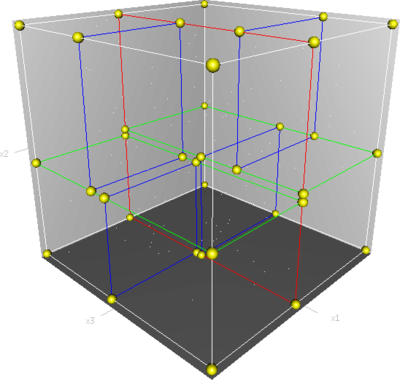
\includegraphics[width=0.7\textwidth]{../DOC_Relevamiento/3dtree}
  \caption{Subdivisi�n espacial usando una estructura kd-tree tridimensional.}
  \label{fig:3D-Tree}
\end{figure}

\paragraph{Construcci�n.}
La construcci�n de un kd-tree se hace de forma recursiva, siguiendo un enfoque top-down. Dada una caja que contenga completamente a la escena y una lista de objetos contenidos en ella, se escoge un plano de corte perpendicular a uno de los ejes de coordenadas, que divida la caja en dos. Al dividir se generan dos nuevos vol�menes, y cada uno de ellos es representado agregando un hijo al nodo asociado a la caja original. Cada uno de los objetos que contiene la caja original es asignado al nodo hijo que lo contiene. En caso de que un objeto tenga intersecci�n no vac�a con el plano de corte, entonces este objeto es asignado a ambos hijos.

Este procedimiento continua hasta que se alcanza una profundidad definida de antemano o hasta que el n�mero de objetos contenidos en cada voxel sea menor a un n�mero definido anteriormente. Havran \cite{Havran} sugiere que la profundidad m�xima sea igual a $16$ y que la cantidad de objetos por voxel sea $2$ para lograr un rendimiento �ptimo. Thrane y Ole \cite{TesisEstructuras} analizaron estos valores y concluyeron que $16$ como profundidad m�xima no era un buen valor para las escenas realistas. Se concluyo que, como la escena es dividida en dos en cada nivel del �rbol entonces, una profundidad m�s convincente ser�a una que fuera resultado de una funci�n logar�tmica en el n�mero de tri�ngulos de la escena. Esta consideraci�n tambi�n fue adoptada por Pharr y Humphreys \cite{PharrHumphreys}, los cuales usaron $8 + 1.3\log(N)$ como profundidad m�xima, donde $N$ es el n�mero de tri�ngulos de la escena.

La dificultad de construir esta estructura dado un volumen a dividir radica en escoger el lugar donde colocar el plano de corte. Thrane y Ole \cite{TesisEstructuras} usan una funci�n de costo para evaluar en donde se coloca el plano. Esta se basa en que la probabilidad de que un rayo atraviese un nodo hijo es proporcional a la proporci�n entre el �rea de la superficie del nodo hijo y el �rea de la superficie del nodo padre. Luego de algunos refinamientos la funci�n pasa a tener en cuenta tambi�n, lo que sucede cuando un objeto es cortado por el plano de corte. Esto es importante porque los objetos cortados se propagan a trav�s de los dos vol�menes hijos y por lo tanto se incurre en un alto costo de procesamiento. La forma de escoger una posici�n para el plano de corte es evaluar la funci�n de costo a lo largo de todos los ejes de las cajas que envuelven a los objetos de la escena. La posici�n con menos costo seg�n la funci�n es elegida para posicionar el plano. A modo de ejemplo se puede considerar la Figura \ref{fig:exFCKd-tree} donde se muestra el procedimiento para un solo eje, en el procedimiento real se deben considerar tambi�n los dos restantes \cite{TesisEstructuras}.

En la Figura \ref{fig:exFCKd-tree} la funci�n de costo es evaluada en los puntos $a, b, \ldots, j$. Estos puntos se corresponden con los puntos iniciales y finales de los intervalos que definen las cajas que envuelven a los objetos de la escena y el eje que ser� cortado. Vale la pena resaltar el intervalo $[c,f]$, que es generado por un objeto cortado por un plano, y es formado a trav�s de un recorte generado por el voxel actual.

\begin{figure}[H]
  \centering
    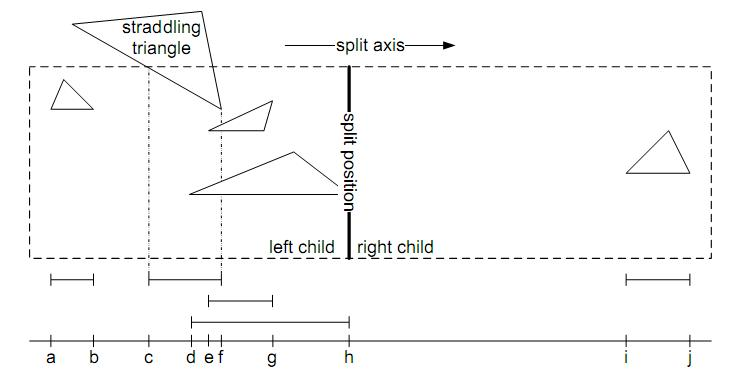
\includegraphics[width=0.7\textwidth]{../DOC_Relevamiento/exFCKd-tree}
  \caption{Ejemplo de b�squeda del plano de corte considerando solo un eje.}
  \label{fig:exFCKd-tree}
\end{figure}

En el caso que un objeto no est� completamente contenido en el voxel que se esta analizando para dividir, como sucede en el ejemplo de la Figura \ref{fig:exFCKd-tree}, no se debe usar la caja que lo envuelve totalmente. En este caso se debe cortar el objeto y usar solo la parte de este que queda contenida en el voxel que queremos dividir. De esta forma solo se considera la caja que envuelve totalmente a esta nueva parte. Esta t�cnica es denominada ``\emph{split clipping}'' \cite{Havran}. Aunque se considere el corte con respecto al voxel para obtener un nuevo volumen envolvente, el objeto que es transferido hacia los hijos del nodo actual es el objeto original y no el corte. Thrane y Ole \cite{TesisEstructuras} usan esta t�cnica para la construcci�n de la estructura kd-tree y obtuvieron muy buenos resultados.

En el Algoritmo \ref{alg:ConstruccionKD-Tree} se puede ver un seudoc�digo de la construcci�n de esta estructura. El algoritmo es recursivo, tiene como entrada un voxel y como salida una estructura kd-tree. En cada paso de la recursi�n se divide al voxel de entrada (nodo padre) en dos sub-voxels (nodos hijos). Para construir una estructura que permita lograr una buena aceleraci�n, el algoritmo busca el mejor plano de corte utilizando el m�todo que ilustra la Figura \ref{fig:exFCKd-tree}. Cada objeto perteneciente a la lista de objetos del nodo padre es agregado a la lista de objetos del nodo hijo que lo contiene total o parcialmente. Luego, para cada nodo hijo se invoca el algoritmo recursivamente.

El paso base de la recursi�n se da cuando se cumple alg�n criterio de parada. El algoritmo usa dos criterios de parada; cuando el n�mero de objetos del voxel de entrada es menor a cierto valor predefinido y cuando la profundidad de la recursi�n alcanza cierto valor predefinido.

Para construir una estructura kd-tree se invoca el algoritmo de cons\-truc\-ci�n con un voxel que contenga toda la escena. El algoritmo construye la estructura a partir de este voxel, dividi�ndolo hasta que se cumplan los criterios de parada para cada una de las ramas del �rbol de recursi�n.

\begin{algorithm}[H] %%% Algoritmo de la p�gina 46!
    \caption{Construcci�n de la estructura KD-Tree. Seudoc�digo de la funci�n $construir(voxel)$.}
    \label{alg:ConstruccionKD-Tree}
    \begin{algorithmic}
        \If {$numObjetos(voxel) \leq MIN\_OBJETOS$}
            \State se retorna nueva hoja con su lista de objetos
        \EndIf
        \If {$profundidad(arbol) \geq PROFUNDIDAD\_MAX$}
            \State se retorna nueva hoja con su lista de objetos
        \EndIf
        \State $mejorCorte \leftarrow \emptyset$
        \State $mejorCosto \leftarrow \infty$
        \ForAll {eje in \{$x, y, z$\}}
            \State $posiciones \leftarrow []$
            \ForAll {objeto en voxel}
                \State recortar objeto segun voxel
                \State calcular caja envolvente del objeto recortado
                \State encontrar puntos extremos a y b segun eje
                \State agregar a y b a la lista posiciones
            \EndFor
            \ForAll {punto p en posiciones}
                \If {$costo(p) < mejorCorte$}
                    \State $mejorCorte \leftarrow (p,eje)$
                    \State $mejorCosto \leftarrow costo(p)$
                \EndIf
            \EndFor
        \EndFor
        \State $(voxelIzq, voxelDer) \leftarrow dividir\ voxel\ segun\ mejorCorte$
        \ForAll {objeto o en voxel}
            \If {interseccion(o, voxelIzq)}
                \State agregar o a voxelIzq
            \EndIf
            \If {interseccion(o, voxelDer)}
                \State agregar o a voxelDer
            \EndIf
        \EndFor
        \State $hijoIzq \leftarrow construir(voxelIzq)$
        \State $hijoDer \leftarrow construir(voxelDer)$
        \State se retorna nuevoNodoInterno(hijoIzq, hijoDer, mejorCorte)
    \end{algorithmic}
\end{algorithm}

\paragraph{Acceso a los voxeles.}
Dado un nodo $N$ de un kd-tree, el algoritmo para moverse a lo largo del sub�rbol con ra�z $N$ debe seguir los siguientes pasos:
\begin{itemize}
  \item Si $N$ es un nodo hoja, todos los objetos de $N$ se prueban para ver si tienen intersecci�n con el rayo. En caso de que existan intersecciones, se retorna la m�s cercana al observador.
  \item Si $N$ es un nodo interno, es decir un nodo que esta dividido en dos y que tiene dos hijos, se debe determinar cual hijo de $N$ es atravesado primero por el rayo. Luego, se llama de forma recursiva con este nodo. Si esta llamada encuentra intersecci�n, ser� la m�s cercana al punto del observador entonces, se retorna. En caso contrario, se debe llamar de forma recursiva con el otro nodo hijo de $N$.
\end{itemize}
Utilizando el algoritmo para moverse en el �rbol, siempre se visitan los voxeles en el orden en que son visitados por el rayo. Esto permite que se pueda parar el algoritmo de recorrida de voxeles tan pronto como se encuentre la intersecci�n rayo-objeto m�s cercana al observador.

\paragraph{Paralelismo en GPU.}
El primer problema que surge al querer paralelizar el algoritmo de atravesado de voxeles en una GPU es que este es recursivo. Esto es un problema porque en la GPU no se cuenta con una pila.

Una soluci�n es considerar a la estructura kd-tree como un caso especial de la estructura de jerarqu�a de vol�menes envolventes (BVH, Bounding Volume Hierarchy) y usar su algoritmo de recorrida. Esto no es bueno porque se pierde la capacidad de recorrer los voxeles en el orden que son visitados por el rayo, y por lo tanto se pierde la capacidad de detener el algoritmo tan pronto como se encuentre una intersecci�n. Adem�s, como una estructura kd-tree es usualmente m�s grande que su correspondiente BVH para la misma escena, se estar�a creando un BVH ineficiente \cite{TesisEstructuras}. Una posible soluci�n es emplear una estrategia diferente de recorrido de los voxeles. Se puede emplear la estrategia usada por Foley y Sugerman \cite{FoleySugerman}, en la cual se cambia el algoritmo recursivo por uno secuencial. Esta estrategia consiste en mover un intervalo $[t_{min},t_{max}]$ a lo largo del rayo e ir descendiendo desde la ra�z del �rbol hasta que una hoja que contenga al intervalo sea encontrada. Inicialmente, el intervalo abarca todos los valores de $t$ tal que el punto $o + tv$ esta contenido en la caja del nivel superior del �rbol, es decir la caja que contiene a toda la escena ($o$ es el origen del rayo y $v$ es la direcci�n del rayo). Para cada nivel del �rbol que se desciende, se le asigna a $t_{max}$ el m�nimo entre $t_{max}$ y $t_{split}$, donde $t_{split}$ es la distancia a lo largo del rayo desde $t_{min}$ hasta el plano de corte del nodo actual. Cuando se llega a un nodo hoja, el intervalo es el rango param�trico en el cual el rayo se encuentra dentro del voxel determinado por el nodo.

Si en un nodo hoja se encuentra intersecci�n rayo-objeto, se debe retornar; por como lleva a cabo la recorrida el algoritmo, est� garantizado que esta ser� la intersecci�n m�s cercana al origen del rayo. En caso contrario, se debe actualizar el intervalo para continuar con la recorrida. El nuevo intervalo comienza en el fin del voxel actual y finaliza en el fin de la caja que contiene a la escena completa, como se muestra en el ejemplo de la Figura \ref{fig:TraversalKDTree}. En la parte (a) del ejemplo luego de que fallan todas las intersecciones en un nodo hoja, el nuevo intervalo es construido con el punto de fin del voxel actual y el punto de fin de la caja que envuelve a toda la escena. De esta manera, se llega a la siguiente hoja comenzando nuevamente el algoritmo de recorrida.
\begin{figure}[H]
  \centering
    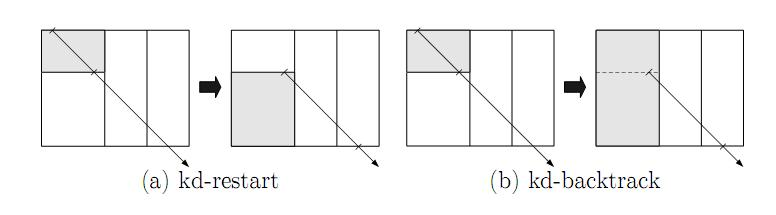
\includegraphics[width=0.8\textwidth]{../DOC_Relevamiento/traversal_kdtree}
  \caption{Actualizaci�n del intervalo en cada variante del algoritmo de atravesado.}
  \label{fig:TraversalKDTree}
\end{figure}

Foley y Sugerman presentan su algoritmo en dos variantes \emph{restart} y \emph{backtrack}. La variante \emph{restart} usa el enfoque de Glassner, en el cual se comienza desde la ra�z del �rbol cada vez que se avanza un voxel en la recorrida de los mismos \cite{Glassner84}. Esta t�cnica, en general, presenta un tiempo de  ejecuci�n alto y en este sentido es peor que el algoritmo recursivo.
Para remediar esto la t�cnica de \emph{backtrack} modifica la de \emph{restart} permitiendo moverse hacia arriba en el �rbol en vez de moverse hacia la ra�z cada vez. Cuando en un nodo hoja fallan todos los intentos por encontrar una intersecci�n, hay que moverse hacia arriba en la estructura de �rbol hasta que se encuentre un voxel ancestro que tenga intersecci�n con el nuevo intervalo. En la Figura \ref{fig:TraversalKDTree} parte (b) se muestra dicho ancestro marcado en color en la estructura de m�s a la derecha. Foley y Sugerman reportan una peque�a mejora utilizando esta t�cnica pero tambi�n afirman que se incurre en un grado m�s alto de complejidad en la implementaci�n.

En el trabajo de Horn et al. \cite{Horn07} se presentan optimizaciones que pueden realizarse sobre el algoritmo \emph{restart}. Los autores se�alan que en las pruebas realizadas, las optimizaciones propuestas permitieron llegar a un algoritmo de Raytracing con la capacidad de generar de 12 a 18 frames por segundo. Dado esto las consideran como buenas optimizaciones. Se llevaron a cabo tres optimizaciones sobre el algoritmo de Foley y Sugerman en su versi�n \emph{restart}:
\begin{itemize}
  \item Paquetes de rayos: esta optimizaci�n se basa en la idea de paquetes de rayos para CPUs, descrita por Wald \cite{Wald2001}. Wald busc� la manera de sacar provecho de las instrucciones SIMD de las CPUs modernas agrupando los rayos en paquetes. El tama�o de los paquetes queda determinado por la cantidad de datos que tengan como entrada las instrucciones. La mejora que introduce esta optimizaci�n es que todos los rayos de un mismo paquete se trazan en paralelo. Esta misma idea se puede llevar a una GPU, donde la cantidad de rayos por paquete depender� de las caracter�sticas de la misma.
  \item \emph{Push-Down}: esta optimizaci�n busca no recomenzar siempre desde la ra�z del �rbol. Por ejemplo, a menudo un rayo atraviesa el volumen que contiene a la escena y solo pasa a trav�s de un sub�rbol de la estructura kd-tree. Si se arranca el algoritmo siempre desde la ra�z se esta analizando muchas veces un sub�rbol que ya se sabe que no es atravesado por el rayo. Esta t�cnica permite recomenzar el algoritmo desde el sub�rbol m�s profundo que encierra al rayo, y de esta manera no se vuelven a analizar sub�rboles que no lo contienen.
  \item \emph{Short-Stack}: Horn et al. \cite{Horn07} observaron que era posible usar una pila que guarde los �ltimos N nodos visitados (tama�o fijo) y pasarse al algoritmo sin pila cuando esta se desborda. Dado esto, introdujeron como forma de optimizar el algoritmo una peque�a pila de tama�o fijo, cuya manipulaci�n puede tomar dos caminos. Cuando se introduce un nuevo nodo y la pila esta llena, se descarta el nodo que se encuentra m�s alejado del tope. Cuando se saca un nodo de la pila vac�a el algoritmo no termina, vuelve a comenzar desde la ra�z del �rbol. Esta pila es como un \emph{cach�} de nodos y puede ser usado para disminuir la frecuencia de recomienzos a costa de sacrificar el tiempo de procesamiento de un rayo.
\end{itemize}

\subsubsection{Jerarqu�a de Vol�menes Envolventes (BVH)}
\paragraph{Conceptos b�sicos.}
La estructura BVH divide la escena y guarda la informaci�n de la divisi�n en una jerarqu�a definida por un �rbol. Difiere de las t�cnicas de subdivisi�n espacial porque no divide el espacio sino que divide objetos. El volumen envolvente de una pieza de geometr�a es un objeto geom�trico simple que la envuelve, es decir que la contiene en su interior. Claramente, si falla la intersecci�n de un rayo con el volumen envolvente de un objeto, falla la intersecci�n con cualquier cosa que este dentro del mismo y por lo tanto falla la intersecci�n rayo-objeto.

La motivaci�n para usar vol�menes envolventes es que realizar un chequeo de intersecci�n con un objeto simple, como lo es un volumen envolvente, es mucho menos costoso que hacerlo contra el objeto que contiene dentro, que por lo general no es un objeto simple. La aceleraci�n que se logre mediante esta t�cnica depender� de la complejidad de los objetos de la escena y de los vol�menes envolventes que se usen.

Una jerarqu�a de vol�menes envolventes esta formada por un nodo ra�z que contiene un volumen que envuelve a todos los dem�s vol�menes, y tambi�n contiene a todos los objetos de la escena. Cada nodo interno del �rbol tiene como hijos a un conjunto de nodos internos, cada uno de ellos con un volumen envolvente asociado, o a un conjunto de nodos hoja, con un n�mero cualquiera de objetos de la escena asociados. En la Figura \ref{fig:BVHExample} se muestra una estructura BVH como ejemplo, la cual utiliza cajas alineadas a los ejes como vol�menes envolventes. Es posible utilizar otros objetos envolventes, por ejemplo, cajas no alineadas a los ejes, cilindros, esferas, etc.

El algoritmo de recorrida de los vol�menes envolventes es realizado usando un simple e intuitivo descenso recursivo.

\begin{figure}[H]
  \centering
    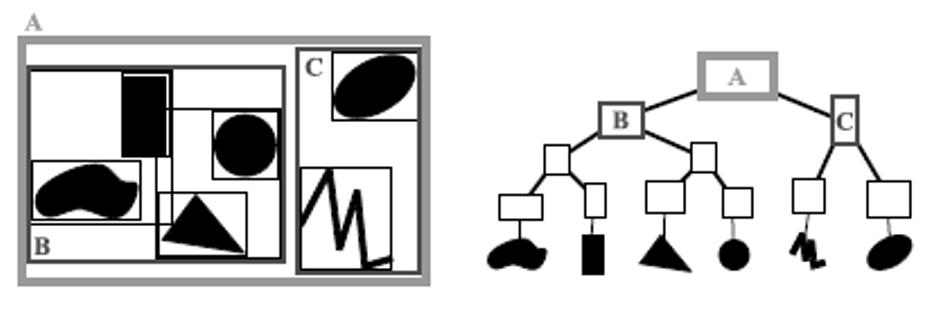
\includegraphics[width=0.9\textwidth]{../DOC_Relevamiento/BVHExample}
  \caption{Ejemplo de estructura BVH que utiliza cajas alineadas a los ejes.}
  \label{fig:BVHExample}
\end{figure}

\paragraph{Construcci�n.}
Una medida razonable de la calidad de una estructura BVH, es el costo promedio de aplicarle el algoritmo de recorrida, dado un rayo arbitrario. No hay ning�n algoritmo conocido que construya estructuras BVH �ptimas, tampoco es obvio como evaluar el costo promedio de atravesar con un rayo arbitrario una estructura de este tipo.
Goldsmith y Salmon proponen una funci�n de costo conocida como la heur�stica del �rea de las superficies \cite{GoldsmithSalmon}. Est� formalizada usando el �rea de la superficie del nodo padre y del nodo hijo y sigue la relaci�n de la Ecuaci�n \ref{eqn:AreasSuperficies}.
\begin{equation} %%% Ecuacion pagina 53!!!
    P(hit(c) | hit(p)) \approx \frac{S_{c}}{S_{p}}
    \label{eqn:AreasSuperficies}
\end{equation}

Donde:
\begin{itemize}
  \item $hit(n)$ es el evento en que el rayo atraviesa el nodo $n$.
  \item $S_{n}$ es el �rea de la superficie del nodo $n$.
  \item $c$ y $p$ son el nodo hijo y padre, respectivamente.
\end{itemize}
La funci�n da un estimativo del costo de la jerarqu�a cuando se trata de atravesar por un rayo cualquiera.

Como no existe un algoritmo para construir eficientemente una estructura BVH �ptima, se han propuesto heur�sticas de construcci�n. Por lo general, estas heur�sticas se basan en una de las dos ideas propuestas por Kay y Kajiya \cite{KayKajiya} y Goldsmith y Salmon \cite{GoldsmithSalmon}, las cuales se presentan a continuaci�n.

Antes de presentar las ideas para construir una estructura BVH es importante considerar que en la pr�ctica, los vol�menes m�s usados para construir una BVH son los vol�menes envolventes alineados a los ejes de coordenadas (AABB). Los AABB pierden rendimiento porque no se ajustan perfectamente a los objetos, pero lo ganan por el lado de permitir un chequeo de intersecci�n simple y r�pido. Tambi�n son muy buenas estructuras en t�rminos de simplicidad de implementaci�n \cite{TesisEstructuras}. Los dos enfoques de construcci�n que se presentan a continuaci�n utilizan este tipo de volumen envolvente.

Kay y Kajiya sugieren un enfoque recursivo top-down. Esta idea se muestra aplicada al algoritmo de construcci�n en el Algoritmo \ref{alg:ConstruccionBVH}. Para construir una estructura BVH el algoritmo necesita como entrada la lista de objetos que conforman la escena. La salida del algoritmo es una jerarqu�a de vol�menes envolventes alineados con los ejes, como la que se muestra en la Figura \ref{fig:BVHExample}. Si la escena tiene un solo objeto, la estructura se construye con un solo volumen envolvente. En caso contrario, se busca el mejor eje de corte y la mejor posici�n de corte. Se pueden usar diversas estrategias para encontrar el plano de corte, una de ellas es usar la funci�n de costo que se muestra en la Ecuaci�n \ref{eqn:AreasSuperficies}. Se puede adoptar otra estrategia como cortar siempre por el punto medio o como dejar la misma cantidad de objetos de cada lado del plano. Por �ltimo, se construyen los sub�rboles izquierdo y derecho de forma recursiva, as� como tambi�n se construye el volumen envolvente que contiene a todos los objetos.

\begin{algorithm} %%% Algoritmo de la p�gina 54!!!
    \caption{Construcci�n de la estructura BVH seg�n Kay y Kajiya \cite{KayKajiya}. Seudoc�digo de la funci�n $consArbol(objetos)$}
    \label{alg:ConstruccionBVH}
    \begin{algorithmic}
        \State BVNODE res
        \If {cantidad(objetos) == 1}
            \State $res.hijoIzq \leftarrow arbolVacio$
            \State $res.hijoDer \leftarrow arbolVacio$
            \State $res.volEnvolvente \leftarrow volumen\ que\ contiene\ a\ todo\ o \in objetos$
        \Else
            \State Calcular el mejor eje de corte y por donde se debe cortar
            \State $res.hijoIzq \leftarrow consArbol(objetos\ del\ lado\ izquierdo\ del\ corte)$
            \State $res.hijoDer \leftarrow consArbol(objetos\ del\ lado\ derecho\ del\ corte)$
            \State $res.volEnvolvente \leftarrow volumen\ que\ contiene\ a\ todo\ o \in objetos$
        \EndIf
        \State se retorna res
    \end{algorithmic}
\end{algorithm}

Goldsmith y Salmon proponen un enfoque de construcci�n bottom-up que resulta m�s complicado. El algoritmo comienza asignando el primer objeto de la escena como la ra�z del �rbol. Para cada objeto adicional en la escena, se busca la mejor posici�n en el �rbol mediante la evaluaci�n de una funci�n de costo (por ejemplo, usando la Ecuaci�n \ref{eqn:AreasSuperficies}). La posici�n se busca mediante un recorrido recursivo descendente en el �rbol, siguiendo el camino que resulte menos costoso seg�n la funci�n. Finalmente, el objeto es insertado de alguna manera: como una nueva hoja o se reemplaza una hoja existente por un nodo interno que contiene al nodo hoja viejo y al nuevo objeto como hijos. Como resultado de este enfoque un nodo interno puede tener un n�mero arbitrario de hijos, contrariamente a lo que pasa con el enfoque de Kay y Kajiya, que produce �rboles binarios.

Goldsmith y Salmon advierten que la calidad de la estructura BVH generada por su algoritmo depende fuertemente del orden de los objetos pasados como entrada. Como una soluci�n, recomiendan distribuir aleatoriamente el orden de los objetos antes de construir la estructura.

\paragraph{Acceso a los vol�menes envolventes.}
La forma est�ndar de recorrer una estructura BVH es a trav�s de una recursi�n. Para los nodos internos se debe probar la intersecci�n del rayo contra el volumen envolvente asociado. Si se encuentra intersecci�n, se debe probar la intersecci�n recursivamente contra los nodos hijos. A diferencia de la estructura kd-tree, se deben visitar todos los nodos hijos, dado que estos se pueden solapar y no siguen ning�n criterio de ordenaci�n. Si el rayo no atraviesa el volumen envolvente del nodo no es necesario probar los nodos hijos. Para los nodos hoja, solo se debe probar si el rayo tiene intersecci�n con alguno de los objetos de la escena asociados al nodo.

El principal problema que se encuentra cuando se quiere acceder a los vol�menes envolventes para probar su intersecci�n con el rayo, es el orden en el cual los nodos hijos son accedidos. Kay y Kajiya proponen un m�todo por el cual se intenta seleccionar el nodo m�s cercano al origen del rayo, siguiendo la direcci�n del mismo. Esta t�cnica es un poco complicada porque requiere por ejemplo, mantener una cola de prioridad, de donde se extraen los nodos a ser atravesados por el rayo. Thrane y Ole \cite{TesisEstructuras} concluyen que esta t�cnica no implica una ganancia de rendimiento considerable.

\paragraph{Paralelismo en GPU.}
Para implementar en una GPU el algoritmo que atraviesa una estructura BVH dado un rayo hay que resolver dos problemas. El primero corresponde a encontrar un m�todo para atravesar la estructura de �rbol eficientemente sin contar con una pila. El segundo problema es encontrar una representaci�n adecuada de la estructura BVH para usar sobre la GPU.

La representaci�n de la estructura y el algoritmo que atraviesa el �rbol son independientes. La soluci�n propuesta por Thrane y Ole se basa en una cuidadosa elecci�n de los datos que se deben guardar dados los tipos de almacenamiento que provee la GPU. En la GPU se debe guardar el estado del recorrido en vez de guardar el �rbol en si mismo. La idea para llevar a cabo esto proviene de observar que los rayos atraviesan los nodos del �rbol siempre en \emph{pre-order}. Una recorrida de un �rbol es en \emph{pre-order} cuando se recorre primero el nodo ra�z, luego el sub�rbol izquierdo y por �ltimo el sub�rbol derecho, como se muestra en el ejemplo de la Figura \ref{fig:TraversalBVH}.

\begin{figure}
  \centering
    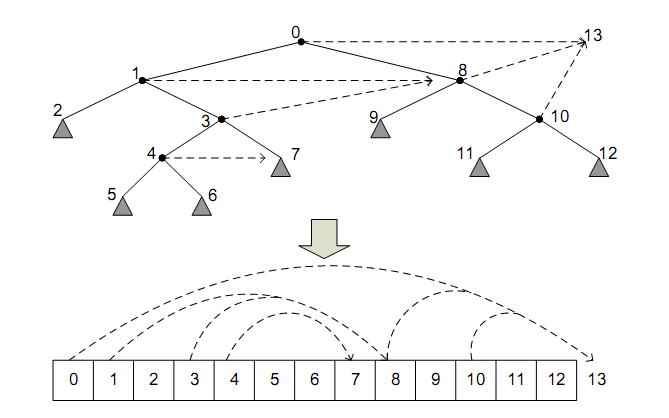
\includegraphics[width=0.8\textwidth]{../DOC_Relevamiento/traversalBVH}
  \caption{Ejemplo de codificaci�n de los datos para atravesar una estructura BVH.}
  \label{fig:TraversalBVH}
\end{figure}

Los nodos del �rbol son numerados secuencialmente de acuerdo al orden mencionado anteriormente. Esta numeraci�n coincide con la forma en que son guardados los datos de los nodos en la estructura que maneja la GPU, un array.

Una l�nea punteada $(a \dashrightarrow b)$ representa la situaci�n en la que el rayo no atraviesa al volumen $a$ y se debe seguir probando con los dem�s nodos hermanos, en este caso el volumen $b$. Como se muestra en la Figura \ref{fig:TraversalBVH}, cada l�nea punteada es guardada como un par de �ndices, donde cada componente del par hace referencia al array. Thrane y Ole \cite{TesisEstructuras} llaman a este puntero �ndice de escape. En el ejemplo de la Figura \ref{fig:TraversalBVH}, si un rayo no atraviesa el volumen n�mero 1 se debe seguir probando con los vol�menes hermanos del mismo para ver si el rayo atraviesa a alguno de ellos. Para pasar del volumen n�mero 1 a su proximo hermano (volumen n�mero 8) sin tener que recorrer todo el sub�rbol izquierdo se usa el �ndice de escape $(1 \dashrightarrow 8)$. A trav�s del �ndice de escape se navega el �rbol de forma eficiente. Se puede ver claramente que todos los nodos hoja tienen un �ndice de escape relativo igual a $1$. Como consecuencia de esto, no se necesita guardar a la vez el �ndice de escape y los objetos que contiene el volumen. Notar la convenci�n indirecta en la Figura \ref{fig:TraversalBVH} donde los nodos internos del sub�rbol derecho tienen �ndice de escape igual al n�mero total de nodos del �rbol. Esto se usa para tener un criterio de parada en el algoritmo de recorrida.

Un algoritmo para atravesar una estructura BVH dado un rayo que siga este enfoque es simple e iterativo, lo cual es muy bueno para ejecutarlo en una GPU. El algoritmo requerido para ejecutar la recorrida de los vol�menes envolventes de una BVH, guardados en la estructura de array, es mostrado en el Algoritmo \ref{alg:TraversalBVH}. La iteraci�n siempre termina con un �ndice actual mayor al que exist�a cuando se inici�, esto se da como consecuencia de que los �ndices de escape siempre van en la direcci�n de aumento.

\begin{algorithm} %%% Algoritmo de la p�gina 57!!!
    \caption{recorrida de los volumenes envolventes para GPU.}
    \label{alg:TraversalBVH}
    \begin{algorithmic}
        \State $S \leftarrow secuencia\ de\ recorrida$
        \State $r \leftarrow el\ rayo$
        \State $indiceActual \leftarrow 0$
        \While {$indiceActual < largo(S)$}
            \State $nodoActual \leftarrow S[indiceActual]$
            \If {$hayInterseccion(r, nodoActual)$}
                \State $indiceActual \leftarrow indiceActual + 1$
                \State guardar datos interseccion si $nodoActual$ es hoja
            \Else
                \State $indiceActual \leftarrow indiceEscape(nodoActual)$
            \EndIf
        \EndWhile
    \end{algorithmic}
\end{algorithm}


\subsubsection{Conclusiones}

\begin{table}[!hbt]
\begin{center}
\resizebox{12cm}{!}{
    \begin{tabular}{|p{4cm}|c|c|c|}
    \hline
    &SEU & Kd-Tree & BVH\\
    \hline
    Complejidad del algoritmo de construcci�n & \multirow{2}{*}{Media} & \multirow{2}{*}{Alta} & \multirow{2}{*}{Baja}\\
    \hline
    Aceleraci�n lograda & Baja & Media & Alta\\
    \hline
    Adaptaci�n frente a escenas no uniformes & \multirow{2}{*}{Baja} & \multirow{2}{*}{Media} & \multirow{2}{*}{Alta}\\
    \hline
    Consumo de memoria & Medio & Alto & Bajo\\
    \hline
    Complejidad del algoritmo de atravesado & \multirow{2}{*}{Media} & \multirow{2}{*}{Alta} & \multirow{2}{*}{Baja}\\
    \hline
    Adaptaci�n frente a escenas est�ticas & \multirow{2}{*}{Mala} & \multirow{2}{*}{Buena} & \multirow{2}{*}{Mala}\\
    \hline
    Adaptaci�n frente a escenas din�micas & \multirow{2}{*}{Mala} & \multirow{2}{*}{Mala} & \multirow{2}{*}{Buena}\\
    \hline
    \end{tabular}
}
\caption{Comparaci�n de las estructuras de aceleraci�n}
\label{table:ConclusionesEstructuras}
\end{center}
\end{table}

Thrane y Ole \cite{TesisEstructuras} analizan experiencias obtenidas al implementar y usar la subdivisi�n espacial uniforme en la paralelizaci�n del algoritmo de trazado de rayos. La aceleraci�n lograda a trav�s de esta estructura es menor que la obtenida a trav�s de Kd-Tree o BVH, excepto para algunas escenas con objetos simples. Esto permite concluir que la estructura no es buena para escenas donde se dan grandes variaciones en la densidad de los objetos, desde el punto de vista geom�trico. Tambi�n se destaca que el algoritmo para recorrer los voxeles atravesados requiere guardar mayor cantidad de datos para representar el estado del recorrido, en comparaci�n con las estructuras Kd-Tree y BVH. Los autores concluyen que el algoritmo de recorrida de los voxeles se puede paralelizar en una GPU pero que tiene un bajo rendimiento, en comparaci�n con el obtenido al usar las estructuras Kd-Tree o BVH. Seg�n Thrane y Ole \cite{TesisEstructuras}, para algunos casos de prueba de su trabajo donde la resoluci�n de la grilla es grande el algoritmo de recorrida de los voxeles tiene un tiempo de ejecuci�n mayor al tiempo de la estructura Kd-Tree o al de la BVH.

Por otro lado, Thrane y Ole \cite{TesisEstructuras} implementaron la estructura de aceleraci�n Kd-Tree sobre GPU. Usaron ambas t�cnicas (\emph{restart} y \emph{backtrack}) y concluyeron que para la mayor�a de las escenas, esta estructura mejora en rendimiento a la subdivisi�n espacial uniforme. Tambi�n se recalca que las dos t�cnicas para realizar la recorrida a trav�s de los voxeles sufren de alta complejidad en sus algoritmos (en el contexto de una GPU) y esto no es deseable ya que aumenta el tiempo de ejecuci�n. Aunque tambi�n se menciona que el tiempo de ejecuci�n que se agrega por la complejidad puede verse compensado, en cierto grado, por la habilidad de la estructura para adaptarse a los cambios de densidad de objetos en la escena.

En el trabajo de Lauterbach et al. \cite{Lauterbach06} luego de haber usado la estructura Kd-Tree para diversos casos de prueba se lleg� a la conclusi�n de que con esta se obtienen mejores resultados de los que se obtienen utilizando la estructura BVH, para escenas est�ticas (las escenas est�ticas se caracterizan por componerse de objetos fijos, que no cambian de posici�n ni de forma en el tiempo). Esta ganancia en rendimiento tiene como costo asociado un mayor consumo de memoria y una mayor complejidad para implementar y optimizar la construcci�n de la estructura.

Con respecto a la estructura BVH, Thrane y Ole \cite{TesisEstructuras} implementaron sobre una GPU ambas estrategias de construcci�n, el enfoque top-down y el bottom-up, para comparar resultados. Usaron siempre vol�menes envolventes alineados a los ejes, en ambas construcciones. La estrategia de recorrida a lo largo de los nodos hijos fue siempre de izquierda a derecha. Esto en algunos casos no result� muy eficiente ya que si el rayo atraviesa todos los vol�menes envolventes y el volumen donde se da la intersecci�n m�s cercana es el �ltimo de una lista de hermanos, se debe revisar todos los dem�s vol�menes antes de llegar a un resultado. En un caso de este tipo pr�cticamente se est� utilizando fuerza bruta para encontrar la intersecci�n, cosa que se buscaba evitar con la introducci�n de estructuras de aceleraci�n. Una alternativa es recorrer la lista de hermanos seg�n la direcci�n del rayo pero los autores optaron por no mejorar este aspecto para mantener la simplicidad en el algoritmo (ya que debe ser implementado en una GPU).

La gran ventaja de la estructura BVH es la simplicidad del algoritmo de recorrida y la gran desventaja es el orden fijo en que se recorren los nodos hermanos \cite{TesisEstructuras}. Adem�s Thrane y Ole \cite{TesisEstructuras} concluyeron que esta estructura es la que tiene mejor rendimiento sobre la GPU, comparando con la subdivisi�n espacial uniforme y con la BVH. Como un agregado se destaca que la implementaci�n de la construcci�n y de la recorrida de los vol�menes es m�s simple que cualquier otra estructura que se quiera implementar sobre una GPU.

Lauterbach et al. \cite{Lauterbach06} luego de haber usado la estructura BVH para diversos casos de prueba concluy� que con esta estructura se obtienen mejores resultados de los que se obtienen utilizando la Kd-tree, para escenas din�micas (las escenas din�micas se caracterizan por componerse de objetos que a medida que el tiempo avanza cambian de posici�n, forma, etc.). Adem�s, los autores se�alan que a la jerarqu�a de vol�menes envolventes es m�s f�cil agregarle la optimizaci�n basada en paquetes de rayos que a la Kd-Tree.

En la Tabla \ref{table:ConclusionesEstructuras} se resumen las principales conclusiones sobre las estructuras de aceleraci�n espacial.

\subsection{Interactive raytracing}

\subsubsection{Estado del Arte}
El art�culo ``State of the art in Interactive Raytracing'' plantea cual es el estado del arte en la generaci�n de im�genes para programas en los que uno de los objetivos es la capacidad de interactuar con los usuarios\cite{Wald:2001:STAR-IRT}. Seg�n lo relevado en ese art�culo el algoritmo utilizado para la generaci�n de im�genes se hacen por rasterizaci�n, la alternativa a este algoritmo es el algoritmo de Raytracing, este algoritmo t�picamente utilizado para generaci�n de im�genes pero no interactivas por el costo computacionalmente alto asociado al mismo tiene algunas ventajas sobre el algoritmo de rasterizaci�n. El algoritmo de Raytracing tiene un tiempo que crece logar�tmicamente en la cantidad de primitivas a diferencia del algoritmo de Rasterizaci�n que crece linealmente en la cantidad de primitivas utilizadas en la escena a renderizar, esto hace que Raytracing sea una alternativa viable para la generaci�n de im�genes a medida que las capacidades de hardware permitan la generaci�n de im�genes de tama�os suficientemente grandes como para que el peso del algoritmo de Raytracing se vea compensado por dicho peso.
Algunas de las ventajas planteadas para el algoritmo de Raytracing sobre Rasterizaci�n:
\begin{itemize}
    \item Flexibilidad: cada rayo puede ser trazado por separado, no comparten informaci�n.
    \item Occlusion culling y complejidad logar�tmica: la geometr�a se procesa a demanda por lo cual no hay necesidad de procesar la geometr�a que no ser� utilizada, lo cual si es necesario en el algoritmo de Rasterizaci�n. El costo computacional crece de manera logar�tmica en comparaci�n con el crecimiento lineal del algoritmo de Rasterizaci�n.
    \item Sombreado eficiente: el sombreado se determina solamente luego de que la visibilidad del objeto ha sido comprobada por lo cual no se calcula a menos que este c�lculo sea necesario de realizar.
    \item Efectos de sombreado programables: a diferencia de las limitaciones de la Rasterizaci�n con respecto al pipeline de generaci�n de im�genes por el cual se permite el procesado de shaders en un tiempo y forma determinados. La programaci�n de efectos visuales utilizando directamente los shaders en el momento que son necesarios.
    \item Correctitud: por defecto el algoritmo de Raytracing calcula los resultados de la Refracciones y Reflexiones f�sicamente correctos. En caso de que no sea necesaria la correctitud se pueden utilizar simplificaciones en los c�lculos.
    \item Escalabilidad en paralelizaci�n: el algoritmo es f�cilmente paralelizable solamente limitado por el ancho de banda requerido para el pasaje de los datos necesarios para la renderizaci�n de la escena.
    \item Coherencia: existe coherencia entre los rayos que son trazados, se pueden buscar alternativas para agrupar los rayos de manera que tengan alg�n tipo de coherencia entre ellos.
\end{itemize}
Existen adem�s varias formas de simplificar y acelerar el algoritmo de Raytracing, entre ellas se puede utilizar un algoritmo basado en rasterizaci�n, asumiendo que la velocidad de la rasterizaci�n es mejor que la de Raytracing se pude utilizar Raytracing solamente para el c�lculo de algunos efectos de iluminaci�n y no realizar toda la generaci�n de la imagen con este algoritmo. Por otro lado utilizando coherencia temporal se pueden utilizar im�genes pregeneradas en un paso anterior y regenerando algunos p�xeles en lugar de generar toda la imagen. Utilizando como base Raytracing otra de las formas de mejorar el tiempo de procesamiento es tratando de reducir el costo de c�lculo de cada uno de los pixels. Otras formas de aceleraci�n es la utilizaci�n de algoritmos que permitan bajar los costos computacionales asociados al algoritmo, estos pueden ser utilizaci�n de alg�n tipo de particionamiento espacial, utilizaci�n de arquitecturas de memoria de las CPU actuales que puedan ser utilizadas de manera eficiente. Por �ltimo la utilizaci�n de la capacidad del algoritmo de ser corrido en paralelo, esto requiere una buena optimizaci�n de los algoritmos teniendo en cuenta el balanceo de carga y las latencias de sincronizaci�n.
Tambi�n se realiza un relevamiento de hardware para la implementaci�n de un hardware espec�fico para ejecutar en el Raytracing el cual no se tomo en cuenta para este relevamiento.

\subsubsection{En arquitectura multiprocesador de memoria compartida}

El paper describe la exploraci�n dentro de las t�cnicas de optimizaci�n para los algoritmos de Raytracing de modo de intentar que se puedan ejecutar de manera interactiva. En esta investigaci�n realizan la implementaci�n de un Raytracer que corre sobre una arquitectura multiprocesador. En la soluci�n desarrollada se logr� la interactividad, en parte porque el sistema corre en una m�quina de gran poder de c�mputo (SGI Origin 2000). Por otra parte es posible a�n en estas condiciones lograr que Raytracing sea interactivo por tres caracter�sticas del algoritmo:
\begin{itemize}
  \item Raytracing escala bien en cientos de procesadores.
  \item Para escenas est�ticas el tiempo de render de los frames (generaci�n de cada cuadro de una animaci�n) el orden del algoritmo es sublineal en la cantidad de objetos b�sicos en la escena.
  \item Permite agregar una gran variedad de objetos b�sicos y efectos de sombreado programados por el usuario.
\end{itemize}

Estos �tems permiten: que la implementaci�n sea interactiva, poder generar im�genes para escenas de gran porte y obtener im�genes con las caracter�sticas de realismo cl�sicas del Raytracing respectivamente.

Para el trabajo se utiliz� como base el algoritmo cl�sico de Whitted \cite{PaperDel80} modific�ndolo para obtener mejoras visuales y de performance. Las mejoras que afectan directamente a la velocidad del algoritmo se pueden dividir en dos grandes ramas: 1) Acelerar o eliminar c�lculos de verificaci�n de intersecci�n entre rayos y objetos. 2) Paralelizaci�n. Utilizan ambas t�cnicas buscando la combinaci�n de ambas que les brinde un mejor desempe�o. Para optimizar en la cantidad de c�lculos de intersecci�n se utiliza divisi�n espacial de la escena, utilizando no solamente una estructura sino que se combinan una divisi�n en grilla de la escena con vol�menes acotantes para los objetos de dicha escena.

Para paralelizar el algoritmo se utiliza un sistema de memoria compartida, y el algoritmo utiliza una estrategia maestro-esclavo en donde el proceso maestro inicializa la escena a renderizar y se generan los rayos a ser lanzados en una cola de rayos de la cual los procesos esclavos obtendr�n a demanda los rayos para procesar. Esta estrategia tiene un gran problema en el tiempo necesario para la sincronizaci�n entre procesos, por esto los rayos se agrupan de a varios para obtener una mejor performance. Las limitaciones que se pudieron constatar para el algoritmo de Raytracing son el balanceo de carga y la sincronizaci�n entre los procesos.

En la versi�n final del algoritmo se logr� la interactividad con una cantidad relativamente peque�a de procesadores (8) y se logr� el objetivo de tiempo real con 64 procesadores. Esta implementaci�n de raytracing mostr� que es un algoritmo muy bueno para mostrar efectos de luz din�micos pero no as� para procesar escenas en las cuales los objetos cambian din�micamente.

\chapter{Propuesta} % 20 p�ginas mas o menos...

\section{Introducci�n}

El principal objetivo de este proyecto es acelerar el algoritmo de Raytracing utilizando GPUs, buscando renderizar im�genes en tiempo menor al que insume el algoritmo tradicional en CPU y sin perder calidad en las im�genes generadas.

La primera propuesta de aceleraci�n se basa en paralelizar el trazado de rayos primarios utilizando las capacidades de ejecuci�n multihilo de las GPUs. Recordar que para obtener el color de un pixel con Raytracing se debe lanzar un rayo primario (como m�nimo), entonces para renderizar una imagen cuya resoluci�n sea 1024 por 768 pixeles se deben trazar al menos 786432 rayos primarios. En una implementaci�n tradicional del algoritmo se procesa un pixel a la vez, es decir en forma secuencial.

\section{Descripci�n general}

El algoritmo de Raytracing de Whitted requiere como entrada una escena, la cual ser� renderizada y posee varias etapas. En el Algoritmo \ref{alg:SeudoProcesoGenImagen} se presenta el pseudoc�digo para generar una imagen describiendo las distintas etapas. En una primera etapa se cargan los datos de la escena y se inicializan las estructuras de datos. En el primer paso de la etapa de preprocesamiento se carga la escena desde archivo. Luego, se construye la grilla de la subdivisi�n espacial uniforme a partir de las primitivas cargadas en el paso anterior. En el �ltimo paso se construyen todos los rayos primarios a partir de los datos de la escena y de la resoluci�n de la imagen a generar. La construcci�n de rayos se realiza en la GPU, paralelizando el c�lculo de cada uno de ellos.

\begin{algorithm}
    \caption{Pseudoc�digo del proceso para la generaci�n de imagen.}
    \label{alg:SeudoProcesoGenImagen}
    \begin{algorithmic}
        \State $e$ : Escena;
        \State /* Etapa de preprocesamiento */
        \State $e$ = cargarEscenaDesdeArchivoOBJ($rutaArchivo$);
        \State $e$ = construirGrillaUnifome($e$);
        \State $rsPri$ : Matrix [$pxAncho$, $pxAlto$] of Rayo;
        \State $rsPri$ = calcularRayosPrimarios($pxAncho$, $pxAlto$, $e$);
        \State /* Etapa de renderizado */
        \State $img$ : Matrix [$pxAncho$, $pxAlto$] of Color;
        \ForAll {$idxAncho$ en $[1 \ldots pxAncho]$ }
            \ForAll {$idxAlto$ en $[1 \ldots pxAlto]$}
                \State $c$ : Color;
                \State $c$ = hallarColorRT($e$, $rsPri[idxAncho, idxAlto]$);
                \State $img[idxAncho, idxAlto]$ = $c$;
            \EndFor
        \EndFor
        \State /* Etapa de presentaci�n de resultados */
        \State SDLMostarImagen($img$);
    \end{algorithmic}
\end{algorithm}

\begin{figure}
    \centering
        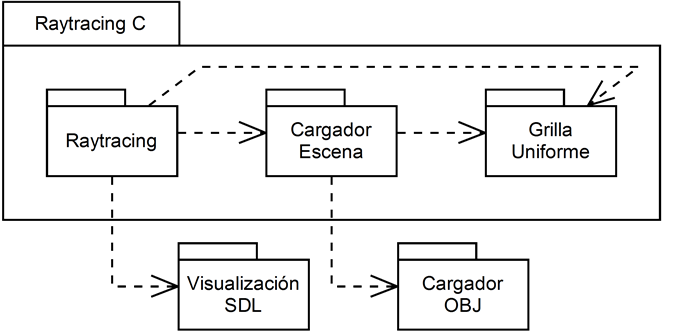
\includegraphics[width=0.8\textwidth]{./Capitulo4/ARQ_RT_C}
    \caption{Arquitectura del Raytracing implementado sobre GPU.}
    \label{fig:ArqRayTracingGPU}
\end{figure}

En primer t�rmino se defini� una arquitectura gen�rica para la soluci�n, en la Figura \ref{fig:ArqRayTracingGPU} se muestra un diagrama de arquitectura de la soluci�n implementada. En lo que resta de la secci�n se detallan las etapas implementadas, se profundiza en las distintas versiones que se desarrollaron, adem�s, se explican las etapas resueltas con otras herramientas.

Los componentes involucrados en la etapa de preprocesamiento son: ``\emph{OBJ Loader}'', ``Cargador Escena'' y ``Grilla Uniforme''. El componente ``\emph{OBJ Loader}'' es el encargado de leer el archivo que especifica la escena y los materiales utilizados en la misma. El componente ``Cargador Escena'' que utiliza el ``\emph{OBJ Loader}'' fue implementado en el marco de este proyecto. Este componente tiene su propia estructura de datos para el almacenamiento de la escena, debido a esto se encarga de inicializar su estructura a partir de los datos le�dos. Adem�s se encarga de la construcci�n de la subdivisi�n espacial uniforme. La divisi�n espacial se genera utilizando el componente ``Grilla Uniforme'', esta parte del sistema construye la grilla a partir de la lista de objetos que contiene el encargado de inicializar la estructura de datos de la escena. Por �ltimo, el componente ``Raytracing'' es el encargado de calcular los rayos primarios utilizado la GPU.

En la segunda etapa del proceso de generaci�n de imagen se calcula el color de cada pixel mediante el algoritmo de Raytracing. Esta etapa se realiza enteramente a nivel de GPU. Hablando en t�rminos de la arquitectura, el componente ``Raytracing'' es el encargado de renderizar la imagen. Dentro de este se implementaron los algoritmos que componen el n�cleo del raytracing, como por ejemplo el algoritmo de recorrida de un rayo dentro de la subdivisi�n espacial uniforme, el algoritmo de intersecci�n rayo-tri�ngulo, etc.

En la �ltima etapa se presenta en pantalla la imagen que surge como resultado de la etapa anterior. Desde el punto de vista de la arquitectura, el componente ``Raytracing'' es el encargado de mostrar la imagen generada utilizando la librer�a externa SDL (Simple Directmedia Layer) \cite{SDLLibrarySite}.

A continuaci�n se presentan los aspectos m�s relevantes del dise�o de la soluci�n implementada.

\subsection{Preprocesamiento}

En este trabajo la escena es cargada desde un archivo de texto usando exclusivamente la CPU. El formato de este archivo esta basado en el Wavefront OBJ version 3.0 \cite{OBJFileFormat}.

Los datos de la escena son cargados en memoria mediante un cargador implementado por Micah Taylor \cite{FuenteCargadorOBJ} llamado \emph{OBJ Loader}. El \emph{OBJ Loader} es capaz de interpretar el formato OBJ completamente, pero tambi�n es capaz de leer otros datos que no son parte del est�ndar de Wavefront, pero que son muy �tiles para el algoritmo de Raytracing. Las caracter�sticas extras soportadas por el \emph{OBJ Loader} y que extienden el formato OBJ son:
\begin{itemize}
    \item soporte de nuevas primitivas, por ejemplo plano.
    \item soporte de elementos extra, como por ejemplo luces puntuales y c�maras.
    \item soporte de propiedades de material avanzadas, como por ejemplo el coeficiente de reflexi�n y el de transmisi�n de un material.
\end{itemize}

El \emph{OBJ Loader} tiene su propia estructura de datos para almacenar la escena en memoria, pero en la propuesta implementada en este proyecto son utilizadas temporalmente. Despu�s de cargar la escena con el \emph{OBJ Loader}, esta se almacena en una estructura definida especialmente. De esta manera se desacopla el resto del algoritmo de la etapa de carga, lo cual permite cambiar f�cilmente la herramienta de carga de la escena.

En la etapa de preprocesamiento se necesitan diferentes par�metros. La resoluci�n de la grilla de aceleraci�n, as� como otros par�metros del algoritmo de raytracing se definen mediante el uso de un archivo de configuraci�n. Se tom� la decisi�n de utilizar un archivo de configuraci�n ya que para las pruebas de rendimiento es interesante cambiar los valores de los par�metros m�s importantes de cada algoritmo y no tener que re-compilar el c�digo fuente con cada cambio. La Figura \ref{fig:EjemploArchivoConfig} se muestra una posible configuraci�n del algoritmo.

\begin{figure}[H]
    \begin{center}
    \begin{boxedverbatim}
TAMANIO_GRILLA.X=64 /*tama�o de la partici�n espacial*/
TAMANIO_GRILLA.Y=50
TAMANIO_GRILLA.Z=50
RESOLUCION.X=640 /*resoluci�n de la imagen*/
RESOLUCION.Y=480
INFINITO= 34028234660000000
ZERO=0.000001 /*valor tomado como cero*/
PROFUNDIDAD_RECURSION=3 /*valor m�ximo rebotes rayo*/
THREADS.X=8 /*hilos por bloque*/
THREADS.Y=16
ESCENA=../escenas/afrodita.obj
    \end{boxedverbatim}
\end{center}
\caption{Ejemplo de contenido para el archivo de configuraci�n.}
\label{fig:EjemploArchivoConfig}
\end{figure}

En el archivo adem�s del tama�o de la subdivisi�n espacial uniforme, se debe indicar el tama�o de la partici�n en cada eje de coordenadas, la resoluci�n de la imagen (en pixeles) que genera el algoritmo de raytracing, valores para el cero y para el infinito que usa el algoritmo (el ajuste del cero permite solucionar problemas de errores num�ricos mientras que el segundo se usa en algoritmos que necesitan definir una distancia ``infinita''). Otro par�metro necesario para el algoritmo de raytracing es la profundidad m�xima considerada por el algoritmo para cada �rbol de rayos. Por �ltimo, se debe especificar la dimensi�n de los bloques de hilos de ejecuci�n.

\subsection{Intersecci�n}

En este proyecto se decidi� acelerar el algoritmo de Raytracing por medio de disminuir el tiempo de ejecuci�n que toman las intersecciones rayo-objeto, pues estas consumen m�s del 90\% del tiempo de generaci�n de imagen \cite{TesisEstructuras}. En este sentido se atacaron los puntos cr�ticos del proceso de intersecci�n rayo-escena: implementar un algoritmo eficiente de intersecci�n rayo-primitiva y reducir la cantidad de intersecciones rayo-primitiva que se prueban por cada rayo primario.

El algoritmo de trazado de rayos implementado �nicamente posee un tipo de primitiva, el tri�ngulo, por lo tanto solo se debi� escoger un m�todo para la intersecci�n rayo-tri�ngulo. Se escogi� �nicamente el tri�ngulo como primitiva de construcci�n de escenas porque es una primitiva sencilla, y a su vez permite construir cualquier objeto tridimensional us�ndola como base. Asimismo, al ser una primitiva b�sica su algoritmo de intersecci�n con un rayo es simple, lo cual implica que se requieran pocas operaciones aritm�ticas para probar su intersecci�n con un rayo. Adem�s, es una primitiva ampliamente soportada por la mayor�a de herramientas de modelado tridimensional, como \emph{3D Studio Max} \cite{3DSMAXWebSite}, \emph{Maya} \cite{MayaWebSite}, \emph{Blender} \cite{BlenderWebSite}, etc.

El m�todo utilizado para verificar la intersecci�n entre un rayo y un tri�ngulo es el de coordenadas baric�ntricas. Dicho m�todo verifica que el rayo interseque con el plano que contiene al tri�ngulo y luego mediante un cambio de coordenadas verifica que la intersecci�n est� dentro de los l�mites del mismo \cite{RealTimeRendering02}. Este m�todo no es el m�s eficiente que existe pero su consumo de memoria es m�nimo, lo cual es importante si se quiere implementar el algoritmo en una GPU.

\subsection{Aceleraci�n espacial}

A pesar de contar con un algoritmo de intersecci�n eficiente es importante implementar una estrategia para no probar para cada rayo primario la intersecci�n con todos los objetos de la escena. En la etapa de relevamiento se evaluaron tres estructuras de aceleraci�n espacial: la subdivisi�n espacial uniforme, la subdivisi�n espacial adaptativa (utilizando Kd-trees) y la jerarqu�a de vol�menes envolventes (BVH), que se describen en el Capitulo \ref{cap:AceleracionRaytracing}.

La estrategia de aceleraci�n espacial que se adopto en este proyecto fue la subdivisi�n espacial uniforme. El argumento de mayor peso para la elecci�n de esta estructura fue la simplicidad de construcci�n y recorrida de la misma, lo cual resulta imprescindible para paralelizar los algoritmos usando una GPU.

\subsubsection{Construcci�n de la grilla}

Para la construcci�n de la grilla se evaluaron dos m�todos. Ambos m�todos se implementaron exclusivamente en la CPU, aunque podr�an ser acelerados ejecut�ndolos en la GPU.

El primer algoritmo implementado fue la construcci�n por fuerza bruta. Como se muestra en el Algoritmo \ref{alg:SeudoConsGrillaBruto}, este m�todo de construcci�n recorre todos los voxels de la grilla y para cada uno de ellos recorre todos los objetos de la escena para probar si hay intersecci�n voxel-objeto. Este m�todo es ineficiente porque por lo general se recorren muchos voxels innecesarios (que no tienen intersecci�n con el objeto) por cada objeto de la escena.

En el Algoritmo \ref{alg:SeudoConsGrillaOptimizado} se describe el segundo algoritmo de construcci�n. Este caso es un algoritmo optimizado donde se recorren todos los objetos de la escena y para cada uno ellos se calcula (en coordenadas de la grilla) una caja alineada a los ejes que lo envuelve. A partir de la caja se obtienen voxels candidatos a solaparse con el objeto. Para cada voxel candidato se prueba el solapamiento caja-objeto y si da positiva se agrega el objeto al voxel que dio origen a la caja. La optimizaci�n introducida con respecto al m�todo mostrado en el Algoritmo \ref{alg:SeudoConsGrillaBruto} permite desechar una cantidad importante de voxels que no tienen intersecci�n con el objeto. Excepto en el peor caso (cuando todos los objetos de la escena se solapan con todos los voxels de la grilla), el m�todo optimizado es m�s eficiente que el original, ya que disminuye la cantidad de pruebas de intersecci�n voxel-objeto.

\begin{algorithm}
    \caption{Pseudoc�digo del algoritmo de fuerza bruta de construcci�n de la grilla uniforme.}
    \label{alg:SeudoConsGrillaBruto}
    \begin{algorithmic}
        \ForAll {voxel en grilla}
            \ForAll {obj en listaObjetos}
                \State //En coordenadas de la grilla
                \State bbObj = calcularBoundingBoxObjeto(obj);
                \If{(voxel $\cap$ bbObj) $\neq$ $\emptyset$}
                    \State agregarObjetoEnVoxel(voxel, obj);
                \EndIf
            \EndFor
        \EndFor
    \end{algorithmic}
\end{algorithm}

\begin{algorithm}
    \caption{Pseudoc�digo del algoritmo eficiente de construcci�n de la grilla uniforme.}
    \label{alg:SeudoConsGrillaOptimizado}
    \begin{algorithmic}
        \ForAll {obj en listaObjetos}
            \State //En coordenadas de grilla
            \State bbObj = calcularBoundingBoxObjeto(obj);
            \ForAll {voxel $\subset$ bbObj}
                \State //En coordenadas de mundo
                \State voxelMundo = transformarCoorMundo(voxel);
                \If{boundingBoxOverlapObject(voxelMundo, obj)}
                    \State agregarObjetoEnVoxel(voxel, obj);
                \EndIf
            \EndFor
        \EndFor
    \end{algorithmic}
\end{algorithm}

\subsubsection{Recorrido de la grilla}

El algoritmo para recorrer la grilla est� basado en el algoritmo de renderizado de una l�nea en pantalla, que se implementa en las GPUs. El recorrido de un rayo a trav�s de la grilla de subdivisi�n espacial genera una lista de voxels, estos voxels son los que el rayo atraviesa sucesivamente. El algoritmo se basa en incrementar de manera inteligente un punto a lo largo del rayo, con cada incremento se avanza al siguiente voxel realizando unas pocas sumas y evaluaciones de condici�n.

La implementaci�n se realiza en 2 pasos, primero se computa el c�lculo del voxel inicial y de los incrementos en cada una de las 3 direcciones para un rayo espec�fico y por otra parte la manera en que se computa cada cambio de voxel. El voxel inicial se calcula de manera sencilla intersecando el rayo con el cubo que acota toda la escena que se utiliza para generar la grilla, con el punto de intersecci�n se calcula cual es el voxel al que pertenece el punto. Para obtener el incremento se calcula la derivada en cada una de las 3 componentes, con esa derivada y el tama�o de los voxels en x, y, z se obtiene la distancia que debe recorrer el rayo para poder alcanzar el siguiente voxel, esta se calcula para cada una de las 3 componentes y se almacena en una variable, as� como tambi�n se hace con las derivadas.

En el Algoritmo \ref{alg:SeudoSiguinteVoxelGrilla} se muestra la forma en que se calcula el siguiente voxel. Este c�lculo est� basado en la distancia que tiene que recorrer el rayo desde su origen hasta el siguiente punto de intersecci�n. Se tienen tres distancias que debe recorrer el rayo para pasar al siguiente voxel en el eje X, para pasar al siguiente voxel en el eje Y y para pasar al siguiente voxel en el eje Z. La m�nima de estas distancias determina cual de los tres incrementos es el que hay que realizar, el voxel que est� m�s cerca es el siguiente, por lo tanto hay que incrementar 1 en la direcci�n determinada por dicho m�nimo.

\begin{algorithm}[H]
    \caption{Pseudoc�digo del algoritmo para avanzar en los voxels.}
    \label{alg:SeudoSiguinteVoxelGrilla}
    \begin{algorithmic}
        \If{(Minimo(DX, DY, DZ) == DX)}
            \State DX = DX + incrementoX;
            \State VoxelActualX = VoxelActualX + signo(incrementoX) * 1;
        \EndIf
        \If{(Minimo(DX, DY, DZ) == DY)}
            \State DY = DY + incrementoY;
            \State VoxelActualY = VoxelActualY + signo(incrementoY) * 1;
        \EndIf
        \If{(Minimo(DX, DY, DZ) == DZ)}
            \State DZ = DZ + incrementoZ;
            \State VoxelActualZ = VoxelActualZ + signo(incrementoZ) * 1;
        \EndIf
    \end{algorithmic}
\end{algorithm}

\subsection{N�cleo de Raytracing sobre GPUs}

Considerando la arquitectura del sistema, el n�cleo principal del Raytracing para GPU se encuentra implementado dentro del componente ``Raytracing''. Para lograr que el algoritmo tenga un buen rendimiento es necesario utilizar adecuadamente la jerarqu�a de memoria de la GPU. Los datos m�s utilizados por el algoritmo, como por ejemplo la lista de objetos de la escena o los voxeles de la subdivisi�n espacial, deben estar almacenados en un tipo de memoria que tenga tiempo de lectura bajo, y pudiendo ser de solo lectura, ya que esta informaci�n es frecuentemente accedida y nunca debe ser actualizada. Es por ello que la lista de tri�ngulos y sus normales, las luces, los voxeles de la grilla de subdivisi�n espacial y la lista de materiales se copian a la memoria de textura de la GPU. Otra informaci�n como los datos de la c�mara, la cantidad de luces, la dimensi�n de la grilla se copian a la memoria constante de la GPU, que tambi�n es de solo lectura. La lectura en los dos tipos de memoria mencionados es mucho m�s r�pida que una lectura en memoria global.

El uso de la jerarqu�a de memoria que provee CUDA afecta directamente a la estructura de datos que almacena la escena. Por ejemplo, la lista de tri�ngulos de la escena ocupa una cantidad grande de memoria y al cargarla desde archivo insume un tiempo de ejecuci�n considerable. Toma pr�cticamente el mismo tiempo transformar toda la lista de tri�ngulos desde el formato en que esta almacenada hacia el formato que requiere CUDA para cargarla en memoria de textura. Es por esto que se decidi� almacenarla directamente en el formato que debe tener para copiarla a memoria de la GPU (ver Ap�ndice \ref{sec:ApendiceEstructurasDatos}).

En la memoria de textura solo se pueden copiar vectores de dos o cuatro elementos, debido a esto cada v�rtice de tri�ngulo se almacena como un vector de cuatro componentes, desperdiciando una componente (4 bytes) por cada v�rtice. En algunos casos se aprovecha la memoria de la cuarta componente, por ejemplo el identificador de material se guarda en la cuarta componente del primer v�rtice de cada tri�ngulo. De todas formas para usar la jerarqu�a de memoria y mejorar el tiempo de ejecuci�n del algoritmo se pierde la generalidad en las estructuras de datos y la legibilidad del c�digo fuente.

Una vez copiados todos los datos de entrada del algoritmo de Raytracing a la GPU, se procede a la invocaci�n del \emph{kernel} encargado de calcular los rayos primarios. Como se muestra en la Figura \ref{fig:DiagramaRTGPU}, los datos necesarios para calcular los rayos primarios son: el plano de vista, la c�mara y la resoluci�n de la imagen a renderizar. Toda esta informaci�n se encuentra en memoria constante y puede ser accedida en cualquier instante del tiempo de vida de la aplicaci�n CUDA. Es importante resaltar que la invocaci�n al \emph{kernel} que calcula rayos se hace desde la CPU y cuando este finaliza su procesamiento retorna nuevamente a la CPU.

Los rayos primarios son datos de entrada para el \emph{kernel} encargado de calcular el color de cada pixel. Inmediatamente despu�s que se tienen calculados los rayos primarios, se invoca el \emph{kernel} (desde la CPU) que genera la imagen. Dentro de este se encuentra implementado el coraz�n del algoritmo de raytracing. Los datos de entrada necesarios para calcular el color de cada pixel se muestran en la Figura \ref{fig:DiagramaRTGPU} y son le�dos desde memoria de textura, cuyo tiempo de vida es igual al de la aplicaci�n CUDA.

El \emph{kernel} principal es invocado seg�n una divisi�n en parches (conjunto de pixeles) de la imagen a generar, tal como se detalla en la Secci�n \ref{sec:ParalelizacionAlgoritmo}. De esta forma, cada parche es asociado con un bloque de ejecuci�n de CUDA y la cantidad de hilos que ejecutan el procedimiento de c�lculo de color es igual a la cantidad de pixeles. Cada uno de los rayos lanzados recorrer� la estructura de aceleraci�n espacial, siguiendo los reflejos y refracciones. Al finalizar esta ejecuci�n es que se realiza la copia de los datos generados en la GPU nuevamente a la CPU para ser mostrados en pantalla.

\begin{figure}[H]
    \centering
        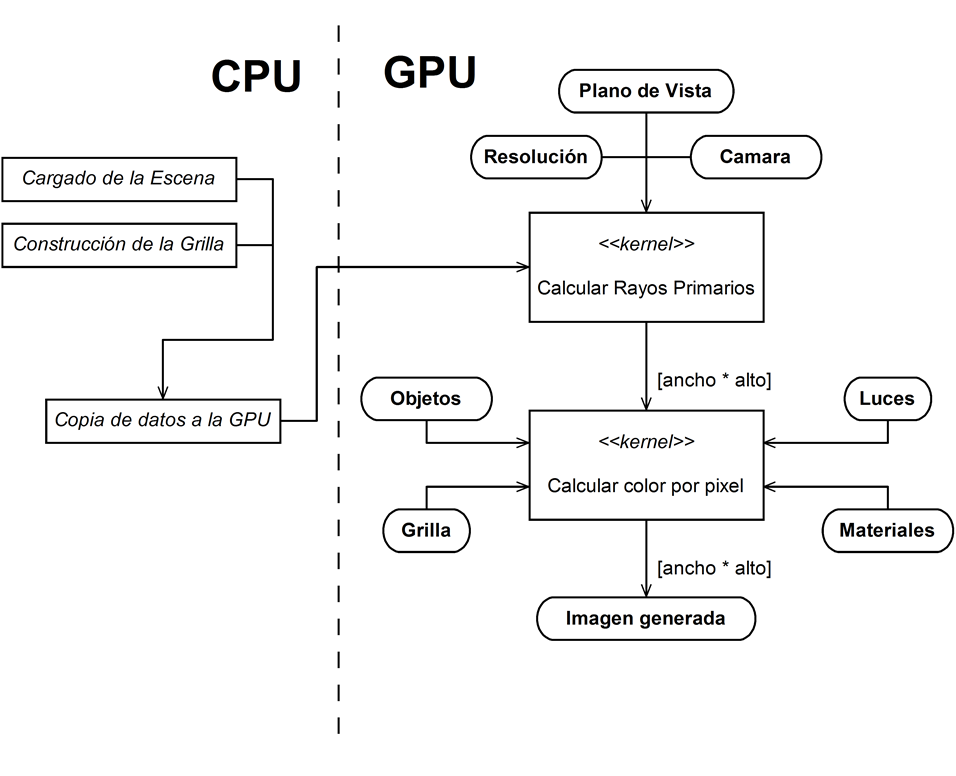
\includegraphics[width=0.8\textwidth]{./Capitulo4/diagramaRT_GPU}
    \caption{Estructura del algoritmo de raytracing implementado en CUDA.}
    \label{fig:DiagramaRTGPU}
\end{figure}

\subsection{Paralelizaci�n del algoritmo}\label{sec:ParalelizacionAlgoritmo}

Para resolver el problema en t�rminos del modelo de programaci�n usado por CUDA se hizo una descomposici�n en sub-problemas, dividiendo la imagen a renderizar. La imagen se divide usando una grilla uniforme de dos dimensiones, donde cada celda de la grilla tiene la misma cantidad de pixeles. En la Figura \ref{fig:subfigDivisionImagen:a} se muestra una posible divisi�n de la imagen. En este ejemplo la imagen se divide en $n \times m$ celdas, quedando as� cada celda con $\frac{R_{x}}{n}\times\frac{R_{y}}{m}$ pixeles. En la Figura \ref{fig:subfigDivisionImagen:b} se muestra en detalle la celda definida por los intervalos $[X_{i},X_{i+1}]$ y $[Y_{j},Y_{j+1}]$, la cual contiene una peque�a parte de los pixeles de la imagen. Cada celda de la grilla se corresponde directamente con un bloque de hilos de ejecuci�n de CUDA, es decir cada divisi�n de la imagen es procesada por un bloque de CUDA diferente. Adem�s, como cada pixel de la imagen es procesado por un hilo de ejecuci�n diferente, la cantidad de hilos por bloque es igual a la cantidad de pixeles que contiene cada divisi�n. Es por esta raz�n que la partici�n queda totalmente establecida cuando se fija la cantidad de hilos de ejecuci�n por bloque (en el archivo de configuraci�n), adem�s de la resoluci�n de la imagen a renderizar. Si se tiene una resoluci�n de imagen de $640\times480$ pixeles y el tama�o de los bloques es de $16\times8$ hilos la imagen es dividida en una grilla de $40\times60$ celdas.

\begin{figure}[H]
    \centering
    \subfigure[]{
        \label{fig:subfigDivisionImagen:a} %% label for first subfigure
        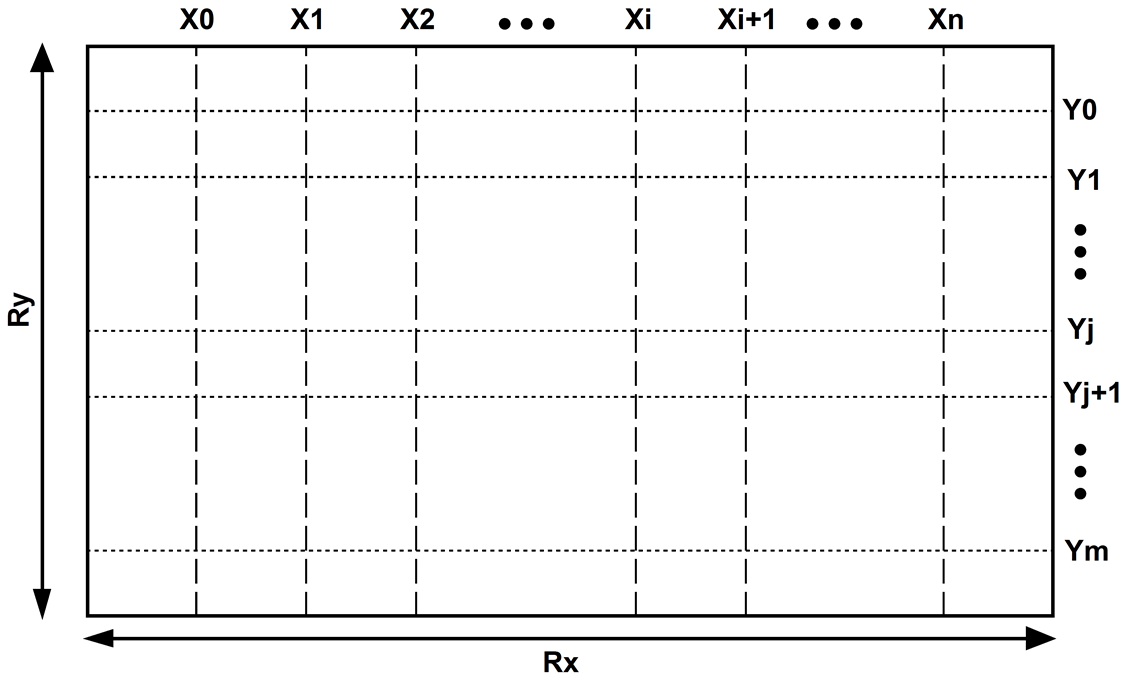
\includegraphics[width=0.45\textwidth]{./Capitulo4/divisionImagen}}
    \subfigure[]{
        \label{fig:subfigDivisionImagen:b} %% label for second subfigure
        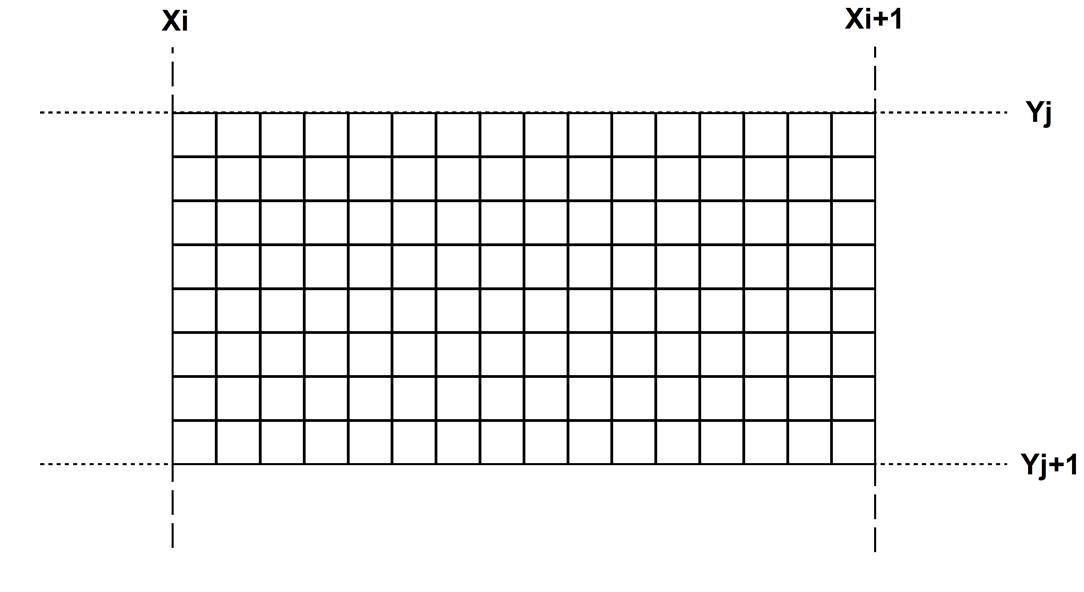
\includegraphics[width=0.45\textwidth]{./Capitulo4/divisionBloque}}
    \caption{Subdivision de la imagen para lograr paralelismo.}
    \label{fig:subfigDivisionImagen} %% label for entire figure
\end{figure}

Mediante esta forma de descomponer el problema el raytracing para CUDA puede escalar f�cilmente en el n�mero de procesadores de la GPU sin necesidad de recompilar su c�digo fuente. Adem�s mediante el archivo de configuraci�n es posible cambiar la partici�n de la imagen a renderizar de manera de optimizarla para cualquier GPU.

La cantidad m�xima de hilos de ejecuci�n por bloque es $512$, por consiguiente $512$ es la cantidad m�xima de pixels que pueden ser procesados por un mismo bloque, limite impuesto por CUDA (versi�n 2.3). Tambi�n hay que tener en cuenta que la cantidad de hilos por bloque puede verse limitada por la cantidad de registros que consuma cada hilo, ya que por ejemplo la cantidad m�xima de registros por bloque es $8192$ (CUDA versi�n 2.3).


\subsection{Eliminaci�n de la recursi�n}

El algoritmo de Raytracing es un algoritmo inherentemente recursivo, esto es una limitaci�n a la hora de hacer que se ejecute en la GPU dado que la ejecuci�n debe ser secuencial, ya que CUDA no tiene soporte para recursi�n. Este algoritmo puede analizarse como una recorrida en un �rbol binario (el �rbol de rayos originado por un rayo primario y sus sucesivos rebotes debido a los fen�menos de reflexi�n y refracci�n).

Para resolver este problema se evaluaron dos opciones, la primera consiste en implementar una pila la cual sirva de apoyo para la recorrida del �rbol binario. La segunda consiste en simplificar el �rbol de manera que degenere en una lista, esta forma de simplificar el �rbol implica una pre-condici�n sobre la escena de entrada, que en la escena no existan objetos que reflejen y transmitan la luz al mismo tiempo.

La opci�n elegida fue la segunda ya que simplifica el algoritmo a implementar en la GPU a cambio de incluir una limitaci�n aceptable a nivel de las escenas de entrada. Otra raz�n importante para optar por simplificar el �rbol de rayos, es que en caso de implementar la primer opci�n cada hilo de ejecuci�n debe contar con una pila y la cantidad de memoria local de cada hilo de ejecuci�n de CUDA es muy limitada.

Para implementar el algoritmo simplificado e iterativo se modific� el original, de forma que cada rayo sea el encargado de llevar el estado de su trayectoria de manera iterativa. En caso de que el rayo interseque con alg�n objeto cuyo material posea reflexi�n o refracci�n, se debe modificar la direcci�n del mismo seg�n las propiedades del material, para que en la siguiente iteraci�n se trace en la trayectoria correcta. Mientras el rayo siga rebotando en los objetos de la escena y no se supere la cantidad m�xima de rebotes se debe continuar con este proceso iterativo.

\subsection{Estructura de datos}
Durante el proyecto se desarrollaron diferentes estructuras de datos para trabajar en GPU, las cuales se muestran en detalle en el Ap�ndice \ref{sec:ApendiceEstructurasDatos}. A continuaci�n se presentan las principales caracter�sticas de las estructuras de datos utilizadas.

La primera versi�n de la estructura de datos usada para trabajar en GPU busca almacenar los datos de la escena de forma ``prolija''. Entre los principios de su concepci�n se encuentran: sencillez de acceso a los datos al momento de implementar los algoritmos, simple introducci�n de nuevos tipos de primitivas y uso eficiente de memoria del sistema.

Entre los campos m�s importantes de la estructura utilizada para almacenar la escena se encuentra la lista de objetos de la misma, que se guardan en un arreglo (\emph{objetos}) con tope (\emph{cant\_objetos}). Otro campo importante donde se guarda la informaci�n referente a la divisi�n espacial de la escena, es el campo \emph{grilla}, que es a su vez otra estructura de datos llamada \emph{UniformGrid}. Esta estructura tiene varios campos:
\begin{itemize}
    \item \emph{dimension}: almacena la dimensi�n de la grilla que divide el espacio de la escena.
    \item \emph{bbEscena}: almacena una caja alineada a los ejes de coordenadas que contiene a toda la escena.
    \item \emph{voxels}: array de punteros a entradas de \emph{listasGrid}. Cada entrada de \emph{voxels} se corresponde con un voxel de la escena, donde se almacena un puntero a la lista de objetos que contiene el voxel.
    \item \emph{listasGrid}: array de listas de punteros a objetos.
\end{itemize}

Se puede ver un ejemplo esquem�tico de la estructura \emph{UniformGrid} en la Figura \ref{fig:exampleEstructuraUGrid}. En este ejemplo se considera una escena con seis objetos, los cuales est�n completamente contenidos es una caja alineada a los ejes definida por los puntos $min = (-10, -10, -10)$ y $max = (10, 10, 10)$. Al aplicarle una subdivisi�n espacial uniforme con dimensiones $2\times2\times3$ a la escena se generan $12$ voxels, tal como se muestra en el vector ``voxels''. Cada objeto de la escena se encuentra contenido en una o m�s divisiones, por lo tanto por cada divisi�n se tiene una lista de objetos contenidos. El vector ``listasGrid'' contiene las listas de todos los voxels de la subdivisi�n y mediante las entradas del vector ``voxels'' se accede a cada una de ellas. El caso especial en que la lista de objetos de un voxel es vac�a se marca con un valor especial en el vector ``voxels''.

\begin{figure}[H]
  \centering
    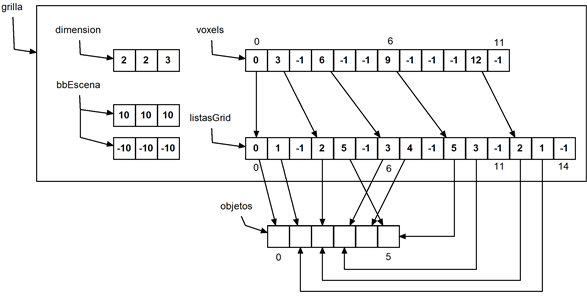
\includegraphics[width=0.8\textwidth]{./../DOC_Implementacion/estructuraGrilla}
  \caption{Ejemplo de estructura \emph{UniformGrid}.}
  \label{fig:exampleEstructuraUGrid}
\end{figure}


La segunda versi�n de la estructura de datos usada para trabajar en GPU es una evoluci�n de la primera. Los cambios que generaron la evoluci�n estuvieron determinados por la forma de utilizar la jerarqu�a de memoria de la GPU. La estructura tuvo que ser reordenada de manera de minimizar las operaciones de memoria al momento de cargar los datos de la escena en la GPU. Lo que m�s afecta la eficiencia es reordenar los datos antes de cargarlos en memoria de textura de la GPU. Es importante que el copiado de memoria de la CPU hacia la GPU sea lo m�s eficiente posible ya que de esta manera se reduce el tiempo de ejecuci�n consumido por la etapa de preprocesamiento.

Los campos m�s importantes de la segunda versi�n de la estructura son los mismos que en la primera versi�n, ya que s�lo se ordenaron de manera diferente. El �nico campo importante que se modific� fue la lista de objetos, se paso de almacenar una lista agrupada por objetos (lista de pares v�rtices-normales) a almacenar varias listas, una por cada propiedad de los objetos (una lista de v�rtices y otra de normales).

Otra diferencia importante entre la primera y la segunda versi�n es que en la segunda algunos tipos de datos se modificaron para adaptarlos a los tipos de datos soportados por la jerarqu�a de memoria de CUDA. Por ejemplo, en la primera versi�n la lista de luces es una lista de \emph{float3}, donde los primeros dos definen la posici�n y el color de la primer luz respectivamente, los segundos dos la posici�n y el color de la segunda y as� sucesivamente. Como la lista de luces se carga en memoria de textura y la memoria de textura no permite cargar vectores de tres componentes, en la segunda versi�n se opt� por transformar la colecci�n de luces en una lista de \emph{float4}, donde cada propiedad es definida utilizando �nicamente las primeras tres componentes.

\section{Versiones implementadas}
El desarrollo del Raytracing para CUDA fue iterativo-incremental, desarrollando tres grandes versiones. En forma general la primera versi�n implementa el Raytracing de Whitted completo, la segunda versi�n esta marcada por la introducci�n de mejoras que tienen que ver con la optimizaci�n en la explotaci�n de la jerarqu�a de memoria de la GPU. Por �ltimo, la tercera est� se�alada por la mejora del algoritmo de c�lculo de la intersecci�n rayo-tri�ngulo.

\subsection{Versi�n 1: RT-GPU}
Las principales caracteristicas de esta versi�n son:
\begin{itemize}
    \item Implementa el algoritmo de Whitted con reflexi�n y refracci�n de forma iterativa.
    \item Utiliza la estructura de aceleraci�n espacial \emph{Uniform Grid}.
    \item La generaci�n de rayos primarios se hace en un \emph{kernel} de CUDA.
    \item Para la recorrida de la grilla, el trazado de rayos de sombra y secundarios se utiliza un s�lo \emph{kernel} de CUDA.
    \item Las operaciones sobre vectores se hacen usando las operaciones propias de CUDA.
\end{itemize}
Las principales restricciones de la versi�n RT-GPU son:
\begin{itemize}
    \item las escenas deben tener como m�ximo una luz puntual.
    \item las escenas no pueden tener objetos reflexivos y transparentes a la vez.
    \item la sombra proyectada por un objeto transparente no tiene en cuenta el color del objeto.
    \item no se explota al m�ximo la estructura de memoria de la GPU.
    \item sufre el problema que genera el sistema operativo al ejecutar un \emph{kernel} por m�s de 5 segundos. El sistema operativo impone que un \emph{kernel} puede ejecutar como m�ximo por 5 segundos, en caso de que se exceda este tiempo el sistema operativo reinicia el \emph{driver} de video al considerar que este se encuentra inactivo, cancelando la ejecuci�n del \emph{kernel}.
\end{itemize}

\subsection{Versi�n 2: RT-GPU-JM}
Esta versi�n presenta las mismas caracter�sticas que RT-GPU y elimina la restricci�n ``no explota al m�ximo la estructura de memoria de la GPU'', usando la jerarqu�a de memoria (memoria de textura y constante principalmente) para almacenar las estructuras de datos que representan la escena a procesar por el algoritmo.

\subsection{Versi�n 3: RT-GPU-JM-IR}
Esta versi�n presenta las mismas caracter�sticas que RT-GPU-JM y modifica el algoritmo de intersecci�n rayo-tri�ngulo para disminuir el tiempo de ejecuci�n de cada test de intersecci�n.

\subsection{Versiones para CPU}
Para cada versi�n desarrollada del Raytracing sobre GPU se implement� una versi�n similar en cuanto a las cualidades de optimizaci�n para ejecutarla sobre CPU. De esta manera se dispone de versiones de referencia sobre arquitecturas tradicionales para comparar el desempe�o. 
\chapter{Experimentaci�n} % 20 p�ginas mas o menos...

\section{Relevamiento calidad imagen}

Para evaluar la correcci�n de la soluci�n implementada es necesario, adem�s de una evaluaci�n de la velocidad de generaci�n de las im�genes, una medida de la calidad de las mismas. Por eso es que se relev� en el campo de la generaci�n de im�genes cu�les eran los m�todos con los que se evaluaba la calidad de los generadores de im�genes m�s importantes. En esta investigaci�n no se pudieron encontrar estrategias solidas para evaluar la calidad. A continuaci�n se describen a grandes rasgos los algoritmos que existen para la evaluaci�n de calidad de im�genes.




Se realiz� una categorizaci�n de las medidas de evaluaci�n de calidad, basada en el articulo de Ismail Avcibas y B�lent Sankur \cite{QualityMeasuresCategories} y analizando el resto de la informaci�n disponible \cite{HVSQualityAssessment} \cite{IdentifyingComputerGeneratedImages} \cite{SegmentationPerceptualImageQualityAssessment} \cite{StructuralSimilarityPerceptualImageQualityAssessment}. Cabe se�alar que si bien el art�culo \cite{QualityMeasuresCategories} no es sobre la generaci�n de im�genes, se pueden ver ciertas similitudes en los objetivos de todas y cada una de las medidas de calidad de im�genes.
Las categor�as en las que se dividen los algoritmos de evaluaci�n de calidad son:
Basados en diferencias a nivel de p�xeles, basados en correlaci�n, basados en aristas, basados en an�lisis espectral, basados en contexto y basados en el sistema visual humano (HVS por su sigla en ingl�s).

Las estrategias basadas en diferencias a nivel de p�xeles son los m�s simples, calculan la diferencia entre 2 im�genes tomando como referencia que un pixel en una imagen se corresponde con el mismo pixel de la imagen objetivo y, dependiendo de cu�l de los algoritmos se trate, calcula alguna ponderaci�n de los pixeles para retornar un valor que indicar� la diferencia que hay entre ambas im�genes, la generada y la imagen objetivo.
Las estrategias basads en correlaci�n son muy similares a los anteriores pero pueden introducir una nueva variable: los p�xeles se pueden mover y no estar en el mismo lugar en ambas im�genes. Este tipo de algoritmos son �tiles en muchos casos para el �rea de procesamiento de imagen, en especial porque una misma imagen puede ser generada vista de distintos �ngulos y en el an�lisis de calidad de las mismas considerar que no tienen diferencias.
Otra opci�n se basa en que las im�genes en general presentan en su composici�n aristas que son los bordes que separan los componentes de la imagen entre  si, estas aristas se pueden utilizar para el an�lisis de calidad de imagen. Esta t�cnica se basa en que si dos im�genes son generadas para la misma escena, entonces las im�genes en la imagen ideal que ser�a el objetivo, entonces tambi�n se deben presentar en la imagen generada.
Las estrategias que se basan en el an�lisis espectral son particularmente �tiles en el an�lisis de algoritmos de compresi�n en los que se da este tipo de distorsi�n. Miden la distorsi�n en fase y magnitud, esto pertenece al �rea de tratamiento de se�ales, base del tratamiento de im�genes, pero tampoco se ve una aplicaci�n directa a este trabajo.
En el an�lisis de contexto para medir la calidad de imagen se analiza para cada pixel sus vecinos en una cantidad de niveles arbitraria. Estos p�xeles en caso de que difieran de alguna manera (esto var�a para cada algoritmo dentro de la familia) modificaran, no solo la calidad de ellos mismos como analizan las estrategias de diferencia por pixel, sino tambi�n la calidad de los vecinos, dado que no ser� lo mismo, por ejemplo, un pixel negro entre p�xeles rojos que un pixel negro entre p�xeles blancos.
Por �ltimo, los m�todos basados en el an�lisis de la percepci�n humana para brindar una medida de calidad de la imagen generada. Este tipo de estrategias utilizan los modelos que se han generado para la percepci�n del ojo humano declarando que dos im�genes son iguales si para la percepci�n del ojo humano no tienen diferencias. Este es un modelo razonable en muchos aspectos, en particular para la industria audiovisual, por ejemplo pel�culas, videojuegos, generaci�n de im�genes fotorealistas, entre otras.


Como se puede ver, todas estas estrategias son por ejemplo para comparar im�genes y no lo que realmente interesa en el contexto de este proyecto que es evaluar la calidad de las im�genes generadas por un algoritmo.
En evaluaci�n de im�genes generadas es que se basa el art�culo del a�o 2007 \cite{IdentifyingComputerGeneratedImages}. Claro que plantea, al contrario de lo que se requiere en este caso, detectar que im�genes son generadas por un algoritmo de generaci�n de im�genes y cuales son im�genes reales tomadas con una c�mara. Aunque el objetivo que persigue este art�culo es muy similar al que se persigue en el an�lisis de esta secci�n, el algoritmo propuesto e implementado no cumple con ser fotorealista dado que el modelo utilizado, Raytracing, no es un modelo tan preciso. Por esto es que no se podr�an utilizar los m�todos propuestos en el art�culo.
Por otro lado los algoritmos basados en las capacidades de percepci�n del sistema visual humano en general tambi�n apuntan a evaluar que im�genes son iguales para el ojo humano. Al igual que en el caso anterior, estas estrategias no aplicar�an en el contexto que se requiere. En este caso, por lo tanto, no son aplicables las medidas relevadas para la evaluaci�n de calidad de las im�genes generadas. Si bien se entiende que este podr�a ser un tema de estudio interesante.

\section{Casos de prueba}

Para probar el rendimiento del algoritmo de generaci�n de im�genes implementado es necesario generar escenas a renderizar. Como se ha mencionado en la descripci�n del algoritmo una escena se especifica mediante dos archivos que siguen un formato establecido.

Al momento de dise�ar los casos de prueba para el algoritmo de Raytracing se busco cubrir los aspectos cr�ticos del algoritmo. Un aspecto importante a tener en cuenta es que el algoritmo de Raytracing implementado usa una grilla uniforme como estructura de aceleraci�n. Como se analiz� en la etapa de relevamiento del proyecto este tipo de estructura no es buena cuando la escena tiene una distribuci�n espacial no uniforme de sus elementos. Por ello resulta importante probar el mismo con un conjunto de escenas que mantengan fija la cantidad de objetos, pero que var�en la distribuci�n de ellos.

La cantidad de objetos de la escena es un aspecto que afecta directamente el tiempo de ejecuci�n de un algoritmo de Raytracing. Por este motivo es importante verificar el tiempo de ejecuci�n del algoritmo implementado con escenas que tengan distinta cantidad de objetos pero que mantengan fijas todas las dem�s propiedades.

La comparaci�n con implementaciones similares es importante para establecer la calidad del algoritmo de Raytracing desarrollado en el marco de este proyecto. Por este motivo se incluyen dentro de los casos de prueba escenas pertenecientes a la comunidad web de Raytracing. Dentro de esta clase de escenas externas al proyecto, hay escenas usadas en todo proyecto de generaci�n de im�genes, por ejemplo ``\emph{stanford bunny}'' y tambi�n hay escenas �nicas de proyectos particulares.

Es importante decir que es dif�cil encontrar un algoritmo similar al implementado ya que existen numerosas variantes del mismo, se pueden encontrar diversas t�cnicas de aceleraci�n del algoritmo, entre otros aspectos. Los datos comparables entre las distintas implementaciones son los frames por segundo (FPS), la calidad de la imagen generada, etc.

\subsubsection{Distribuci�n de los objetos en la escena}

Para verificar el comportamiento del algoritmo implementado frente a la uniformidad espacial de los objetos de la escena se dise�aron tres casos de prueba. Como se muestra en la Figura \ref{fig:CPDistrEspacial} los tres casos son similares, la �nica diferencia entre ellos es la posici�n de los objetos (cada uno esta compuesto por 1148 tri�ngulos) en la escena.

\begin{figure}
    \centering
    \subfigure[]{
        \label{fig:CPDistrEspacial:a} %% label for first subfigure
        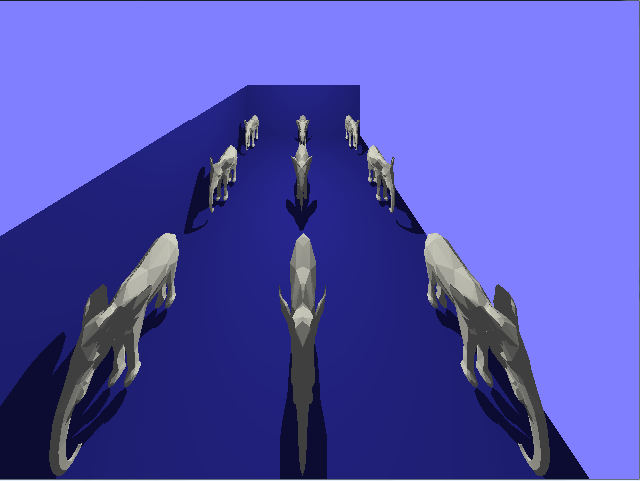
\includegraphics[width=0.3\textwidth]{./Capitulo5/DIST_I}
    }
    \subfigure[]{
        \label{fig:CPDistrEspacial:b} %% label for second subfigure
        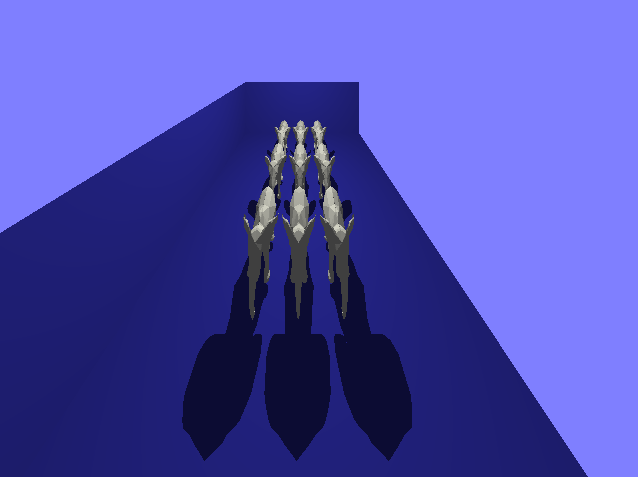
\includegraphics[width=0.3\textwidth]{./Capitulo5/DIST_II}
    }
    \subfigure[]{
        \label{fig:CPDistrEspacial:c} %% label for second subfigure
        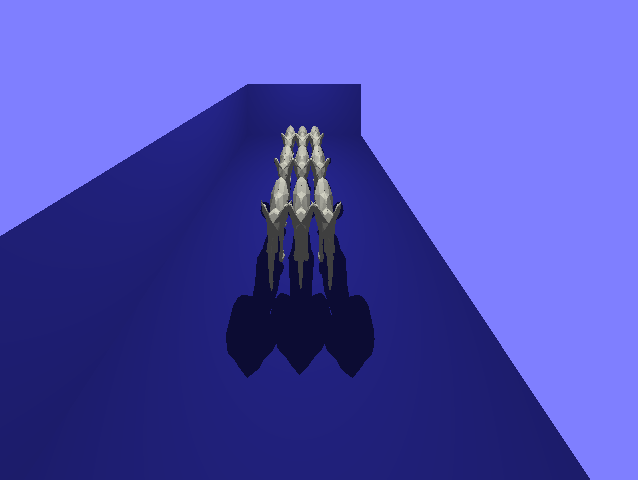
\includegraphics[width=0.3\textwidth]{./Capitulo5/DIST_III}
    }
    \caption{Escenas con distinta disposici�n espacial de los objetos.}
    \label{fig:CPDistrEspacial} %% label for entire figure
\end{figure}

En la Tabla \ref{table:CPDistrEspacial} se muestran algunas caracter�sticas importantes de estos casos de prueba, en especial en la primer columna se muestra una referencia que ser� usada de aqu� en m�s.

\begin{table}[!hbt]
\begin{center}
\resizebox{10cm}{!}{
    \small {
    \begin{tabular}{|c|c|c|c|c|c|}
    \hline
    Ref & Objetos & Luces & Tri�ngulos & Archivo & Imagen\\
    \hline
    DIDT\_I & 9 & 1 & 10338 & elefantesChicosDistUniforme.obj & \ref{fig:CPDistrEspacial:a}\\
    \hline
    DIDT\_II & 9 & 1 & 10338 & elefantesChicosDistNoUniforme.obj & \ref{fig:CPDistrEspacial:b}\\
    \hline
    DIDT\_III & 9 & 1 & 10338 & elefantesChicosDistNoUniformeSOLAP.obj & \ref{fig:CPDistrEspacial:c}\\
    \hline
    \end{tabular}
    }
}
\caption{Datos de entrada para pruebas de distribuci�n.}
\label{table:CPDistrEspacial}
\end{center}
\end{table}


\subsubsection{Cantidad de primitivas de la escena}

Para verificar el comportamiento del algoritmo implementado frente a la cantidad de objetos de la escena de entrada se dise�aron cinco casos de prueba. Los cinco casos de prueba definen la misma escena, la �nica propiedad que cambia entre uno o otro es la cantidad de primitivas (tri�ngulos) usadas para construir los objetos de la misma. Como se muestra en las Figuras \ref{fig:CPCantidadPrimitivas:a} y \ref{fig:CPCantidadPrimitivas:b} cada escena contiene una esfera y un cubo, y existe una diferencia entre las im�genes generadas dada por la variaci�n de la cantidad de tri�ngulos.

\begin{figure}
    \centering
    \subfigure[]{
        \label{fig:CPCantidadPrimitivas:a} %% label for first subfigure
        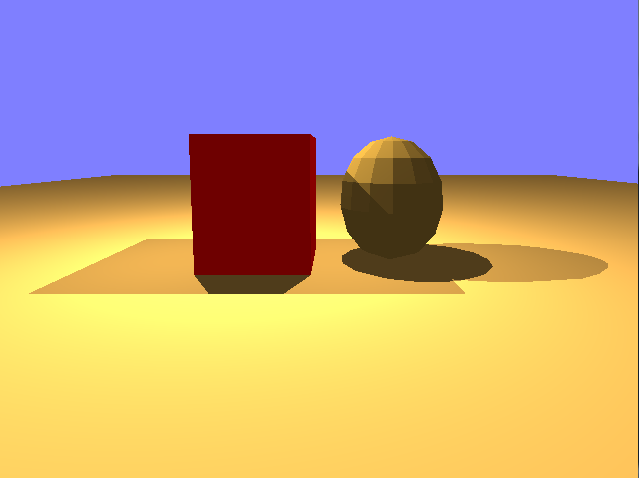
\includegraphics[width=0.3\textwidth]{./Capitulo5/PRI_I}
    }
    \subfigure[]{
        \label{fig:CPCantidadPrimitivas:b} %% label for second subfigure
        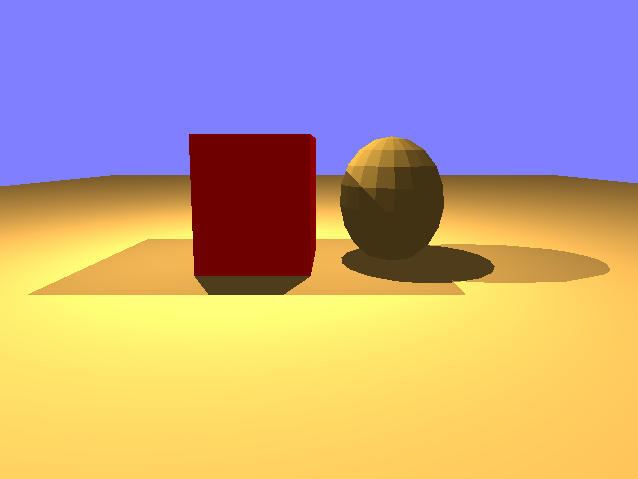
\includegraphics[width=0.3\textwidth]{./Capitulo5/PRI_V}
    }
    \caption{Im�genes de los casos de prueba de cantidad de primitivas.}
    \label{fig:CPCantidadPrimitivas} %% label for entire figure
\end{figure}

En la Tabla \ref{table:CPCantPrimitivas} se muestran algunas caracter�sticas importantes de estos casos de prueba, en especial en la primer columna se muestra una referencia que ser� usada de aqu� en m�s.

\begin{table}[!hbt]
\begin{center}
\resizebox{10cm}{!}{
    \small {
    \begin{tabular}{|c|c|c|c|c|c|}
    \hline
    Ref & Objetos & Luces & Tri�ngulos & Archivo & Imagen\\
    \hline
    PRI\_I & 2 & 2 & 194 & cajaEsfera1.obj & \ref{fig:CPCantidadPrimitivas:a}\\
    \hline
    PRI\_II & 2 & 2 & 274 & cajaEsfera2.obj & -\\
    \hline
    PRI\_III & 2 & 2 & 348 & cajaEsfera3.obj & -\\
    \hline
    PRI\_IV & 2 & 2 & 482 & cajaEsfera4.obj & -\\
    \hline
    PRI\_V & 2 & 2 & 606 & cajaEsfera5.obj & \ref{fig:CPCantidadPrimitivas:b}\\
    \hline
    \end{tabular}
    }
}
\caption{Datos de entrada para pruebas de cantidad de primitivas.}
\label{table:CPCantPrimitivas}
\end{center}
\end{table}



\subsubsection{Comparando con otras implementaciones}

Para la evaluaci�n de la calidad del algoritmo implementado en el marco de este proyecto, resulta imprescindible la comparaci�n con otros algoritmos de Raytracing similares. Por ello se buscaron algoritmos que se ajustaran al modelo de Whitted, implementados sobre CUDA por la comunidad mundial de Raytracing.

\begin{figure}
    \centering
    \subfigure[]{
        \label{fig:CPTerceros:a} %% label for first subfigure
        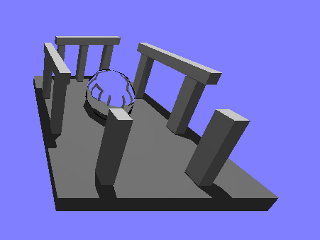
\includegraphics[width=0.2\textwidth]{./Capitulo5/alexandra}
    }
    \subfigure[]{
        \label{fig:CPTerceros:b} %% label for second subfigure
        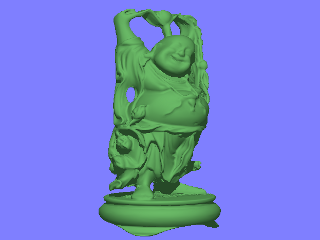
\includegraphics[width=0.2\textwidth]{./Capitulo5/buddha}
    }
    \subfigure[]{
        \label{fig:CPTerceros:c} %% label for second subfigure
        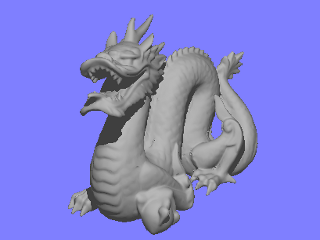
\includegraphics[width=0.2\textwidth]{./Capitulo5/dragon}
    }
    \subfigure[]{
        \label{fig:CPTerceros:d} %% label for second subfigure
        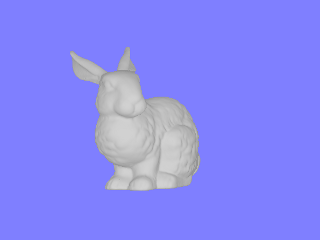
\includegraphics[width=0.2\textwidth]{./Capitulo5/StanfordBunny}
    }
    \caption{Im�genes de los casos de prueba de cantidad de primitivas.}
    \label{fig:CPTerceros} %% label for entire figure
\end{figure}

Los integrantes del grupo de Computaci�n Gr�fica del \emph{Alexandra Institute} de Dinamarca implementaron un algoritmo de Raytracing y se encuentra publicado en su p�gina web \cite{BlogAlexandraInst}. Este algoritmo no permite cambiar la escena que renderiza de forma sencilla, ya que su cargador de escena es distinto al que se usa en este proyecto. Como se dispone de informaci�n (cantidad de tri�ngulos de cada uno de los elementos) sobre la escena del algoritmo del \emph{Alexandra Institute}, se decidi� replicar manualmente dicha escena en el formato que usa el algoritmo implementado en este proyecto. Esta escena esta formada por un conjunto de 13 cajas y una esfera como se muestra en la Figura \ref{fig:CPTerceros:a}. Cada caja tiene 2 tri�ngulos por cara y la esfera tiene 80 caras, por lo tanto la escena completa tiene 236 tri�ngulos. Al renderizar su escena el Raytracing sobre GPU del \emph{Alexandra Institute} logra 13 \emph{frames} por segundo (FPS).

Las escenas cuyos renders se muestran en las Figuras \ref{fig:CPTerceros:b}, \ref{fig:CPTerceros:c} y \ref{fig:CPTerceros:d}, se encuentran dentro de las escenas cl�sicas de todo proyecto de ge\-ne\-ra\-ci�n de im�genes. Contar con estas escenas dentro de los casos de prueba de este proyecto es muy importante porque permite comparar con otros proyectos similares. Adem�s el hecho de que el algoritmo implementado en este proyecto soporte este tipo de casos de prueba, que por lo general se componen de una cantidad importante (100.000) de primitivas, es importante.

En la Tabla \ref{table:CPTerceros} se muestran algunas caracter�sticas importantes de estos casos de prueba, en especial en la primer columna se muestra una referencia que ser� usada de aqu� en m�s.

\begin{table}[!hbt]
\begin{center}
\resizebox{10cm}{!}{
    \small {
    \begin{tabular}{|c|c|c|c|c|c|}
    \hline
    Ref & Objetos & Luces & Tri�ngulos & Archivo & Imagen\\
    \hline
    ALEXANDRA & 14 & 1 & 236 & escenaAlexandra.obj & \ref{fig:CPTerceros:a}\\
    \hline
    BUDDHA & 1 & 1 & 100.000 & buddhaRT.obj & \ref{fig:CPTerceros:b}\\
    \hline
    DRAGON & 1 & 1 & 100.000 & dragonRT.obj & \ref{fig:CPTerceros:c}\\
    \hline
    BUNNY & 1 & 1 & 69698 & StanfordBunny.obj & \ref{fig:CPTerceros:d}\\
    \hline
    \end{tabular}
    }
}
\caption{Escenas que permiten la comparaci�n con otros proyectos.}
\label{table:CPTerceros}
\end{center}
\end{table}

\section{Equipos utilizados}

Las caracter�sticas de los equipos utilizados para ejecutar los casos de prueba se muestran en la Tabla \ref{table:EquiposUtilizados}. Todos los equipos utilizados usan \emph{Windows} como sistema operativo.

\begin{table}[!hbt]
\begin{center}
\resizebox{12cm}{!}{
    \small {
    \begin{tabular}{|c|c|c|c|c|}
    \hline
    Equipo & CPU & Memoria Ram & GPU & Memoria GPU\\
    \hline
    1 & Core 2 Duo T7500 2.20GHz & 4GB DDR2 667 MHz & GeForce 9500M GS & 512 MB\\
    \hline
    2 & Core 2 Duo P8400 2.26GHz & 4GB DDR2 667 MHz & GeForce 9600M GT & 512 MB\\
    \hline
    3 & Core 2 Duo E7500 2.93GHz & 4GB DDR2 667 MHz & GeForce GTX 260 & 896 MB\\
    \hline
    \end{tabular}
    }
}
\caption{Equipos utilizados para ejecutar los casos de prueba.}
\label{table:EquiposUtilizados}
\end{center}
\end{table}

Todos los equipos utilizados para ejecutar los casos de prueba del proyecto usan la versi�n 2.3 del \emph{driver} de CUDA. Los equipos poseen tarjetas gr�ficas distintas lo cual implica que las propiedades que afectan la ejecuci�n de las aplicaciones CUDA sobre ellas tambi�n lo sean. En la Tabla \ref{table:PropCUDA} se muestran las principales propiedades relacionadas con CUDA de cada tarjeta gr�fica utilizada en el proyecto.

\begin{table}[!hbt]
\begin{center}
\resizebox{10cm}{!}{
    \small {
    \begin{tabular}{|c|c|c|}
    \hline
    Equipo & Multiprocesadores & N�cleos\\
    \hline
    1 & - & -\\
    \hline
    2 & 4 & 32\\
    \hline
    3 & 27 & 216\\
    \hline
    \end{tabular}
    }
}
\caption{Caracter�sticas de las GPUs utilizadas.}
\label{table:PropCUDA}
\end{center}
\end{table}


\section{Pruebas}

Las pruebas realizadas en este proyecto se pueden dividir en dos grandes l�neas. La primera es comparar resultados dentro del propio proyecto, por ejemplo la comparaci�n entre los dos algoritmos implementados, uno para CPU y el otro para GPU.

La otra linea de prueba es la comparaci�n con algoritmos similares implementados por terceros. Dentro de esta l�nea se hicieron comparaciones con implementaciones que pudieron ser ejecutadas en los equipos del proyecto y tambi�n con resultados de otras experiencias similares extra�dos de art�culos cient�ficos.

La mayor�a de las pruebas realizadas se hicieron fijando la resoluci�n de la imagen a generar en 640 por 480 pixeles. Las �nicas excepciones a esta regla se dan cuando se hacen pruebas de comparaci�n con algoritmos implementados por terceros. Para las pruebas de comparaci�n con el \emph{Alexandra Institute} se uso una resoluci�n de 800 por 600, mientras que para la comparaci�n con los resultados del articulo de Johannes G�nther et al. \cite{GuntherPopov} se uso una de 1024 por 1024 pixeles. En el caso del \emph{Alexandra Institute} la resoluci�n qued� determinada su implementaci�n del algoritmo de Raytracing, que no permite variar la misma. En el caso del articulo la resoluci�n quedo determinada por los resultados descritos en �l.

El tama�o de la grilla que permite acelerar la generaci�n de la imagen es un par�metro cr�tico. Por las pruebas realizadas a lo largo de todo el proyecto, una buena elecci�n del tama�o de la grilla puede incrementar notablemente la velocidad de generaci�n de im�genes. Durante la fase de implementaci�n y prueba de los algoritmos implementados se logr� llegar a un m�todo emp�rico para obtener una grilla de buen rendimiento, para una escena dada. Como primer aproximaci�n se toma la medida sugerida por Thrane y Ole \cite{TesisEstructuras}, la cual indica que a resoluci�n sea $3\sqrt[3]{N}$ voxeles a lo largo del eje m�s corto, donde $N$ es el n�mero de tri�ngulos de la escena. Despu�s varias pruebas realizadas se comprob� que esta divisi�n no siempre es la mejor y que una buena resoluci�n para la grilla se encuentra entre $\sqrt[3]{N}$ y $3\sqrt[3]{N}$ a lo largo del eje m�s corto. Dentro de este intervalo se debe buscar emp�ricamente la grilla de mejor rendimiento. En todas las pruebas realizadas en esta secci�n se sigui� esta metodolog�a para encontrar el tama�o de grilla �ptimo (o grilla optima), as� mismo se muestran tambi�n otros tama�os de grilla para cada escena.

\subsection{Comparaci�n entre C y CUDA}

La comparaci�n de rendimiento entre el algoritmo para CPU y el algoritmo para GPU se hizo usando los casos de prueba DIST\_I, DIST\_II, DIST\_II y BUNNY. Para esta comparaci�n se usa la versi�n m�s eficiente de los algoritmos, la Versi�n 3, ejecutando en el Equipo 3. En la Tabla \ref{table:CvsCUDACPU} se muestran los resultados obtenidos al ejecutar los casos de prueba sobre CPU, mientras que en la Tabla \ref{table:CvsCUDAGPU} se muestran los resultados obtenidos al ejecutar los mismos casos sobre GPU.

\begin{table}
\begin{center}
\resizebox{12cm}{!}{
    \begin{tabular}{|c|c|c|c|c|c|c|}
    \hline
    \multirow{2}{*}{\textbf{Escena}}&\multicolumn{6}{|c|}{\textbf{Tama�o de grilla}}\\
    \cline{2-7}
    &10x10x10&22x22x22&50x50x50&65x65x65&100x100x100&200x200x200\\
    \hline
    DIST\_I&0.3&0.9&1.4&1.3&1.1&0.3\\
    \hline
    DIST\_II&0.3&1.0&1.5&1.4&1.1&0.3\\
    \hline
    DIST\_III&0.4&1.3&1.6&1.4&1.1&0.3\\
    \hline
    \multirow{2}{*}{}&\multicolumn{6}{|c|}{}\\
    \cline{2-7}
    &20x20x20&41x41x41&80x80x80&123x123x123&200x200x200&300x300x300\\
    \hline
    BUNNY&1.2&3.0&4.2&4.0&3.2&2.1\\
    \hline
    \end{tabular}
}
\caption{FPS de DIST\_I, DIST\_II, DIST\_III y BUNNY en el Equipo 3 sobre CPU.}
\label{table:CvsCUDACPU}
\end{center}
\end{table}

Los resultados obtenidos demuestran que el tama�o de la grilla depende exclusivamente de la cantidad de tri�ngulos con que esta construida la escena, ya que en los tres primeros casos (que tienen la misma cantidad de tri�ngulos) el tama�o de grilla donde se logran m�s FPS es siempre el mismo. Adem�s como lo demuestra el caso BUNNY, al incrementarse la cantidad de primitivas de la escena aumenta la resoluci�n de la grilla optima. Se concluye tambi�n que el tama�o de la grilla optima es independiente al \emph{hardware} de ejecuci�n, la grilla que permite m�s FPS tiene igual resoluci�n en CPU y en GPU.

\begin{table}
\begin{center}
\resizebox{12cm}{!}{
    \begin{tabular}{|c|c|c|c|c|c|c|}
    \hline
    \multirow{2}{*}{\textbf{Escena}}&\multicolumn{6}{|c|}{\textbf{Tama�o de grilla}}\\
    \cline{2-7}
    &10x10x10&22x22x22&50x50x50&65x65x65&100x100x100&200x200x200\\
    \hline
    DIST\_I&10.5&15.4&17.2&14.2&10.7&5.1\\
    \hline
    DIST\_II&10.7&16.7&20.1&17.5&12.0&5.1\\
    \hline
    DIST\_III&8.9&18.5&21.1&18.2&12.5&5.1\\
    \hline
    \multirow{2}{*}{}&\multicolumn{6}{|c|}{}\\
    \cline{2-7}
    &20x20x20&41x41x41&80x80x80&123x123x123&200x200x200&300x300x300\\
    \hline
    BUNNY&13.9&20.7&23.8&20.8&14.4&10.1\\
    \hline
    \end{tabular}
}
\caption{FPS de DIST\_I, DIST\_II, DIST\_III y BUNNY en el Equipo 3 sobre GPU.}
\label{table:CvsCUDAGPU}
\end{center}
\end{table}

Los casos de prueba DIST\_I, DIST\_II y DIST\_III fueron pensados para buscar una debilidad de la estructura de aceleraci�n. La debilidad de la estructura de subdivisi�n espacial uniforme se da cuando los objetos de la escena est�n distribuidos de forma no uniforme en la misma. Es por esto que se pensaba que con el caso DIST\_III, que tiene todos los objetos concentrados en el centro de la escena, se lograr�an menos FPS que con el DIST\_II y con el DIST\_I. De la misma forma se pensaba que con el caso DIST\_II se lograr�an menos FPS que con el caso DIST\_I. Los resultados obtenidos reflejan totalmente lo contrario a lo que se pensaba de antemano. La explicaci�n que se encuentra y que es para el caso de este tipo de escenas, es que cuanto mas uniformemente distribuidos en la escena est�n los objetos, m�s sombra arrojan. Como el calculo de sombra es un c�lculo computacionalmente costoso, se cree que este costo contrarresta al beneficio que brinda la grilla cuando existe distribuci�n espacial uniforme de los objetos en la escena.

\begin{figure}
    \centering
    \subfigure[]{
        \label{fig:CvsCudaRenderBunny:a} %% label for first subfigure
        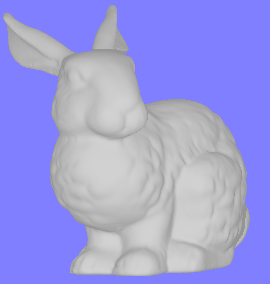
\includegraphics[width=0.3\textwidth]{./Capitulo5/renderBunnyCPU}
    }
    \subfigure[]{
        \label{fig:CvsCudaRenderBunny:b} %% label for second subfigure
        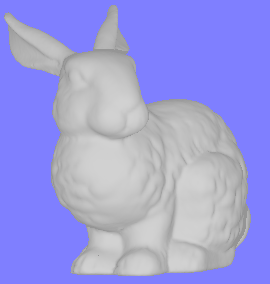
\includegraphics[width=0.3\textwidth]{./Capitulo5/renderBunnyGPU}
    }
    \caption{Render de BUNNY en CPU y en GPU respectivamente.}
    \label{fig:CvsCudaRenderBunny} %% label for entire figure
\end{figure}

Los resultados obtenidos con los casos de prueba DIST\_I, DIST\_II, DIST\_III y BUNNY demuestran que el algoritmo para GPU genera im�genes en un tiempo menor que el algoritmo para CPU. En la Tabla \ref{table:CvsCudaAceleracion} se muestra la aceleraci�n lograda por el algoritmo para GPU para cada caso de prueba. En promedio, considerando los cuatro casos de prueba, el algoritmo para GPU es m�s de once veces m�s r�pido que el algoritmo para CPU. En la Figura \ref{fig:CvsCudaRenderBunny:a} se muestra la imagen generada por el algoritmo implementado en C, mientras que en la Figura \ref{fig:CvsCudaRenderBunny:b} se muestra la imagen generada por el algoritmo implementado en CUDA. Observando estas im�genes el ojo humano no percibe diferencia alguna, entonces el algoritmo para GPU logra una muy buena aceleraci�n con respecto al que ejecuta en CPU y sin perdida en la calidad de imagen.

\begin{table}
\begin{center}
\resizebox{10cm}{!}{
    \small {
    \begin{tabular}{|c|c|c|c|c|}
    \hline
    Escena & Tama�o Grilla & CPU (FPS) & GPU (FPS) & Aceleraci�n\\
    \hline
    DIST\_I & 50x50x50 & 1.4 & 17.2 & 12\\
    \hline
    DIST\_II & 50x50x50 & 1.5 & 20.1 & 14\\
    \hline
    DIST\_III & 50x50x50 & 1.6 & 21.1 & 13\\
    \hline
    BUNNY & 80x80x80 & 4.2 & 23.8 & 6\\
    \hline
    \end{tabular}
    }
}
\caption{Aceleraci�n lograda por algoritmo para GPU.}
\label{table:CvsCudaAceleracion}
\end{center}
\end{table}

\subsection{Comparaci�n entre versiones}

La comparaci�n de rendimiento entre las diferentes versiones del algoritmo para GPU se hizo usando los casos de prueba PRI\_I a PRI\_V. Esta comparaci�n entre versiones consta de dos partes, en la primera se determina la grilla optima para cada caso de prueba y en la segunda se ejecuta cada caso de prueba en cada una de las versiones del algoritmo utilizando su grilla optima.

Para determinar la grilla optima para cada caso de prueba se usa la Versi�n 3 del algoritmo para GPU, ejecutando en el Equipo 3. En la Tabla \ref{table:CompVersionesBuscarGrilla} se muestran los resultados obtenidos al ejecutar los casos de prueba sobre GPU. Observando los resultados se puede concluir que la grilla optima para todos los casos de prueba se construye partiendo en dos cada eje.

Los resultados obtenidos en estas primeras pruebas muestran que a medida que aumenta la cantidad de primitivas con que esta construida la escena aumenta el tiempo de generaci�n de imagen, y por lo tanto disminuyen los FPS. Esto se pensaba antes de ejecutar estos casos de prueba y fue corroborado por los mismos. Tambi�n se pensaba que al aumentar la cantidad de primitivas de la escena aumentar�a la cantidad de voxels que deb�a tener la grilla optima, pero esto no fue validado por los resultados obtenidos. Esto puede deberse a que el incremento de la cantidad de primitivas no es suficientemente grande como para obligar a aumentar la resoluci�n de la grilla.

\begin{table}
\begin{center}
\resizebox{12cm}{!}{
    \begin{tabular}{|c|c|c|c|c|c|c|}
    \hline
    \multirow{2}{*}{\textbf{Escena}}&\multicolumn{6}{|c|}{\textbf{Tama�o de grilla}}\\
    \cline{2-7}
    & 1x1x1 & 2x2x2 & 4x4x4 & 6x6x6 & 10x10x10 & 15x15x15\\
    \hline
    PRI\_I & 18.7 & 36.7 & 32.7 & 29.7 & 27.3 & 24.7\\
    \hline
    PRI\_II & 13.9 & 27.6 & 25.4 & 23.3 & 21.5 & 20.1\\
    \hline
    PRI\_III & 11.3 & 24.5 & 22.8 & 20.9 & 19.2 & 18.0\\
    \hline
    PRI\_IV & 8.4 & 18.5 & 18.0 & 16.5 & 15.9 & 15.1\\
    \hline
    PRI\_V & 6.7 & 16.6 & 15.5 & 14.6 & 13.8 & 13.5\\
    \hline
    \end{tabular}
}
\caption{FPS de PRI\_I,\ldots, PRI\_V en el Equipo 3 sobre GPU.}
\label{table:CompVersionesBuscarGrilla}
\end{center}
\end{table}

Una vez determinada la grilla optima para cada caso de prueba, se ejecuta cada caso utilizando su grilla optima en cada una de las versiones del algoritmo para GPU, en la Tabla \ref{table:CompVersionesFPS} se muestran los resultados obtenidos.

\begin{table}
\begin{center}
\resizebox{12cm}{!}{
    \begin{tabular}{|c|c|c|c|c|}
    \hline
    Escena & Tama�o Grilla Optimo & GPU v1 (FPS) & GPU v2 (FPS) & GPU v3 (FPS)\\
    \hline
    PRI\_I & 2x2x2 & 5.8 & 26.2 & 36.7\\
    \hline
    PRI\_II & 2x2x2 & 5.1 & 20.2 & 27.6\\
    \hline
    PRI\_III & 2x2x2 & 4.9 & 18.2 & 24.5\\
    \hline
    PRI\_IV & 2x2x2 & 4.3 & 14.1 & 18.5\\
    \hline
    PRI\_V & 2x2x2 & 3.9 & 12.6 & 16.6\\
    \hline
    \end{tabular}
}
\caption{FPS de PRI\_I,\ldots, PRI\_V en el Equipo 3 sobre GPU para cada versi�n del algoritmo.}
\label{table:CompVersionesFPS}
\end{center}
\end{table}



\subsection{Comparaci�n entre equipos}

\subsection{Casos m�s exitosos}

\chapter{Conclusiones y trabajo a futuro} % 5 p�ginas mas o menos...

Tomando en cuenta los objetivos definidos al inicio de este trabajo, es posible afirmar que las metas propuestas se lograron exitosamente.

El trabajo se inici� con un estudio general de los distintos m�todos de generaci�n de im�genes por computadora, con mayor profundidad en el algoritmo de \emph{ray tracing} propuesto por Turner Whitted. Posteriormente se continu� con un estudio sobre la utilizaci�n de GPUs como plataforma de ejecuci�n de aplicaciones paralelas. Se investigaron aspectos de la arquitectura de las GPUs, y especialmente herramientas para su programaci�n, y en particular el lenguaje de programaci�n CUDA. Luego se continu� con un relevamiento de los diversos m�todos de aceleraci�n para el algoritmo de \emph{ray tracing}, haciendo �nfasis en los m�todos de aceleraci�n espacial y sus implementaciones sobre GPUs. Por �ltimo, se realiz� un relevamiento del estado del arte de algoritmos de \emph{ray tracing} interactivos, haciendo hincapi� en los algoritmos interactivos implementados sobre arquitecturas multiprocesador de memoria compartida. En estas etapas se adquirieron valiosos conocimientos que luego permitieron realizar el dise�o e implementaci�n de las soluciones propuestas.

Siguiendo un proceso de desarrollo iterativo e incremental, se realiz� la implementaci�n del algoritmo de \emph{ray tracing} sobre GPU paralelizando a nivel de rayos primarios y utilizando una sub-divisi�n espacial uniforme para disminuir la cantidad de evaluaciones de intersecci�n rayo-tri�ngulo. De la primera iteraci�n del proceso surgi� como resultado la versi�n llamada RT-GPU, la cual permite generar im�genes utilizando la GPU para acelerar el c�mputo. Sin embargo, no explota al m�ximo la jerarqu�a de memoria de la GPU y no utiliza un algoritmo de intersecci�n rayo-tri�ngulo optimizado. En la siguiente i\-te\-ra\-ci�n se implement� una estrategia que permite el uso eficiente de la jerarqu�a de memoria de la GPU por parte del algoritmo de \emph{ray tracing}, dando lugar a la versi�n llamada RT-GPU-JM. Posteriormente, en la �ltima iteraci�n se optimiz� el algoritmo de intersecci�n rayo-tri�ngulo y se obtuvo la versi�n final del algoritmo de \emph{ray tracing} implementado sobre GPU, RT-GPU-JM-IR. Asimismo para cada versi�n del algoritmo implementado sobre GPU se implement� una versi�n equivalente para CPU, de forma de evaluar la aceleraci�n lograda al paralelizar el algoritmo sobre GPU.

Otro resultado importante del proyecto es un conjunto de casos de prueba para evaluar algoritmos de iluminaci�n. En una primera etapa se relev� la existencia de \emph{benchmarks} para evaluar este tipo de algoritmo, este relevamiento no permiti� establecer un conjunto de casos de prueba que se adaptaran a la realidad de este proyecto. Por esta raz�n, durante el proceso de implementaci�n se dise�aron y construyeron diversos casos de prueba con el prop�sito de evaluar el desempe�o de cada versi�n del algoritmo. Los casos de prueba fueron dise�ados para cubrir distintos aspectos que se consideraron importantes, por ejemplo puntos d�biles de la estructura de aceleraci�n espacial empleada, desempe�o del algoritmo frente a variaciones de la cantidad de tri�ngulos de la escena, comparaci�n de desempe�o con el estado del arte en la materia y la escalabilidad en las plataformas de prueba.

Los resultados de las pruebas de comparaci�n entre las diferentes versiones del algoritmo para GPU permitieron concluir que el correcto uso de la jerarqu�a de memoria de la GPU es muy importante, ya que la aceleraci�n lograda al pasar de la versi�n RT-GPU a la versi�n RT-GPU-JM fue de m�s de 3x. Se observa tambi�n que la importancia de minimizar los accesos a la memoria global de la GPU, utilizando la memoria compartida disponible entre bloques de threads o la memoria de textura siempre que sea posible, ya que la diferencia de velocidades entre ambas memorias y la memoria global es muy importante. Los resultados obtenidos al realizar pruebas de desempe�o comparando las �ltimas dos versiones implementadas para GPU permiten concluir que es determinante que el \emph{ray tracing} incluya un algoritmo eficiente de chequeo de intersecci�n rayo-tri�ngulo, ya que reduciendo un cuarto la cantidad de operaciones aritm�ticas del chequeo se logr� un 30 \% m�s de velocidad en la generaci�n de la imagen.

Las pruebas de comparaci�n de desempe�o entre la versi�n final del algoritmo para GPU y su correspondiente para CPU permitieron concluir que el objetivo de acelerar el algoritmo de \emph{ray tracing} fue alcanzado con �xito. Todas las pruebas realizadas en este sentido arrojaron que el algoritmo para GPU es m�s r�pido que su correspondiente para CPU, llegando en el mejor caso hasta una aceleraci�n que supera los 13x.

Por otro lado, la comparaci�n entre GPU y CPU permiti� concluir que el tama�o de la grilla de aceleraci�n espacial es independiente del \emph{hardware} donde ejecute el algoritmo y que solo depende de la cantidad de tri�ngulos que componen la escena, ya que para todas las escenas de prueba el tama�o de grilla donde se logran m�s FPS (grilla �ptima) es el mismo en GPU que en CPU.

Se utilizaron cuatro GPUs sobre los sistemas operativos \emph{Windows} y \emph{Linux} para ejecutar los casos de prueba dise�ados, los datos obtenidos permitieron arribar a conclusiones importantes. Los datos de desempe�o obtenidos al ejecutar los mismos casos de prueba sobre distintas plataformas usando la versi�n final del algoritmo para GPU permiten concluir que, para escenas complejas (100.000 tri�ngulos en el contexto de este proyecto), cuanto m�s procesadores posea la GPU m�s r�pido ser� la generaci�n de im�genes mediante el algoritmo de \emph{ray tracing} para CUDA. Asimismo se concluye que para escenas simples el \emph{overhead} introducido por demasiado paralelismo puede afectar el tiempo de generaci�n de imagen. Sin duda la propiedad del algoritmo m�s sobresaliente es la escalabilidad autom�tica en el n�mero de procesadores de la GPU. Este es un beneficio del modelo de programaci�n de CUDA y permite lograr mejores resultados d�a a d�a dado el vertiginoso crecimiento del poder de computo de las GPUs actuales. 

Los resultados de las pruebas de comparaci�n entre la versi�n final del algoritmo implementado en este proyecto y algoritmos desarrollados en otros proyectos similares demostraron que la propuesta del proyecto es competitivo con el estado del arte en la materia, tanto en tiempo de generaci�n como en calidad de imagen. 

Algunos aspectos del trabajo fueron validados mediante la presentaci�n de un art�culo de divulgaci�n cient�fica, \emph{Improving the Performance of the Ray Tracing Algorithm with a GPU}, en las JCC 2010 (Jornadas Chilenas de Computaci�n de 2010). El art�culo fue aceptado por la revisi�n, y ser� incluido en las actas de la conferencia. La versi�n preliminar del art�culo se encuentra en el Ap�ndice \ref{sec:ApendiceArticuloIEEE}.

Como conclusi�n final se puede destacar que el m�todo de aceleraci�n mediante GPU alcanz� tiempos de generaci�n de im�genes que permiten abordar estrategias interactivas para escenas simples. Adem�s la aceleraci�n lograda no implica p�rdida de calidad de imagen, ya que en ninguna de las ejecuciones de los casos de prueba se verificaron diferencias entre im�genes generadas en GPU y en CPU.

A partir del trabajo realizado y las conclusiones extra�das, es posible identificar diversas l�neas de trabajo futuro que se presentan a continuaci�n.

Una primera l�nea de trabajo a futuro es mejorar la estructura de a\-ce\-le\-ra\-ci�n espacial del algoritmo de \emph{ray tracing} implementado. La primer opci�n es optimizar la grilla uniforme que se utiliza actualmente, para optimizarla se puede agregar una etapa m�s a su algoritmo de construcci�n para convertir en una sola caja varias cajas vac�as (o que contengan menos de $k$ tri�ngulos en su interior). Otra opci�n es cambiar la estructura uniforme por una estructura que se adapte m�s a la escena, como la kd-tree. Luego de analizado el estado del arte en esta materia en el transcurso de este proyecto de grado, se piensa que con la estructura kd-tree se obtendr�an mejores resultados. De esta manera se podr�a elevar el l�mite de cantidad de tri�ngulos que tiene el algoritmo actual para renderizar escenas en tiempos interactivos.

En cuanto a mejorar la calidad de las im�genes una l�nea de trabajo es introducir alg�n m�todo de \emph{antialiasing}, como por ejemplo \emph{supersampling}, \emph{adaptive sampling} o \emph{stochastic sampling}. Otra opci�n de mejora en este sentido es eliminar la restricci�n que tiene el algoritmo actual en cuanto a que las escenas no pueden tener objetos reflexivos y transparentes a la vez. Para remover esta restricci�n es necesario implementar un \emph{stack} a nivel de la GPU para manejar un �rbol de rayos en lugar de una lista como se maneja actualmente.

En cuanto a dise�o global del algoritmo una l�nea de trabajo es re-dise�ar los \emph{kernels} utilizados por el algoritmo propuesto. Actualmente existe un \emph{kernel} principal que se encarga de lanzar los rayos primarios, luego lanzar los de sombra, posteriormente lanzar los rayos de reflexi�n y refracci�n y por �ltimo calcular el color del p�xel. Este dise�o tiene problemas porque para escenas complejas el \emph{kernel} principal tiene un tiempo de ejecuci�n demasiado alto y es abortado por el sistema operativo. La estrategia que podr�a solucionar este problema es dividir el \emph{kernel} principal en varios \emph{kernels} m�s peque�os, donde cada uno tenga la responsabilidad de hacer parte del trabajo que hace el principal en la actual implementaci�n.

La siguiente l�nea de trabajo es a m�s largo plazo y consiste en estudiar en profundidad otros algoritmos de generaci�n de im�genes, como \emph{radiosidad} o \emph{photon mapping}, y sus implementaciones sobre GPUs, de modo de aprovechar la experiencia en programaci�n sobre GPUs adquirida en este proyecto de grado aplicada a otras herramientas del �rea.

El impulso de OpenCL como est�ndar de programaci�n de GPUs, para todas las tecnolog�as y no solo para NVIDIA, sugiere otra l�nea de trabajo futuro a m�s largo plazo, que consiste en evaluar la utilizaci�n de otros lenguajes de programaci�n, en particular OpenCL. Tambi�n ser�a interesante lograr un \emph{ray tracing} que utilice varias GPUs y que sea capaz de dividir la generaci�n de la imagen entre ellas.



\appendix

\chapter{Estructuras de datos}\label{sec:ApendiceEstructurasDatos}

En las pr�ximas dos secciones se presentan las estructuras de datos usadas en ambas implementaciones del algoritmo de raytracing de Whitted. Primero se muestra la estructura usada en la implementaci�n para CPU, y luego se muestra la usada en la versi�n implementada para CUDA.

Es importante conocer que en las primeras etapas del proyecto las dos versiones usaban la misma estructura de datos. A medida que el proyecto fue avanzando la estructura para CUDA fue evolucionando hasta llegar a la actual. Por no contar con experiencia en programaci�n sobre CUDA la estructura tuvo que ir evolucionando junto con el aprendizaje de la herramienta.

\section{Algoritmo para CPU}

\begin{algorithm}[H]
    \caption{Estructura de datos para almacenar la escena. Parte I.}
    \label{alg:EstructuraEscenaCI}
    \begin{algorithmic}
        \State typedef struct $\{$
            \State $\ \ \ \ $ObjetoEscena* objetos;
	        \State $\ \ \ \ $int cant\_objetos;
            \State $\ \ \ \ $Camara camara;
            \State $\ \ \ \ $Triangulo plano\_de\_vista;
            \State $\ \ \ \ $Luz* luces;
            \State $\ \ \ \ $int cant\_luces;
            \State $\ \ \ \ $UniformGrid grilla;
            \State $\ \ \ \ $Material* materiales;
            \State $\ \ \ \ $int cant\_materiales;
        \State $\}$ Escena;
        \\
        \State typedef struct $\{$
            \State $\ \ \ \ $float3 v1;
            \State $\ \ \ \ $float3 v2;
            \State $\ \ \ \ $float3 v3;
        \State $\}$ Triangulo;
        \\
        \State typedef struct $\{$
            \State $\ \ \ \ $TipoObjeto tipo;
            \State $\ \ \ \ $Triangulo tri;
            \State $\ \ \ \ $Triangulo normales;
            \State $\ \ \ \ $int id\_material;
        \State $\}$ ObjetoEscena;
        \\
        \State typedef enum $\{$
            \State $\ \ \ \ $Triangle,
        	\State $\ \ \ \ $Sphere\\
        $\}$ TipoObjeto;
    \end{algorithmic}
\end{algorithm}

\begin{algorithm}[H]
    \caption{Estructura de datos para almacenar la escena. Parte II.}
    \label{alg:EstructuraEscenaCII}
    \begin{algorithmic}
        \State typedef struct $\{$
            \State $\ \ \ \ $float3 ojo;
            \State $\ \ \ \ $float3 direccion;
            \State $\ \ \ \ $float3 up;
        \State $\}$ Camara;
        \\
        \State typedef struct $\{$
            \State $\ \ \ \ $float3 posicion;
            \State $\ \ \ \ $float3 color;
        \State $\}$ Luz;
        \\
        \State typedef struct $\{$
            \State $\ \ \ \ $float3 dimension;
            \State $\ \ \ \ $BoundingBox bbEscena;
            \State $\ \ \ \ $int* voxels;
            \State $\ \ \ \ $int* listasGrid;
        \State $\}$ UniformGrid;
        \\
        \State typedef struct $\{$
            \State $\ \ \ \ $float3 diffuse\_color;
            \State $\ \ \ \ $float3 ambient\_color;
            \State $\ \ \ \ $float3 specular\_color;
            \State $\ \ \ \ $float refraction;
            \State $\ \ \ \ $float reflection;
            \State $\ \ \ \ $float transparency;
            \State $\ \ \ \ $int coef\_at\_especular;
        \State $\}$ Material;
        \\
        \State typedef struct $\{$
            \State $\ \ \ \ $float3 minimum;
            \State $\ \ \ \ $float3 maximum;
        \State $\}$ BoundingBox;
    \end{algorithmic}
\end{algorithm}

\section{Algoritmo para GPU}

\begin{algorithm}[H]
    \caption{Estructura de datos para almacenar la escena. Parte I.}
    \label{alg:EstructuraEscenaCUDAI}
    \begin{algorithmic}
        \State typedef struct $\{$
            \State $\ \ \ \ $Triangulo* triangulos;
            \State $\ \ \ \ $Triangulo* normales;
	        \State $\ \ \ \ $int cant\_objetos;
            \State $\ \ \ \ $Camara camara;
            \State $\ \ \ \ $Triangulo plano\_de\_vista;
            \State $\ \ \ \ $Luz* luces;
            \State $\ \ \ \ $int cant\_luces;
            \State $\ \ \ \ $UniformGrid grilla;
            \State $\ \ \ \ $Material* materiales;
            \State $\ \ \ \ $int cant\_materiales;
        \State $\}$ Escena;
        \\
        \State typedef struct $\{$
            \State $\ \ \ \ $float4 v1;
            \State $\ \ \ \ $float4 v2;
            \State $\ \ \ \ $float4 v3;
        \State $\}$ Triangulo;
    \end{algorithmic}
\end{algorithm}

\begin{algorithm}[H]
    \caption{Estructura de datos para almacenar la escena. Parte II.}
    \label{alg:EstructuraEscenaCUDAII}
    \begin{algorithmic}
        \State typedef struct $\{$
            \State $\ \ \ \ $float3 ojo;
            \State $\ \ \ \ $float3 direccion;
            \State $\ \ \ \ $float3 up;
        \State $\}$ Camara;
        \\
        \State typedef struct $\{$
            \State $\ \ \ \ $float4 posicion;
            \State $\ \ \ \ $float4 color;
        \State $\}$ Luz;
        \\
        \State typedef struct $\{$
            \State $\ \ \ \ $float3 dimension;
            \State $\ \ \ \ $BoundingBox bbEscena;
            \State $\ \ \ \ $int* voxels;
            \State $\ \ \ \ $int* listasGrid;
        \State $\}$ UniformGrid;
        \\
        \State typedef struct $\{$
            \State $\ \ \ \ $float4 diffuse\_color;
            \State $\ \ \ \ $float4 ambient\_color;
            \State $\ \ \ \ $float4 specular\_color;
            \State $\ \ \ \ $float4 others;
        \State $\}$ Material;
        \\
        \State typedef struct $\{$
            \State $\ \ \ \ $float3 minimum;
            \State $\ \ \ \ $float3 maximum;
        \State $\}$ BoundingBox;
    \end{algorithmic}
\end{algorithm} 

\newpage
\bibliography{./../bibliografia}
\bibliographystyle{plain}

\end{document} 